% Preámbulo de la colección de problemas.
% Edítalo a tu gusto; debe terminar justo después de \begin{document}
% (y, si quieres, \maketitle / \tableofcontents). El generador añade el cuerpo
% con los \input de cada problema y cierra con \end{document}.
\documentclass[11pt]{article}
\usepackage[utf8]{inputenc}
\usepackage[T1]{fontenc}
\usepackage[spanish,es-noshorthands]{babel}
\usepackage{amsmath}
\usepackage{amssymb}
\usepackage{graphicx}
\usepackage{comment}
\usepackage{booktabs}
\usepackage{multirow}
\usepackage{enumitem}
\usepackage{float}
\usepackage{tikz}
\usetikzlibrary{arrows, arrows.meta, positioning, calc, automata, graphs, shapes.geometric}
\usepackage{pgfplots}
\pgfplotsset{compat=1.18}
% --- Estilos TikZ personalizados (problemas de grafos) -----------------
% Ajusta estas definiciones a las de tu preámbulo original si difieren.
\tikzstyle{arn_n}=[fill=black, text=white, draw=black, circle, minimum size=22pt, inner sep=0pt]
\tikzstyle{arn_r}=[fill=red,   text=white, draw=black, circle, minimum size=22pt, inner sep=0pt]
\tikzstyle{arn_x}=[fill=white, text=black, draw=black, circle, minimum size=22pt, inner sep=0pt]
% -----------------------------------------------------------------------
\usepackage[margin=2.5cm]{geometry}

\title{Colección de problemas de Programación Lineal}
\author{}
\date{}

\begin{document}
\maketitle
\tableofcontents
\clearpage

\section{01a dos fases a}
\input{ejercicios/01a_dos_fases_a}
\subsection*{Solución}
Formulación del problema de la primera fase:

\begin{equation}
\begin{split}
\mbox{max. } z' = -1a_1\\
s.a.:\\
4x_1+2x_2+1a_1 = 80\\
2x_1+3x_2+1h_2 = 60\\
x_1,\,x_2,\,h_2,\,a_1\geq 0\end{split}
\end{equation}

Resolución del problema:

\begin{center}
\begin{tabular}{c|c|cccc|}
 & $z$ & $x_1$ & $x_2$ & $h_2$ & $a_1$\\ 
Fase 1 & 80 & 4 & 2 & 0 & 0 \\ 
Fase 2 & 0 & 1 & 4 & 0 & 0 \\ 
\hline
$a_1$ & 80  & 4 & 2 & 0 & 1\\ 
$h_2$ & 60  & 2 & 3 & 1 & 0\\ 
\hline
Fase 1 & 0 & 0 & 0 & 0 & -1 \\ 
Fase 2 & -20 & 0 & 7/2 & 0 & -1/4 \\ 
\hline
$x_1$ & 20  & 1 & 1/2 & 0 & 1/4\\ 
$h_2$ & 20  & 0 & 2 & 1 & -1/2\\ 
\hline
Fase 2 & -55 & 0 & 0 & -7/4 & 5/8 \\ 
\hline
$x_1$ & 15  & 1 & 0 & -1/4 & 3/8\\ 
$x_2$ & 10  & 0 & 1 & 1/2 & -1/4\\ 
\hline
\end{tabular}
\end{center}


\clearpage
\section{01b dos fases b}
Dado el siguiente problema, $P$, de programación lineal:

\begin{equation}
\begin{split}
\mbox{max. } z = 4x_1 + 2x_2\\
s.a.:\\
4x_1 + 1x_2  = 60\\
2x_1 + 4x_2  \leq 80\\
x_1,\,\,x_2\geq 0\\
\end{split}
\end{equation}

\begin{itemize}
    \item \textbf{Formular} el problema correspondiente a la primera fase (correspondiente a la aplicación del método de las dos fases).
    \item \textbf{Resolver} el problema $P$ mediante el método de la matriz completa aplicando el método de las dos fases.
\end{itemize}
\subsection*{Solución}
Formulación del problema de la primera fase:

\begin{equation}
\begin{split}
\mbox{max. } z' = -1a_1\\
s.a.:\\
4x_1+1x_2+1a_1 = 60\\
2x_1+4x_2+1h_2 = 80\\
x_1,\,x_2,\,h_2,\,a_1\geq 0\end{split}
\end{equation}

Resolución del problema:

\begin{center}
\begin{tabular}{c|c|cccc|}
    & $z$ & $x_1$ & $x_2$ & $h_2$ & $a_1$\\ 
Fase 1 & 60 & 4 & 1 & 0 & 0 \\ 
Fase 2 & 0 & 4 & 2 & 0 & 0 \\ 
\hline
$a_1$ & 60  & 4 & 1 & 0 & 1\\ 
$h_2$ & 80  & 2 & 4 & 1 & 0\\ 
\hline
Fase 1 & 0 & 0 & 0 & 0 & -1 \\ 
Fase 2 & -60 & 0 & 1 & 0 & -1 \\ 
\hline
$x_1$ & 15  & 1 & 1/4 & 0 & 1/4\\ 
$h_2$ & 50  & 0 & 7/2 & 1 & -1/2\\ 
\hline
Fase 2 & -520/7 & 0 & 0 & -2/7 & -6/7 \\ 
\hline
$x_1$ & 80/7  & 1 & 0 & -1/14 & 2/7\\ 
$x_2$ & 100/7  & 0 & 1 & 2/7 & -1/7\\ 
\hline
\end{tabular}
\end{center}





\clearpage
\section{02a inversa base a}
Dado el siguiente problema de programación lineal:

\begin{equation}
\begin{split}
\mbox{max. } z = 3x_1 + 2x_2\\
s.a.:\\
2x_1 + 4x_2  \leq 80\\
4x_1 + 3x_2  = 60\\
1x_1 + 1x_2  \geq 10\\
x_1,\,\,x_2\geq 0\\
\end{split}
\end{equation}

Su solución óptima es la correspondiente a la siguiente tabla:

\begin{center}
\begin{tabular}{c|c|cccc|}
 & $z$ & $x_1$ & $x_2$ & $h_1$ & $h_3$\\ 
       & -45 & 0 & -1/4 & 0 & 0  \\ 
\hline
$h_1$ & 50  & 0 & 5/2 & 1 & 0 \\ 
$h_3$ & 5  & 0 & -1/4 & 0 & 1 \\ 
$x_1$ & 15  & 1 & 3/4 & 0 & 0 \\ 
\hline
\end{tabular}
\end{center}


Se pide calcular la base y la inversa de la base de la solución óptima.
\subsection*{Solución}
\begin{center}
\begin{tabular}{c|c|cccc|}
& $z$ & $x_1$ & $x_2$ & $h_1$ & $h_3$\\ 
    & -45 & 0 & -1/4 & 0 & 0  \\ 
\hline
$h_1$ & 50  & 0 & 5/2 & 1 & 0 \\ 
$h_3$ & 5  & 0 & -1/4 & 0 & 1 \\ 
$x_1$ & 15  & 1 & 3/4 & 0 & 0 \\ 
\hline
\end{tabular}
\end{center}


Base de la solución óptima:

\begin{equation}
B = \begin{pmatrix}
1 & 0 & 2\\
0 & 0 & 4\\
0 & -1 & 1\\
\end{pmatrix}
\end{equation}

Inversa de la base:

\begin{equation}
B^{-1} = 
\begin{pmatrix}
1 & \frac{-1}{2} & 0\\
0 & \frac{1}{4} & -1\\
0 & \frac{1}{4} & 0\\
\end{pmatrix}
\end{equation}
\clearpage
\section{02b inversa base b}
Dado el siguiente problema de programación lineal:

\begin{equation}
\begin{split}
\mbox{max. } z = 4x_1 + 2x_2\\
s.a.:\\
4x_1 + 4x_2  \leq 100\\
2x_1 + 3x_2  = 50\\
1x_1 + 2x_2  \geq 10\\
x_1,\,\,x_2\geq 0\\
\end{split}
\end{equation}

Su solución óptima es la correspondiente a la siguiente tabla:

\begin{center}
\begin{tabular}{c|c|cccc|}
 & $z$ & $x_1$ & $x_2$ & $h_1$ & $h_3$\\ 
 & -100 & 0 & 0 & -2 & 0  \\ 
\hline
$x_1$ & 25  & 1 & 0 & 3/4 & 0 \\ 
$h_3$ & 15  & 0 & 0 & -1/4 & 1 \\ 
$x_2$ & 0  & 0 & 1 & -1/2 & 0 \\ 
\hline
\end{tabular}
\end{center}

% \begin{center}
% \begin{tabular}{c|c|cccccc|}
%  & $z$ & $x_1$ & $x_2$ & $h_1$ & $h_3$ & $a_2$ & $a_3$\\ 
%  & -100 & 0 & 0 & -2 & 0 & 2 & 0 \\ 
% \hline
% $x_1$ & 25  & 1 & 0 & 3/4 & 0 & -1 & 0\\ 
% $h_3$ & 15  & 0 & 0 & -1/4 & 1 & 1 & -1\\ 
% $x_2$ & 0  & 0 & 1 & -1/2 & 0 & 1 & 0\\ 
% \hline
% \end{tabular}
% \end{center}



Se pide calcular la base y la inversa de la base de la solución óptima.
\subsection*{Solución}
\begin{center}
\begin{tabular}{c|c|cccccc|}
 & $z$ & $x_1$ & $x_2$ & $h_1$ & $h_3$ & $a_2$ & $a_3$\\ 
 & -100 & 0 & 0 & -2 & 0 & 2 & 0 \\ 
\hline
$x_1$ & 25  & 1 & 0 & 3/4 & 0 & -1 & 0\\ 
$h_3$ & 15  & 0 & 0 & -1/4 & 1 & 1 & -1\\ 
$x_2$ & 0  & 0 & 1 & -1/2 & 0 & 1 & 0\\ 
\hline
\end{tabular}
\end{center}

% \begin{center}
% \begin{tabular}{c|c|cccccc|}
%  & $z$ & $x_1$ & $x_2$ & $h_1$ & $h_3$ & $a_2$ & $a_3$\\ 
% Phase 2 & -100 & 0 & 0 & -2 & 0 & 2 & 0 \\ 
% \hline
% $x_1$ & 25  & 1 & 0 & 3/4 & 0 & -1 & 0\\ 
% $h_3$ & 15  & 0 & 0 & -1/4 & 1 & 1 & -1\\ 
% $x_2$ & 0  & 0 & 1 & -1/2 & 0 & 1 & 0\\ 
% \hline
% \end{tabular}
% \end{center}


Base de la solución óptima:

\begin{equation}
B = \begin{pmatrix}
4 & 0 & 4\\
2 & 0 & 3\\
1 & -1 & 2\\
\end{pmatrix}
\end{equation}


Inversa de la base:

\begin{equation}
B^{-1} = 
\begin{pmatrix}
\frac{3}{4} & -1 & 0\\
\frac{-1}{4} & 1 & -1\\
\frac{-1}{2} & 1 & 0\\
\end{pmatrix}
\end{equation}
\clearpage
\section{03a empresa minera a}
\input{ejercicios/03a_empresa_minera_a}
\subsection*{Solución}
\begin{enumerate}
\item Los valores de las variables y su interpretación son los siguientes:

\begin{center}
\begin{tabular}{c|c|cccccccc|}
 & $z$ & $x_1$ & $x_2$ & $x_3$ & $x_4$ & $h_1$ & $h_3$ & $a_2$ & $a_3$\\ 
\hline
Phase 1 & 4 & $-1/5$ & 0 & $2/5$ & 0 & 0 & -1 & $-6/5$ & 0 \\ 
Phase 2 & -10000 & -250 & 0 & -100 & 0 & -100 & 0 & 0 & 0 \\ 
\hline
$x_4$ & 52  & $22/5$ & 0 & $16/5$ & 1 & 1 & 0 & $-3/5$ & 0\\ 
$x_2$ & 16  & $1/5$ & 1 & $3/5$ & 0 & 0 & 0 & $1/5$ & 0\\ 
$a_3$ & 4  & $-1/5$ & 0 & $2/5$ & 0 & 0 & -1 & $-1/5$ & 1\\ 
\hline
Phase 1 & 0 & 0 & 0 & 0 & 0 & 0 & 0 & -1 & -1 \\ 
Phase 2 & -9000 & -300 & 0 & 0 & 0 & -100 & -250 & -50 & 250 \\ 
\hline
$x_4$ & 20  & 6 & 0 & 0 & 1 & 1 & 8 & 1 & -8\\ 
$x_2$ & 10  & $1/2$ & 1 & 0 & 0 & 0 & $3/2$ & $1/2$ & $-3/2$\\ 
$x_3$ & 10  & $-1/2$ & 0 & 1 & 0 & 0 & $-5/2$ & $-1/2$ & $5/2$\\ 
\hline
\end{tabular}
\end{center}


\begin{itemize}
    \item $x_1 = 0$: no se produce aleación blanda. 
    \item $x_2 = 10$: se producen 10 toneladas de aleación dura.
    \item $x_3 = 10$: se producen 10 toneladas de aleación fuerte.
    \item $x_4 = 20$: se venden 20 toneladas de mineral rojo.
    \item $h_1 = 0$: todo el mineral rojo se emplea en aleaciones o bien se vende.
    \item $h_3 = 0$: se cumple el compromiso comercial por la cantidad mínima establecida (20 toneladas).
\end{itemize}

\item El precio sombra de la restricción 2 es $\pi^B_2 = 50$, con lo que por cada tonelada de mineral negro que la empresa pudiera extraer adicionalmente a las 80 que ya extrae el beneficio aumentaría en 50 euros, por lo que la empresa sí estaría interesada en extraer más que esas 80 toneladas, siempre y cuando el coste de extracción no superase un coste de 50 euros/tonelada.

\item Las columnas de las variables $h_1$ y $x_4$ en la matriz $A$ con idénticas: $A_{x_4} = A_{h_1} = (1\; 0\; 0)^T$ y sus respectivos criterios del simplex son:


$V^B_{x_4} = c_{x_4} - c^BB^{-1}A_{x_4} = 100 - c^BB^{-1}(1\; 0\; 0)^T$

$V^B_{h_1} = c_{h_1} - c^BB^{-1}A_{x_4} = 0 - c^BB^{-1}(1\; 0\; 0)^T$

Con lo que siempre se cumplirá $V^B_{x_4} > V^B_{h_1}$ y dado que las dos actividades son linealmente dependientes las dos no pueden ser simultáneamente básicas, así que la variable que será básica en la solución óptima será necesariamente $x_4$ y la variable $h_1$ será no básica y, por lo tanto, cero.

El términos de la situación de la empresa, lo anterior se pone de manifiesto en el hecho de que nunca le va a interesar dejar de utilizar mineral rojo ($h_1 > 0 $) porque la venta de ese mineral ($x_4 > 0$) permitirá mejorar el beneficio.

\item Para obtener el intervalo, se admite un valor del compromiso comercial genérico, $b_3$

\begin{equation}
\begin{split}
u^B = B^{-1}b = 
\begin{pmatrix}
1 & 1 & -8\\
0 & \frac{1}{2} & \frac{-3}{2}\\
0 & \frac{-1}{2} & \frac{5}{2}\\
\end{pmatrix}
\begin{pmatrix}
100\\
80\\
b_3\\
\end{pmatrix}
\geq 0 \Rightarrow
\begin{pmatrix}
180 - 8b_3\\
\frac{80-3b_3}{2}\\
\frac{-80+5b_3}{2}\\
\end{pmatrix}
\geq 0 \Rightarrow
16 \leq b_3 \leq \frac{45}{2} < \frac{80}{3}
\end{split}
\end{equation}

Mientras el compromiso comercial sea igual o mayor a 16 toneladas y menor o igual a 22.5 toneladas, las variables básicas de la solución son las misma y, por lo tanto, la gama de productos se mantiene.

\item $x_2 \leq 8 \Rightarrow x_2 + h_4 = 8$

\begin{center}
\begin{tabular}{c|c|ccccccccc|}
      & $z$   & $x_1$   & $x_2$   & $x_3$   & $x_4$ & $h_1$ & $h_3$ & $a_2$ & $a_3$ & $h_4$\\ 
      & -9000 & -300    & 0       & 0       & 0     & -100  & -250  & -50   & 250   & 0\\ 
\hline
$x_4$ & 20    & 6       & 0       & 0       & 1     & 1     & 8     & 1     & -8    & 0\\ 
$x_2$ & 10    & 1/2     & 1       & 0       & 0     & 0     & 3/2   & 1/2   & -3/2  & 0\\ 
$x_3$ & 10    & -1/2    & 0       & 1       & 0     & 0     & -5/2  & -1/2  & 5/2   & 0\\
\hline
      &  8    & 0       & 1       & 0       & 0     & 0     & 0     & 0     & 0     & 1\\
\hline
$h_4$ &  -2   & -1/2    & 0      & 0       & 0     & 0     & -3/2  & -1/2  & 3/2   & 1\\
\hline      
\end{tabular}
\end{center}

Podemos aplicar Lemke:

\begin{center}
\begin{tabular}{c|c|ccccccccc|}
      & $z$   & $x_1$   & $x_2$   & $x_3$   & $x_4$ & $h_1$ & $h_3$ & $a_2$ & $a_3$ & $h_4$\\ 
      & -9000 & -300    & 0       & 0       & 0     & -100  & -250  & -50   & 250   & 0\\ 
\hline
$x_4$ & 20    & 6       & 0       & 0       & 1     & 1     & 8     & 1     & -8    & 0\\ 
$x_2$ & 10    & 1/2     & 1       & 0       & 0     & 0     & 3/2   & 1/2   & -3/2  & 0\\ 
$x_3$ & 10    & -1/2    & 0       & 1       & 0     & 0     & -5/2  & -1/2  & 5/2   & 0\\
$h_4$ &  -2   & -1/2    & 0       & 0       & 0     & 0     & -3/2  & -1/2  & 3/2   & 1\\
\hline      
  &-26000/3   & -150    & -500/3  & 0       & 0     & 0     & 0     & 100/3 & 0     &  -500/3\\ 
\hline
$x_4$ &  28/3 &         &         &         &       &       & 0     &       &       & \\ 
$x_2$ &  8    &         &         &         &       &       & 0     &       &       &  \\ 
$x_3$ & 40/3  &         &         &         &       &       & 0     &       &       &  \\
$h_3$ & 4/3   & 1/3     & 0       & 0       & 0     & 0     & 1     & 1/3   & -1    & -2/3\\
\hline      
\end{tabular}
\end{center}

Los valores de las variables y su interpretación son los siguientes:
\begin{itemize}
    \item $x_1 = 0$: no se produce aleación blanda. 
    \item $x_2 = 5$: se producen 5 toneladas de aleación dura.
    \item $x_3 = 40/3$: se producen 40/3 toneladas de aleación fuerte.
    \item $x_4 = 28/3$: se venden 28/3 toneladas de mineral rojo.
    \item $h_1 = 0$: todo el mineral rojo se emplea en aleaciones o bien se vende.
    \item $h_3 = 4/3$: se cumple el compromiso comercial superando en 4/3 de tonelada la cantidad mínima establecida (20 toneladas).
\end{itemize}
    
Ahora el beneficio es menor e igual a 26000/3 euros.

\end{enumerate}
\clearpage
\section{03b empresa minera b}
Una empresa minera extrae \textbf{80 toneladas} de mineral rojo y \textbf{60 toneladas} de mineral negro cada semana. Estos pueden ser tratados de diferentes maneras para producir tres diferentes aleaciones, blanda, dura o fuerte. Para producir 1 tonelada de aleación blanda se requiere \textbf{4 toneladas} de mineral rojo y \textbf{2 toneladas} de negro. Para la aleación dura los requisitos son \textbf{1 toneladas} de rojo y \textbf{4 toneladas} de negro, mientras que para la aleación fuerte son \textbf{2 toneladas} de rojo y \textbf{4 toneladas} de negro. La ganancia por tonelada de la venta de las aleaciones (después de considerar los costos de producción, pero no los de extracción, que se consideran fijos) son \textbf{300}, \textbf{200} y \textbf{300 euros} por tonelada de aleación blanda, dura y fuerte, respectivamente.

Además, el mineral rojo se puede vender a \textbf{50} euros la tonelada y el mineral negro se debe emplear al completo.

Existe un compromiso comercial de servir al menos \textbf{10} toneladas conjuntamente entre las aleaciones dura y fuerte.

\begin{equation}
\begin{split}
\mbox{max. } z = 300x_1 + 200x_2 + 300x_3 + 50x_4\\
s.a.:\\
4x_1 + 1x_2 + 2x_3 + 1x_4 \leq 80\\
2x_1 + 4x_2 + 4x_3 + 0x_4 = 60\\
0x_1 + 1x_2 + 1x_3 + 0x_4 \geq 10\\
x_1,\,\,x_2,\,\,x_3,\,\,x_4\geq 0\\
\end{split}
\end{equation}

Donde $x_1$, $x_2$ y $x_3$ representan las producciones de aleación blanda, dura y fuerte (en toneladas), respectivamente y $x_4$ son las toneladas de mineral rojo de venta en el mercado.

La siguiente tabla es la correspondiente a la solución óptima del problema original

\begin{center}
\begin{tabular}{c|c|cccccccc|}
 & $z$ & $x_1$ & $x_2$ & $x_3$ & $x_4$ & $h_1$ & $h_3$ & $a_2$ & $a_3$\\ 
Phase 2 & -7000 & 0 & -50 & 0 & 0 & -50 & 0 & -50 & 0 \\ 
\hline
$x_4$ & 20  & 0 & -1 & 0 & 1 & 1 & -6 & -2 & 6\\ 
$x_1$ & 10  & 1 & 0 & 0 & 0 & 0 & 2 & 1/2 & -2\\ 
$x_3$ & 10  & 0 & 1 & 1 & 0 & 0 & -1 & 0 & 1\\ 
\hline
\end{tabular}
\end{center}


\begin{enumerate}

\item \textbf{Interpretar} el resultado y explicar el plan de extracción y el significado de los valores de las variables de holgura.


\item Dado que el mineral negro se debe emplear completo, \textbf{justificar} si la empresa estaría interesada en extraer más o menos cantidad que las 60 toneladas semanales.

\item \textbf{Justificar haciendo uso de los fundamentos del método del simplex} por qué, sin necesidad de resolver el problema, se podría afirmar que en la solución óptima $h_1$ nunca puede tomar un valor diferente de 0.

\item Cuál es el intervalo relativo a la cantidad del compromiso comercial (aleaciones dura y fuerte) dentro del cual se mantiene la gama de producción correspondiente a la solución óptima.

\item La empresa está interesada en saber cuál sería el impacto sobre su plan de producción y sobre su beneficio si, una determinada semana, no pudiera vender (y, por lo tanto, no produciría) más de 8 toneladas de aleación fuerte.

% \begin{comment}
% Podemos preguntar sobre el V^B d ela variable artificiales o su signo o su relación con la restricción...
% \end{comment}

\end{enumerate}


% \begin{comment}
% \begin{center}
% \begin{tabular}{c|c|cccccc|}
%  & $z$ & $x_1$ & $x_2$ & $h_1$ & $h_3$ & $a_2$ & $a_3$\\ 
% Phase 1 & 0 & 0 & 0 & 0 & 0 & 0 & -1 \\ 
% Phase 2 & -45 & 0 & -1/4 & 0 & 0 & -3/4 & 0 \\ 
% \hline
% $h_1$ & 50  & 0 & 5/2 & 1 & 0 & -1/2 & 0\\ 
% $h_3$ & 5  & 0 & -1/4 & 0 & 1 & 1/4 & -1\\ 
% $x_1$ & 15  & 1 & 3/4 & 0 & 0 & 1/4 & 0\\ 
% \hline
% \end{tabular}
% \end{center}

% \end{comment}
\subsection*{Solución}
\begin{enumerate}


\item Los valores de las variables y su interpretación son los siguientes:
\begin{itemize}
    \item $x_1 = 10$: se producen 10 toneladas de aleación blanda. 
    \item $x_2 = 0$: no se produce aleación blanda dura.
    \item $x_3 = 10$: se producen 10 toneladas de aleación fuerte.
    \item $x_4 = 20$: se venden 20 toneladas de mineral rojo.
    \item $h_1 = 0$: todo el mineral rojo se emplea en aleaciones o bien se vende.
    \item $h_3 = 0$: se cumple el compromiso comercial por la cantidad mínima establecida 10 toneladas).
\end{itemize}

\item El precio sombra de la restricción 2 es $\pi^B_2 = 50$, con lo que por cada tonelada de mineral negro que la empresa pudiera extraer adicionalmente a las 60 que ya extrae el beneficio aumentaría en 50 euros, por lo que la empresa sí estaría interesada en extraer más que esas 60 toneladas, siempre y cuando el coste de extracción no superase un coste de 50 euros/tonelada.

\item Las columnas de las variables $h_1$ y $x_4$ en la matriz $A$ con idénticas: $A_{x_4} = A_{h_1} = (1\; 0\; 0)^T$ y sus respectivos criterios del simplex son:


$V^B_{x_4} = c_{x_4} - c^BB^{-1}A_{x_4} = 100 - c^BB^{-1}(1\; 0\; 0)^T$

$V^B_{h_1} = c_{h_1} - c^BB^{-1}A_{x_4} = 0 - c^BB^{-1}(1\; 0\; 0)^T$

Con lo que siempre se cumplirá $V^B_{x_4} > V^B_{h_1}$ y dado que las dos actividades son linealmente dependientes las dos no pueden ser simultáneamente básicas, así que la variable que será básica en la solución óptima será necesariamente $x_4$ y la variable $h_1$ será no básica y, por lo tanto, cero.

El términos de la situación de la empresa, lo anterior se pone de manifiesto en el hecho de que nunca le va a interesar dejar de utilizar mineral rojo ($h_1 > 0 $) porque la venta de ese mineral ($x_4 > 0$) permitirá mejorar el beneficio.

\item Para obtener el intervalo, se admite un valor del compromiso comercial genérico, $b_3$

\begin{equation}
\begin{split}
u^B = B^{-1}b = 
\begin{pmatrix}
1 & -2 & 6\\
0 & \frac{1}{2} & -2\\
0 & 0 & 1\\
\end{pmatrix}
\begin{pmatrix}
80\\
60\\
b_3\\
\end{pmatrix}
\geq 0 \Rightarrow
\begin{pmatrix}
80 - 120 + 6b_3\\
30-2b_3\\
b_3\\
\end{pmatrix}
\geq 0 \Rightarrow
0 < \frac{20}{3} \leq b_3 \leq 15 
\end{split}
\end{equation}

Mientras exista compromiso comercial por cualquier cantidad  menor o igual a $\frac{20}{3}$ toneladas, las variables básicas de la solución son las misma y, por lo tanto, la gama de productos se mantiene.

\item $x_3 \leq 8 \Rightarrow x_3 + h_4 = 8$


% \begin{center}
% \begin{tabular}{c|c|cccccccc|}
%  & $z$ & $x_1$ & $x_2$ & $x_3$ & $x_4$ & $h_1$ & $h_3$ & $a_2$ & $a_3$\\ 
%       & -7000 & 0 & -50 & 0 & 0 & -50 & 0 & -50 & 0 \\ 
% \hline
% $x_4$ & 20  & 0 & -1 & 0 & 1 & 1 & -6 & -2 & 6\\ 
% $x_1$ & 10  & 1 & 0 & 0 & 0 & 0 & 2 & 1/2 & -2\\ 
% $x_3$ & 10  & 0 & 1 & 1 & 0 & 0 & -1 & 0 & 1\\ 
% \hline
% \end{tabular}
% \end{center}

\begin{center}
\begin{tabular}{c|c|ccccccccc|}
      & $z$   & $x_1$   & $x_2$   & $x_3$   & $x_4$ & $h_1$ & $h_3$ & $a_2$ & $a_3$ & $h_4$\\ 
      & -7000 & 0       & -50     & 0       & 0     & -50   & 0     & -50   & 0     & 0    \\ 
\hline
$x_4$ & 20    & 0       & -1      & 0       & 1     & 1     & -6    & -2    & 6     & 0    \\ 
$x_1$ & 10    & 1       & 0       & 0       & 0     & 0     & 2     & 1/2   & -2    & 0    \\ 
$x_3$ & 10    & 0       & 1       & 1       & 0     & 0     & -1    & 0     & 1     & 0    \\
\hline
      &  8    & 0       & 0       & 1       & 0     & 0     & 0     & 0     & 0     & 1\\
\hline
$h_4$ &  -2   & 0       & -1      & 0       & 0     & 0     & 1     & 0     & -1    & 1\\
\hline      
\end{tabular}
\end{center}

Podemos aplicar Lemke:

\begin{center}
\begin{tabular}{c|c|ccccccccc|}
      & $z$   & $x_1$   & $x_2$   & $x_3$   & $x_4$ & $h_1$ & $h_3$ & $a_2$ & $a_3$ & $h_4$\\ 
      & -7000 & 0       & -50     & 0       & 0     & -50   & 0     & -50   & 0     & 0    \\ 
\hline
$x_4$ & 20    & 0       & -1      & 0       & 1     & 1     & -6    & -2    & 6     & 0  \\ 
$x_1$ & 10    & 1       & 0       & 0       & 0     & 0     & 2     & 1/2   & -2    & 0  \\ 
$x_3$ & 10    & 0       & 1       & 1       & 0     & 0     & -1    & 0     & 1     & 0  \\
$h_4$ &  -2   & 0       & -1      & 0       & 0     & 0     & 1     & 0     & -1    & 1  \\
\hline      
      & -6900 & 0       & 0       & 0       & 0     &       &       &       &       &     \\ 
\hline
$x_4$ & 22    &         & 0       &         &       &       & 0     &       &       &     \\ 
$x_1$ & 10    &         & 0       &         &       &       & 0     &       &       &     \\ 
$x_3$ & 8     &         & 0       &         &       &       & 0     &       &       &     \\
$x_2$ & 2     & 0       & 1       & 0       & 0     & 0     & -1    & 0     & 1     &  -1 \\
\hline      
\end{tabular}
\end{center}

Los valores de las variables y su interpretación son los siguientes:
\begin{itemize}
    \item $x_1 = 10$: se producen 10 toneladas de aleación blanda. 
    \item $x_2 = 2$: se producen 2 toneladas de aleación dura.
    \item $x_3 = 8$: se producen 8 toneladas de aleación fuerte.
    \item $x_4 = 22$: se venden 22 toneladas de mineral rojo.
    \item $h_1 = 0$: todo el mineral rojo se emplea en aleaciones o bien se vende.
    \item $h_3 = 0$: se cumple el compromiso comercial por la cantidad mínima establecida 10 toneladas).
\end{itemize}

Ahora el beneficio es menor e igual a 6900 euros.


\end{enumerate}
\clearpage
\section{04 regla entrada lemke}
¿Cuál es el resultado si se aplica mal la regla de introducción en el método de Lemke?
\subsection*{Solución}
Una vez elegida una variable básica (la que ocupa la posición $i$-ésima) y que cumple que $u^B_i<0$, la regla de Lemke se aplica mal si se da alguno de los dos siguientes casos:
\begin{itemize}
    \item Se selecciona una variable de entrada $x_j$ cuya tasa de sustitución con respecto a la variable que entra es positiva ($p^B_{ij}$). En este caso, la variable que entra lo hace con valor negativo, de forma que no será posible disponer de una componente negativa menos (que nos acerque a que la solución cumpla con el criterio de optimalidad).
    \item Se selecciona una variable de entrada $x_j$ cuya tasa de sustitución con respecto a la variable que entra es negativa ($p^B_{ij}$) pero no aquella que cumple $\frac{V^B_{ij}}{p^B_{ij}} = \mbox{min}_{p^B_{ik} < 0}\left\{\frac{V^B_{ik}}{p^P_{ik}}\right\}$. En este caso, la nueva solución básica no cumplirá el criterio de optimalidad; al menos una componente del criterio del simplex será positiva.
\end{itemize}
\clearpage
\section{BandB 01}
\textbf{Resuelve} el siguiente problema de programación lineal mediante el algoritmo de \textit{Branch \& Bound} propuesto por Dakin indicando las cotas de cada nodo, cuáles son podados, etc:

\begin{equation}
\begin{split}
\mbox{max. } z = 15x_1 + 25x_2 +12x_3+10x_4\\
s.a.:\\
3x_1 + 6x_2 +5x_3 + 5x_4 \leq  12\\
x_1,\,\,x_2,\,\,x_3,\,\,x_4 \in  \{0,1\}
\end{split}
\end{equation}


Se propone \textbf{completar} este árbol en el que se indican, para cada subproblema, los valores de las variables $x_1$, $x_2$, $x_3$ y $x_4$ correspondiente a la solución óptima de su correspondiente relajación lineal.

\begin{figure}[h!]
    \begin{center}
    \begin{tikzpicture}[->,>=stealth',level/.style={sibling distance = 5cm/#1,
      level distance = 1.5cm}] 
    \node [arn_n, label=right: {(1, 1, 3/5, 0)}, label=above right: \textbf{\tiny{}}] {\tiny{$P_{0}$}}
        child{ node [arn_n, label=right: {(1, 1, 0, 3/5)}, label=below left: \textbf{\tiny{}}, label=above left: \textbf{\tiny{}}, label=below left: \textbf{\tiny{}}] {\tiny{$P_{1}$} }
            edge from parent node[above left] {$x_3 \leq 0$}
        	}
        child{ node [arn_n, label=right: {(1, 2/3, 1, 0)}, label=below right: \textbf{\tiny{}}, label=above right: \textbf{\tiny{}}] {\tiny{$P_{2}$}} 
            edge from parent node[above right] {$x_3 \geq 1$}
    		}
    ; 
    \end{tikzpicture}
    \end{center}
\end{figure}
\subsection*{Solución}
La solución óptima es $(1, 1, 0, 0)$ con un función objetivo de 40.

\begin{figure}[h!]
    \centering
    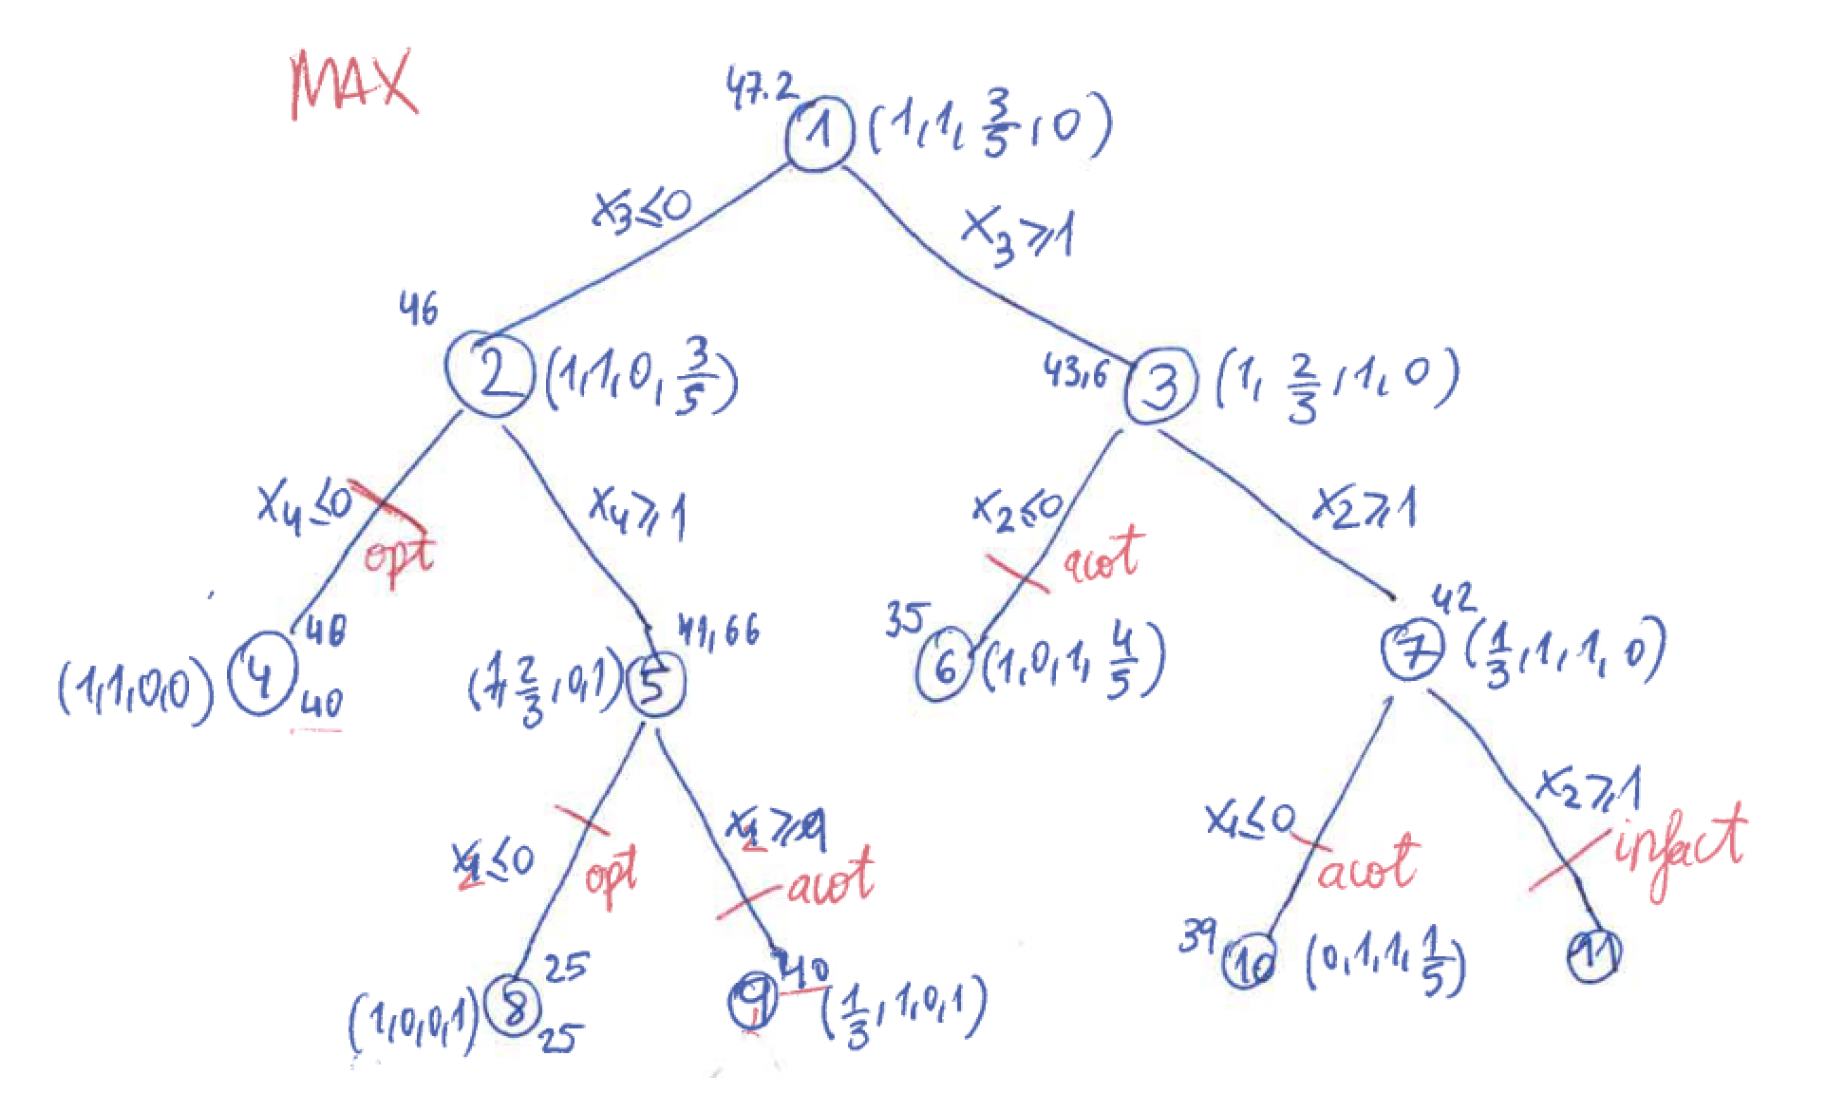
\includegraphics[width=15cm]{ejercicios/BandB01_sol.png}
    %\caption{Caption}
    %\label{fig:enter-label}
\end{figure}
\clearpage
\section{BandB PE3}
\input{ejercicios/BandB_PE3}
\subsection*{Solución}
Se quiere resolver el siguiente problema de programación lineal mediante el algoritmo de \textit{Branch \& Bound} propuesto por Dakin:

\begin{equation}
\begin{split}
\mbox{max. } z = 3x_1 + 5x_2\\
s.a.:\\
2x_1 + 4x_2 \leq  25\\
x_1 \leq 8\\
2x_2 \leq 10\\
x_1,\,\,x_2 \in  \mathcal{Z}^+
\end{split}
\end{equation}

Se ha generado este árbol.


\begin{figure}[h!]
    \begin{center}
    \begin{tikzpicture}[->,>=stealth',level/.style={sibling distance = 5cm/#1,
      level distance = 1.5cm}, scale=1.5] 
    \node [arn_n, label=right: \tiny{$x^*_{RL_0}$=(8, 2.25)}, label=above right: \textbf{\tiny{}}] {\tiny{$P_{0}$}}
        child{ node [arn_n, label=right: \tiny{}, label=below left: \textbf{\tiny{}}, label=above left: \textbf{\tiny{}}, label=below left: \textbf{\tiny{$\underline{z}_1$=420}}] {\tiny{$P_{1}$} }
            edge from parent node[above left] {}
        	}
        child{ node [arn_n, label=right: \tiny{$x^*_{RL_2}$=(6.5, 3)}, label=below right: \textbf{\tiny{}}, label=above right: \textbf{\tiny{}}] {\tiny{$P_{2}$}} 
            child{ node [arn_n, label=above left:\textbf{\tiny{$\overline{z}_3$=34.25}}, label=right: \tiny{}, label=below right: \textbf{\tiny{}}] {\tiny{$P_{3}$}}
                child{ node [arn_n, label=above right:\textbf{\tiny{}}, label=right: \tiny{$x^*_{RL_5}$=(6, 3)}, label=below right: \textbf{\tiny{}}] {\tiny{$P_{5}$}} edge from parent node[above left] {}
                }
                child{ node [arn_n, label=above right:\textbf{\tiny{}}, label=right: \tiny{$x^*_{RL_6}$=(4.5, 4)}, label=below right: \textbf{\tiny{}}] {\tiny{$P_{6}$}} edge from parent node[above right] {}
                }
            edge from parent node[above left] {}
                }
            child{ node [arn_n, label= right:\tiny{}, label=above right:\textbf{\tiny{}}, label=below right: \textbf{\tiny{}}] {\tiny{$P_{4}$}} edge from parent node[above right] {}
                }
        edge from parent node[above right] {}
    		}
    ; 
    \end{tikzpicture}
    \end{center}
\end{figure}

Se pide actualizar las cotas de cada nodos del árbol e indica, en su caso, si se tiene que estudiar o ramificar.

--

En este árbol se actualizan las cotas:
\begin{figure}[h!]
    \begin{center}
    \begin{tikzpicture}[->,>=stealth',level/.style={sibling distance = 5cm/#1,
      level distance = 1.5cm}, scale=1.5] 
    \node [arn_n, label=right: \tiny{$x^*_{RL_0}$=(8, 2.25)}, label=above right: \textbf{\tiny{34}}, label=below right:\textbf{\tiny{34}}] {\tiny{$P_{0}$}}
        child{ node [arn_n, label=right: \tiny{(8,2)}, label=below left: \textbf{\tiny{34}}, label=above left: \textbf{\tiny{34}}, label=below left: \textbf{\tiny{34}}] {\tiny{$P_{1}$} }
            edge from parent node[above left] {}
        	}
        child{ node [arn_n, label=right: \tiny{$x^*_{RL_2}$=(6.5, 3)}, label=below right: \textbf{\tiny{33}}, label=above right: \textbf{\tiny{33.5}}] {\tiny{$P_{2}$}} 
            child{ node [arn_n, label=above left:\textbf{\tiny{33.5}}, label=right: \tiny{}, label=below left: \textbf{\tiny{33}}] {\tiny{$P_{3}$}}
                child{ node [arn_n, label=above right:\textbf{\tiny{33}}, label=right: \tiny{$x^*_{RL_5}$=(6, 3)}, label=below right: \textbf{\tiny{33}}] {\tiny{$P_{5}$}} edge from parent node[above left] {}
                }
                child{ node [arn_n, label=above right:\textbf{\tiny{33.5}}, label=right: \tiny{$x^*_{RL_6}$=(4.5, 4)}, label=below right: \textbf{\tiny{}}] {\tiny{$P_{6}$}} edge from parent node[above right] {}
                }
            edge from parent node[above left] {}
                }
            child{ node [arn_n, label= right:\tiny{no factible}, label=above right:\textbf{\tiny{}}, label=below right: \textbf{\tiny{}}] {\tiny{$P_{4}$}} edge from parent node[above right] {}
                }
        edge from parent node[above right] {}
    		}
    ; 
    \end{tikzpicture}
    \end{center}
\end{figure}

Acción en cada nodo:
\begin{itemize}
    \item Nodo P1: Se poda por optimalidad, se ha obtenido una cota inferior.
    \item Nodo P4: Se tiene que estudiar. El subproblema P4 no es factible.
    \item Nodo P5: Se poda por optimalidad, se ha obtenido una cota inferior.
    \item Nodo P6: Se poda por acotamiento ($z^*_{P6}\leq z^*_{P1}$)
\end{itemize}
La $x^*_{PE}=(8,2)$ con $x^*_{PE}=34$.
\clearpage
\section{BandB sin restricciones}
A continuación se presenta un árbol que se ha obtenido al aplicar el algoritmo de \textit{Branch and Bound} de Dakin a un problema de maximizar con dos variables de decisión: $x_1$ y $x_2$.

Cuando se ha obtenido la solución óptima de la relajación lineal de un nodo se indica el valor de la función objetivo y la de la variables de esa solución.


\begin{figure}[h!]
    \begin{center}
    \begin{tikzpicture}[->,>=stealth',level/.style={sibling distance = 5cm/#1,
      level distance = 1.5cm}] 
    \node [arn_n, label=right: \tiny{(3.571, 3.429)}, label=above right: \textbf{\tiny{440}}] {\tiny{$P_{0}$}}
        child{ node [arn_n, label=right: \tiny{(3, 4)}, label=below left: \textbf{\tiny{}}, label=above left: \textbf{\tiny{420}}, label=below left: \textbf{\tiny{}}] {\tiny{$P_{1}$} }
            edge from parent node[above left] {$x_1 \leq 3$}
        	}
        child{ node [arn_n, label=right: \tiny{(4, 2.4)}, label=below right: \textbf{\tiny{}}, label=above right: \textbf{\tiny{428}}] {\tiny{$P_{2}$}} 
            child{ node [arn_n, label=above left:\textbf{\tiny{423.3}}, label=right: \tiny{(4.1, 2)}, label=below right: \textbf{\tiny{}}] {\tiny{$P_{3}$}}
                child{ node [arn_n, label=above right:\textbf{\tiny{410}}, label=right: \tiny{(4, 2)}, label=below right: \textbf{\tiny{}}] {\tiny{$P_{5}$}} edge from parent node[above left] {$x_1 \leq 4$}
                }
                child{ node [arn_n, label=above right:\textbf{\tiny{}}, label=right:  , label=below right: \textbf{\tiny{}}] {\tiny{$P_{6}$}} edge from parent node[above right] {$x_1 \geq 5$}
                }
            edge from parent node[above left] {$x_2 \leq 2$}
                }
            child{ node [arn_n, label= right:\tiny{}, label=above right:\textbf{\tiny{}}, label=below right: \textbf{\tiny{}}] {\tiny{$P_{4}$}} edge from parent node[above right] {$x_2\geq 3$}
                }
        edge from parent node[above right] {$x_1 \geq 4$}
    		}
    ; 
    \end{tikzpicture}
    \end{center}
\end{figure}

Se pide:
\begin{enumerate} 
    \item Indicar la mejor cota superior y la mejor cota inferior tanto del problema propuesto como de cada uno de los subproblemas.
    \item Explicar qué nodos y por qué se pueden podar, si es que se pueden podar.
    \item Indicar cuál sería un siguiente paso aplicando el algoritmo de Dakin.
\end{enumerate}

\subsection*{Solución}
\input{ejercicios/BandB_sin restricciones_sol}
\clearpage
\section{BranchAndBound mochila}
El problema de la mochila es un problema clásico de optimización combinatoria en el que se busca seleccionar un subconjunto de elementos que maximice el valor total. Cada artículo tiene un peso  y la suma de todos los pesos no puede exceder el peso máximo de la mochila. En la versión más común, las variables de selección son binarias. Este problema su puede formular así.

\vspace{0.5cm}
Dada una mochila con una capacidad máxima $W$ y un conjunto de $n$ objetos, cada uno con:
\begin{itemize}
    \item peso $w_i$
    \item valor $v_i$ 
\end{itemize}

El objetivo es seleccionar un conjunto de objetos para maximizar el valor total: 
\begin{align*}
\text{max.} \quad & z = \sum_{i=1}^{n} v_i x_i \\
\text{s.a.} \quad & \sum_{i=1}^{n} w_i x_i \leq W \\
                 & x_i \in \{0,1\} \quad \forall i \in \{1, \dots, n\}
\end{align*}


Para resolver la relajación lineal de este problema existe un método \textit{greedy}  que consiste en:
\begin{itemize}
    \item ordenar los objetos en función del valor de $\frac{v_i}{w_i}$ (más prioridad al objeto con mayor valor de $\frac{v_i}{w_i}$)
    \item en orden decreciente del ratio $\frac{v_i}{w_i}$, asignar la mayor cantidad de cada objeto (ahora fraccional) siguiendo el criterio anterior hasta que se utilice toda la capacidad posible.
\end{itemize}

\vspace{1cm}

Resuelve el problema de la mochila con los siguientes datos, utilizando el algoritmo de \textit{Branch\&Bound} y resolviendo los subproblemas mediante el método \textit{greedy} indicado, decidiendo qué nodo elegir según el enfoque \textit{Deep First Node} (o \textit{BackTracking}) resolviendo, en un mismo nivel, primero el subproblema de la izquierda (el subproblema creado con la restricción $\leq$).
\vspace{0.5cm}

\begin{tabular}{|l|c|c|c|c|}
\hline
\textbf{} & \textbf{A} & \textbf{B} & \textbf{C} & \textbf{D} \\
\hline
\textbf{Valor (€)} & 60 & 100 & 240 & 60 \\
\hline
\textbf{Peso (kg)} & 10 & 20 & 30 & 15 \\
\hline
\end{tabular}

Capacidad de la mochila: $W=50$

---

Nota: la solución óptima de la relajación lineal del problema que se pide resolver es $x^*_{RL}=(1,\frac{1}{2},1,0)$ lo que implica hacer uso al completo de la capacidad. Se ha elegido, por orden:
\begin{itemize}
    \item $x_3=1$ que representa un peso de 30kg
    \item $x_1=1$ que representa un peso de 10kg
    \item $x_2=\frac{1}{2}$ que representa un peso de 10kg 
\end{itemize}
\subsection*{Solución}

El objetivo es seleccionar objetos para maximizar el valor total: 
\begin{align*}
\text{max.} \quad & z = \sum_{i=1}^{n} v_i x_i \\
\text{s.a.} \quad & \sum_{i=1}^{n} w_i x_i \leq W \\
                 & x_i \in \{0,1\} \quad \forall i \in \{1, \dots, n\}
\end{align*}


Para resolver la relajación lineal de este problema existe un método \textit{greedy}  que consiste en:
\begin{itemize}
    \item priorizar los objetos en función del valor de $\frac{v_i}{w_i}$ (más prioridad al objeto con mayor valor de $\frac{v_i}{w_i}$)
    \item asignando la mayor cantidad (ahora fraccional) de cada objeto siguiendo el criterio anterior hasta que se utilice toda la capacidad posible.
\end{itemize}

\vspace{1cm}

\textbf{Resuelve el problema de la mochila con los siguientes datos, utilizando el algoritmo de \textit{Branch\&Bound} y resolviendo los subproblemas mediante el método \textit{greedy} indicado, decidiendo qué nodo elegir según el enfoque \textit{Deep First Node} ( o \textit{BackTracking}) resolviendo, en un mismo nivel, primero el subproblema de la izquierda.
\vspace{0.5cm}}

\begin{tabular}{|l|c|c|c|c|}
\hline
\textbf{} & \textbf{A} & \textbf{B} & \textbf{C} & \textbf{D} \\
\hline
\textbf{Valor (€)} & 60 & 100 & 240 & 60 \\
\hline
\textbf{Peso (kg)} & 10 & 20 & 30 & 15 \\
\hline
\end{tabular}

Capacidad de la mochila: $W=50$

---

Nota: La solución óptima de la relajación lineal del problema que se quiere resolver es $z^*_{RL}=(1,\frac{1}{2},1,0)$ utilizando el 100\% de la capacidad disponible. Se ha elegido, por orden:
\begin{itemize}
    \item $x_3=1$ dejando 20 unidades de capacidad disponibles
    \item $x_1=1$ dejando 10 unidades de capacidad disponibles
    \item $x_2=\frac{1}{2}$ dejando 0 unidades de capacidad disponibles

\end{itemize}

\vspace{1cm}
Si para la elección de qué nodo resolver se utiliza el enfoque \textit{Deep First Node} ( o \textit{BackTracking}) y se resuelven, en un mismo nivel, primero el subproblema de la izquierda; el orden de estudio de los subproblemas es: 0, 1, 3, 4, 5, 6, 7, 8 y 2.

El árbol asociado es el siguiente:

\begin{figure}[h!]
    \begin{center}
    \begin{tikzpicture}[
    % Estilo general para los nodos (con círculo y borde)
    node_style/.style={
        draw, % Dibuja el borde del nodo
        circle, % Nodos circulares
        inner sep=2pt, % Espacio interno del nodo
        font=\small % Tamaño de fuente pequeño para el número del nodo
    },
    % Estilo para las etiquetas de las soluciones/vectores en los nodos
    solution_label/.style={
        font=\small, % Fuente pequeña
        align=left, % Alineación a la izquierda
        anchor=west, % Ancla a la izquierda
        inner sep=0pt, % Sin espacio interno adicional
        text width=2.5cm % Ancho del texto para que no se superponga
    },
    % Estilo para las etiquetas de las aristas (variables de decisión)
    edge_label/.style={
        font=\tiny, % Fuente muy pequeña
        auto=right % Posiciona la etiqueta automáticamente a la derecha de la arista
    }
    % El estilo 'pruned_line' no está definido ya que se quitaron las líneas rojas
]

    % Nodo 0 (Raíz)
    \node[node_style] (N0) at (0,0) {0};
    \node[solution_label] at ([xshift=0.3cm]N0.east) {$(1, \frac{1}{2}, 1, 0)$};
    \node[above=0pt of N0, font=\tiny] {350};

    % Rama izquierda desde N0: x2=0
    \node[node_style, below left=2.5cm and 2.5cm of N0] (N1) {1};
    \node[solution_label] at ([xshift=0.3cm]N1.east) {$(1, 0, 1, \frac{2}{3})$};
    \node[above=0pt of N1, font=\tiny] {340};
    \draw[-Stealth] (N0) -- node[edge_label, near start, above] {$x_2=0$} (N1);

    % Rama derecha desde N0: x2=1
    \node[node_style, below right=2.5cm and 2.5cm of N0] (N2) {2};
    \node[solution_label] at ([xshift=0.3cm]N2.east) {$(0, 1, 1, 0)$};
    \node[above=0pt of N2, font=\tiny] {340};
    \node[below=0pt of N2, font=\tiny] {340}; % El 340 de abajo
    \draw[-Stealth] (N0) -- node[edge_label, near start, above] {$x_2=1$} (N2);

    % Rama izquierda desde N1: x4=0
    \node[node_style, below left=2.5cm and 2cm of N1] (N3) {3};
    \node[solution_label] at ([xshift=0.3cm]N3.east) {$(1, 0, 1, 0)$};
    \node[above=0pt of N3, font=\tiny] {300};
    \node[below=0pt of N3, font=\tiny] {300}; % El 300 de abajo
    \draw[-Stealth] (N1) -- node[edge_label, near start, above] {$x_4=0$} (N3);

    % Rama derecha desde N1: x4=1
    \node[node_style, below right=2.5cm and 2cm of N1] (N4) {4};
    \node[solution_label] at ([xshift=0.3cm]N4.east) {$(\frac{1}{2}, 0, 1, 1)$};
    \node[above=0pt of N4, font=\tiny] {330};
    \draw[-Stealth] (N1) -- node[edge_label, near start, above] {$x_4=1$} (N4);

    % Rama izquierda desde N4: x1=0
    \node[node_style, below left=2.5cm and 2cm of N4] (N5) {5};
    \node[solution_label] at ([xshift=0.3cm]N5.east) {$(0, 0, 1, 1)$};
    \node[above=0pt of N5, font=\tiny] {300};
    \node[below=0pt of N5, font=\tiny] {300}; % El 300 de abajo
    \draw[-Stealth] (N4) -- node[edge_label, near start, above] {$x_1=0$} (N5);

    % Rama derecha desde N4: x1=1
    \node[node_style, below right=2.5cm and 2cm of N4] (N6) {6};
    \node[solution_label] at ([xshift=0.3cm]N6.east) {$(1, 0, \frac{5}{6}, 1)$};
    \draw[-Stealth] (N4) -- node[edge_label, near start, above] {$x_1=1$} (N6);

    % Rama izquierda desde N6: x3=0
    \node[node_style, below left=2.5cm and 1.5cm of N6] (N7) {7};
    \node[solution_label] at ([xshift=0.3cm]N7.east) {$(1, 0, 0, 1)$};
    \node[above=0pt of N7, font=\tiny] {120};
    \node[below=0pt of N7, font=\tiny] {120}; % El 120 de abajo
    \draw[-Stealth] (N6) -- node[edge_label, near start, above] {$x_3=0$} (N7);

    % Rama derecha desde N6: x3=1
    \node[node_style, below right=2.5cm and 1.5cm of N6] (N8) {8};
    \node[solution_label] at ([xshift=0.3cm]N8.east) {no factible};
    \draw[-Stealth] (N6) -- node[edge_label, near start, above] {$x_3=1$} (N8);

\end{tikzpicture}
    \end{center}
\end{figure}


La solución óptima del problema entero es $x^*_{PE}=(0,1,1,0)$ con $z^*_{PE}=340$


\clearpage
\section{branchandbound a}

\textbf{Resuelve} el siguiente problema de programación lineal mediante el algoritmo de \textit{Branch \& Bound} propuesto por Dakin:

\begin{equation}
\begin{split}
\mbox{max. } z = 80x_1 + 45x_2\\
s.a.:\\
x_1 + x_2 \leq  7\\
12x_1 + 5x_2 \leq 60\\
x_1,\,\,x_2 \in  \mathcal{Z}^+
\end{split}
\end{equation}

\textit{Nota}: se pueden resolver los diversos subproblemas utilizando el método gráfico o mediante la matriz completa.

% \vspace{1cm}
% \begin{tikzpicture}[scale=1.3]
%     \draw [very thin, gray] (0,0) grid (8,8);
% \end{tikzpicture}

\subsection*{Solución}
\textbf{Resuelve} el siguiente problema de programación lineal mediante el algoritmo de \textit{Branch \& Bound} propuesto por Dakin:

\begin{equation}
\begin{split}
\mbox{max. } z = 80x_1 + 45x_2\\
s.a.:\\
x_1 + x_2 \leq  7\\
12x_1 + 5x_2 \leq 60\\
x_1,\,\,x_2 \in  \mathcal{Z}^+
\end{split}
\end{equation}


La solución óptima es $x^*_{PE}=(3,4)$ con $z^*_{PE}=420$.

A continuación se presenta el árbol que permite llegar a la solución óptima ramificando el nodo inicial por la variable $x_1$ (\textit{lo que ha hecho el 98\% de los alumnos}). Se podía haber hecho ramificando por $x_2$ obteniendo la misma solución óptima. \textit{No se reflejan en éste árbol las cotas actualizadas en ningún nodo}.



\begin{figure}[h!]
    \begin{center}
    \begin{tikzpicture}[->,>=stealth',level/.style={sibling distance = 5cm/#1,
      level distance = 1.5cm}] 
    \node [arn_n, label=right: \tiny{(3.571, 3.429)}, label=above right: \textbf{\tiny{440}}] {\tiny{$P_{0}$}}
        child{ node [arn_r, label=right: \tiny{(3, 4)}, label=below left: \textbf{\tiny{}}, label=above left: \textbf{\tiny{420}}, label=below left: \textbf{\tiny{420}}] {\tiny{$P_{1}$} }
            edge from parent node[above left] {$x_1 \leq 3$}
        	}
        child{ node [arn_n, label=right: \tiny{(4, 2.4)}, label=below right: \textbf{\tiny{}}, label=above right: \textbf{\tiny{428}}] {\tiny{$P_{2}$}} 
            child{ node [arn_n, label=above left:\textbf{\tiny{423.3}}, label=right: \tiny{(4.1, 2)}, label=below right: \textbf{\tiny{}}] {\tiny{$P_{3}$}}
                child{ node [arn_n, label=above right:\textbf{\tiny{410}}, label=right: \tiny{(4, 2)}, label=below right: \textbf{\tiny{410}}] {\tiny{$P_{5}$}} edge from parent node[above left] {$x_1 \leq 4$}
                }
                child{ node [arn_n, label=above right:\textbf{\tiny{400}}, label=right: \tiny{(5, 0)}, label=below right: \textbf{\tiny{400}}] {\tiny{$P_{6}$}} edge from parent node[above right] {$x_1 \geq 5$}
                }
            edge from parent node[above left] {$x_2 \leq 2$}
                }
            child{ node [arn_n, label= right:\tiny{no factible}, label=above right:\textbf{\tiny{}}, label=below right: \textbf{\tiny{}}] {\tiny{$P_{4}$}} edge from parent node[above right] {$x_2\geq 3$}
                }
        edge from parent node[above right] {$x_1 \geq 4$}
    		}
    ; 
    \end{tikzpicture}
    \end{center}
\end{figure}


\clearpage
\section{cargoplan a}
Una empresa de transporte llamada \textbf{CargoPlan} se encarga de distribuir productos en tres zonas diferentes: Zona A, Zona B y Zona C. 
Cada zona tiene una demanda específica y el transporte requiere recursos limitados en términos de combustible y horas de conducción.

Los límites semanales para estos recursos son \textbf{8000 litros de combustible y 3000 horas de conducción}. El beneficio por tonelada transportada a cada zona es de \textbf{50, 40 y 60 euros} para las zonas A, B y C, respectivamente.

Cada tonelada transportada consume los siguientes recursos. Zona A: \textbf{6} litros de combustible y \textbf{3} horas de conducción. Zona B: \textbf{4} litros de combustible y \textbf{2} horas de conducción. Zona C: \textbf{8} litros de combustible y \textbf{5} horas de conducción.

Además, existe un contrato que obliga a transportar al menos \textbf{500 toneladas en total} a las zonas B y C combinadas.


Si $x_1$, $x_2$ y $x_3$ representan las toneladas transportadas semanalmente a las zonas A, B y C, respectivamente, el modelo de programación lineal que permite maximizar el beneficio total es el siguiente:

\begin{equation}
\begin{split}
\mbox{max. } z = 50x_1 + 40x_2 + 60x_3\\
s.a.:\\
6x_1 + 4x_2 + 8x_3 \leq 8000\\
3x_1 + 2x_2 + 5x_3 \leq 3000\\
        x_2 +  x_3 \geq 500\\
x_1,\,\,x_2,\,\,x_3\geq 0\\
\end{split}
\end{equation}

Se dispone de la siguiente tabla, correspondiente a una solución obtenida mediante la aplicación del método del simplex.

\begin{center}
\begin{tabular}{c|c|ccccccc|}
 & $z$ & $x_1$ & $x_2$ & $x_3$ & $h_1$ & $h_2$ & $h_3$ & $a_3$\\ 
 & -60000 & -10 & 0 & -40 & 0 & -20 & 0 & 0 \\ 
\hline
$h_1$ & 2000  & 0 & 0 & -2 & 1 & -2 & 0 & 0\\ 
$h_3$ & 1000  & $3/2$ & 0 & $3/2$ & 0 & $1/2$ & 1 & -1\\ 
$x_2$ & 1500  & $3/2$ & 1 & $5/2$ & 0 & $1/2$ & 0 & 0\\ 
\hline
\end{tabular}
\end{center}





Se pide:

\begin{enumerate}
    \item Interpretar la solución óptima obtenida, incluyendo el beneficio total, la asignación de toneladas transportadas a cada zona y el uso de los recursos disponibles.
\end{enumerate}

Cada una de las preguntas siguientes se refieren a la solución óptima del problema.

\begin{enumerate}
    \setcounter{enumi}{1} % Ajusta el contador para iniciar en 2

    \item Identificar dentro de qué rango podría variar la disponibilidad de combustible (en litros) sin que se modifiquen las variables básicas de la solución óptima y explicar qué cambiaría en la solución el cambio de la disponibilidad de combustible dentro de dicho rango. ¿Cuál sería el plan de transporte fuera de ese rango?

    \item Se ha hecho un análisis del tiempo de conducción en la zona A para reducir el tiempo actual de 3 horas por cada tonelada transportada. ¿Por debajo de qué valor de tiempo de conducción en la zona A sería interesante transportar sus productos a la zona A?

    \item Cuánto estaría dispuesta a pagar la empresa por disponer de una hora adicional de conducción cada semana.

  % \item Cargoplan está renegociando los precios de los clientes de la zona B. Dentro de qué rango de valores del ingreso por tonelada en la zona B se mantendría el plan de distribución.

    \item Evaluar el impacto de relajar o de hacer más restrictivo el contrato que exige transportar al menos 500 toneladas en total a las zonas B y C. En particular, indicar cuánto se podría relajar o cuánto más restrictivo podría ser el acuerdo sin que cambie el plan de distribución óptimo.

    \item Obtener el nuevo plan óptimo de transporte si, por razones logísticas, la empresa decidiera transportar al menos tantas toneladas a la zona A como a la zona C.

    % \item Obtener el nuevo plan óptimo de transporte si, por razones logísticas, la empresa decidiera transportar las mismas cantidades a la zona A que a la zona B.
\end{enumerate}

\subsection*{Solución}
Una empresa de transporte llamada \textbf{CargoPlan} se encarga de distribuir productos en tres zonas diferentes: Zona A, Zona B y Zona C. 
Cada zona tiene una demanda específica y el transporte requiere recursos limitados en términos de combustible y horas de conducción.

Los límites semanales para estos recursos son \textbf{8000 litros de combustible y 3000 horas de conducción}. El beneficio por tonelada transportada a cada zona es de \textbf{50, 40 y 60 euros} para las zonas A, B y C, respectivamente.

Cada tonelada transportada consume los siguientes recursos. Zona A: \textbf{6} litros de combustible y \textbf{3} horas de conducción. Zona B: \textbf{4} litros de combustible y \textbf{2} horas de conducción. Zona C: \textbf{8} litros de combustible y \textbf{5} horas de conducción.

Además, existe un contrato que obliga a transportar al menos \textbf{500 toneladas en total} a las zonas B y C combinadas.


Si $x_1$, $x_2$ y $x_3$ representan las toneladas transportadas semanalmente a las zonas A, B y C, respectivamente, el modelo de programación lineal que permite maximizar el beneficio total es el siguiente:

\begin{equation}
\begin{split}
\nonumber
\mbox{max. } z = 50x_1 + 40x_2 + 60x_3\\
s.a.:\\
6x_1 + 4x_2 + 8x_3 \leq 8000\\
3x_1 + 2x_2 + 5x_3 \leq 3000\\
        x_2 +  x_3 \geq 500\\
x_1,\,\,x_2,\,\,x_3\geq 0\\
\end{split}
\end{equation}

Se dispone de la siguiente tabla, correspondiente a una solución obtenida mediante la aplicación del método del simplex.

\begin{center}
\begin{tabular}{c|c|ccccccc|}
 & $z$ & $x_1$ & $x_2$ & $x_3$ & $h_1$ & $h_2$ & $h_3$ & $a_3$\\ 
 & -60000 & -10 & 0 & -40 & 0 & -20 & 0 & 0 \\ 
\hline
$h_1$ & 2000  & 0 & 0 & -2 & 1 & -2 & 0 & 0\\ 
$h_3$ & 1000  & $3/2$ & 0 & $3/2$ & 0 & $1/2$ & 1 & -1\\ 
$x_2$ & 1500  & $3/2$ & 1 & $5/2$ & 0 & $1/2$ & 0 & 0\\ 
\hline
\end{tabular}
\end{center}


Se pide:

\begin{enumerate}
    \item \textbf{Interpretar la solución óptima obtenida, incluyendo el beneficio total, la asignación de toneladas transportadas a cada zona y el uso de los recursos disponibles.}

    \begin{itemize}
        \item El beneficio es de 60000 euros.
        \item Se envían 1500 toneladas de producto a la zona B y ninguna a las zonas A y C.
        \item No se consumen 2000 de los 8000 litros de combustible disponibles.
        \item Se usan las 3000 horas de conducción al completo.
        \item Se cumple el contrato entregando 1000 unidades más del mínimo acordado (500).
    \end{itemize}
        
    
    
\end{enumerate}

Cada una de las preguntas siguientes se refieren a la solución óptima del problema.

\begin{enumerate}
    \setcounter{enumi}{1} % Ajusta el contador para iniciar en 2

    \item \textbf{Identificar dentro de qué rango podría variar la disponibilidad de combustible (en litros) sin que se modifiquen las variables básicas de la solución óptima y explicar qué cambiaría en la solución el cambio de la disponibilidad de combustible dentro de dicho rango. ¿Cuál sería el plan de transporte fuera de ese rango?}

    \begin{equation}
    \begin{split}
    u^B=B^{-1}b = \begin{pmatrix}
    1 & -2 & 0\\
    0 & 1/2 & -1\\
    0 & 1/2 & 0\\
    \end{pmatrix}
    \begin{pmatrix}
    b_1\\
    3000\\
    500\\
    \end{pmatrix}
     = \begin{pmatrix}
    b_1-6000\\
    1500 - 500\\
    1500\\
    \end{pmatrix}
    \geq 0 \Rightarrow \\
    \left\{
    \begin{array}{l}
    b_1 - 6000 \geq 0 \\
    1000 \geq 0 \\
    1500 \geq 0
    \end{array}
    \right.
    \end{split}
    \end{equation}

    Por lo tanto, $b_1 - 6000 \geq 0 \implies b_1 \geq 6000$ y el intervalo donde se cumplen las tres desigualdades es: $b_1 \in \left[6000, \infty \right)$.
    
    Es decir, siempre y cuando la disponibilidad del combustible sea igual o superior a 6000 litros se mantienen las variables básicas de la solución óptima y se transportaría producto solamente a la zona B.
    
    La variación de la disponibilidad de combustible dentro del rango mencionado haría que solo cambie la cantidad de combustible disponible no utilizado, porque las variables $h_3$ y $x_2$ mantendrían su valor siempre y cuando la disponibilidad de combustible sea igual o superior a 6000 litros. Es decir, en este caso particular, aunque cambia $u^B$ no cambian los valores correspondientes a $x_1$, $x_2$ y $x_3$ y el plan de transporte óptimo se mantiene (lo único que ocurre es que para cualquier valor superior a 6000 para el valor de la disponibilidad de gasolina, cualquier cantidad por encima de dicho valor no se consume).

    Para un valor inferior a 6000, por ejemplo 5999, la solución dejaría de ser factible y habría que aplicar Lemke.

    \begin{center}
    \begin{tabular}{c|c|cccccc|}
     & $z$ & $x_1$ & $x_2$ & $x_3$ & $h_1$ & $h_2$ & $h_3$\\ 
     & $-60000$ & $-10$ & $0$ & $-40$ & $0$ & $-20$ & $0$ \\ 
    \hline
    $h_1$ & -1  & $0$ & $0$ & $-2$ & $1$ & $-2$ & $0$\\ 
    $h_3$ & 1000  & $3/2$ & $0$ & $3/2$ & $0$ & $1/2$ & $1$\\ 
    $x_2$ & 1500  & $3/2$ & $1$ & $5/2$ & $0$ & $1/2$ & $0$\\ 
    \hline
       & $-59990$ & $-10$ & $0$ & $-20$ & $-10$ & $0$ & $0$ \\ 
    \hline
    $h_2$ & 1/2  & $0$ & $0$ & $1$ & $-1/2$ & $1$ & $0$\\ 
    $h_3$ & 3999/4  & $3/2$ & $0$ & $1$ & $1/4$ & $0$ & $1$\\ 
    $x_2$ & 5999/4  & $3/2$ & $1$ & $2$ & $1/4$ & $0$ & $0$\\ 
    \hline
    \end{tabular}
    \end{center}

    En este caso, se seguiría transportando solo a la zona B ($x_2>0$) y nada a las otras dos ($x_1=x_3=0$)), se agotaría todo el combustible ($h_1=0$), no se haría uso de todas las horas de conducción disponibles ($h_2>0$) y se seguiría cumpliendo el compromiso de entregas por encima del valor mínimo acordado ($h_3>0$).    
    
    
    \item \textbf{Se ha hecho un análisis del tiempo de conducción en la zona A para reducir el tiempo actual de 3 horas por cada tonelada transportada. ¿Por debajo de qué valor de tiempo de conducción en la zona A sería interesante transportar sus productos a la zona A?}

    Reducir el tiempo de conducción de la zona significa reducir el valor de $a_{21}$ (actualmente 3). Si cambia $a_{13}$, cambiarían $p_{x_1}$ y $V^B_{x_1}$. En el caso de que $V^B_{x_1} >0$ interesaría transportar toneladas a la zona A.

    \begin{equation}
    \begin{split}
    V^B_{x_1}=c_{x_1}-c^BB^{-1}A_{x_1}=c_{x_1}-\pi^BA_{x_1} = \\
    50 - \begin{pmatrix}
        0 & 20 & 0
    \end{pmatrix}
    \begin{pmatrix}
        6 \\
        a_{21} \\
        0
    \end{pmatrix} = 50 - 20a_{21} > 0 \implies a_{21} < 2.5
    \end{split}
    \end{equation}

    Si el tiempo de conducción de la zona A se redujera por debajo de las 2.5 horas interesaría distribuir en esta zona.   

    \item \textbf{Cuánto estaría dispuesta a pagar la empresa por disponer de una hora adicional de conducción cada semana.}

    El precio sombra de la restricción 2 (conducción) es $\pi_2 = 20$, de forma que cualquier coste inferior a 20 euros por hora adicional de conducción daría lugar a una mejora del beneficio total.

    % \item \textbf{Cargoplan está renegociando los precios de los clientes de la zona B. Dentro de qué rango de valores del ingreso por tonelada en la zona B se mantendría el plan de distribución.}

    % Podemos hacer el análisis de sensibilidad de $c_{x_2}$

    % \begin{equation}
    % \begin{split}
    % V^B = c-c^BB^{-1}A = \begin{pmatrix}
    % 50 & c_{x_2} & 60 & 0 & 0 & 0\\
    % \end{pmatrix}
    %  - \begin{pmatrix}
    % 0 & 0 & c_2\\
    % \end{pmatrix}
    % \begin{pmatrix}
    % 0 & 0 & -2 & 1 & -2 & 0\\
    % 3/2 & 0 & 3/2 & 0 & 1/2 & 1\\
    % 3/2 & 1 & 5/2 & 0 & 1/2 & 0\\
    % \end{pmatrix} = \\
    %  = \begin{pmatrix}
    % 50 & c_{x_2} & 60 & 0 & 0 & 0\\
    % \end{pmatrix} -
    % \begin{pmatrix}
    % 3/2c_{x_2} & c_{x_2} & 5/2c_{x_2}& 0 & 1/2c_{x_2} & 0\\
    % \end{pmatrix} = \\
    % \begin{pmatrix}
    % 50- 3/2c_{x_2} & 0 & 60 - 5/2c_{x_2}& 0 & -1/2c_{x_2} & 0\\
    % \end{pmatrix}
    % \end{split}
    % \end{equation}

    % Para que la solución siga siendo óptima se debe cumplir $V^B\leq 0$:

    % \begin{equation}
    %     \left.
    %     \begin{matrix}
    %     50- 3/2c_{x_2} \leq 0 \implies c_{x_2} \geq 100/3\\
    %     60 - 5/2c_{x_2} \leq 0 \implies c_{x_2} \geq 24\\
    %     -1/2c_{x_2} \leq 0 \leq 0 \implies c_{x_2} \geq 0\\
    %     \end{matrix}
    %     \right\} \implies c_{x_2} \geq 100/3
    % \end{equation}

    % Siempre y cuando el ingreso por tonelada de la zona B sea igual o superior a $\frac{100}{3}$ el plan de distribución seguirá siendo óptimo.

    \item \textbf{Evaluar el impacto de relajar o de hacer más restrictivo el contrato que exige transportar al menos 500 toneladas en total a las zonas B y C. En particular, indicar cuánto se podría relajar o cuánto más restrictivo podría ser el acuerdo sin que cambie el plan de distribución óptimo.}

    CargoPlan está cumpliendo el compromiso comercial por encima del mínimo acordado, por lo que no tiene incentivo en relajarlo y, por otro lado, hacerlo más restrictivo salvo que hubiera que entregar más de 1500 unidades entre las zonas B y C.

    Los valores de las variables básicas cambian con el cambio de $b_3$:

    \begin{equation}
    u^B=B^{-1}b = \begin{pmatrix}
    1 & -2 & 0\\
    0 & 1/2 & -1\\
    0 & 1/2 & 0\\
    \end{pmatrix}
    \begin{pmatrix}
    8000\\
    3000\\
    b_3\\
    \end{pmatrix}
     = \begin{pmatrix}
    2000\\
    1500 - b_3\\
    1500\\
    \end{pmatrix}
    \end{equation}

        Si el compromiso comercial no excede 1500 unidades, es decir, $b_3 \in (-\infty, 1500]$, la base de la tabla original sigue conduciendo a la solución óptima.

        La variación del compromiso de comercial dentro del rango mencionado haría que solo cambie la cantidad en la que se excede el compromiso comercial, porque las variables $x_2$ y $h_1$ dentro de dicho intervalo. Es decir, en este caso particular, aunque cambia $u^B$ no cambian los valores correspondientes a $x_1$, $x_2$ y $x_3$ y el plan de transporte óptimo se mantiene (lo único que ocurre es que para cualquier valor inferior a 1500 se excederá el compromiso comercial en diferente cuantía según el valor de aquel).

    \item \textbf{Obtener el nuevo plan óptimo de transporte si, por razones logísticas, la empresa decidiera transportar al menos tantas toneladas a la zona A como a la zona C.}

    El plan de producción cumple con el requisito y sigue siendo factible y también óptimo.

    % \item Obtener el nuevo plan óptimo de transporte si, por razones logísticas, la empresa decidiera transportar las mismas cantidades a la zona A que a la zona B.
    
%     El nuevo requisito se traduciría en la aparición de una nueva restricción: $x_1=x_2$, equivalente a $x_1 - x_2 = 0$, a su vez, equivalente a añadir dos restricciones; $x_1 - x_2 \leq 0$ y $x_1 - x_2 \geq 0$, que se pueden formular en términos de igualdad añadiendo las correspondientes variables de holgura: $x_1 - x_2 + h_4 = 0$ y $x_1 - x_2 - h_5 = 0$

%     \begin{center}
%     \begin{tabular}{c|c|cccccccc|}
%      & $z$ & $x_1$ & $x_2$ & $x_3$ & $h_1$ & $h_2$ & $h_3$ & $h_4$ & $h_5$\\ 
%      & -60000 & -10 & 0 & -40 & 0 & -20 & 0 & 0 & 0\\ 
%     \hline
%     $h_1$ & 2000  & 0 & 0 & -2 & 1 & -2 & 0 & 0 & 0\\ 
%     $h_3$ & 1000  & $3/2$ & 0 & $3/2$ & 0 & $1/2$ & 1 & 0 & 0\\ 
%     $x_2$ & 1500  & $3/2$ & 1 & $5/2$ & 0 & $1/2$ & 0 & 0 & 0\\ 
%     \hline
%           &    0  &     1 &-1 &     0 & 0 &     0 & 0 & 1 & 0\\ 
%           &    0  &     1 &-1 &     0 & 0 &     0 & 0 & 0 & -1\\ 
%     \hline
%     $h_4$ & 1500  &   5/2 & 0 &   5/2 & 0 &   1/2 & 0 & 1 & 0\\ 
%     $h_5$ & -1500 &  -5/2 & 0 &  -5/2 & 0 &  -1/2 & 0 & 0 & 1\\ 
%     \hline
%      & $z$ & $x_1$ & $x_2$ & $x_3$ & $h_1$ & $h_2$ & $h_3$ & $h_4$ & $h_5$\\ 
%      & -60000 & -10 & 0 & -40 & 0 & -20 & 0 & 0 & 0\\ 
%     \hline
%     $h_1$ & 2000  & 0 & 0 & -2 & 1 & -2 & 0 & 0 & 0\\ 
%     $h_3$ & 1000  & $3/2$ & 0 & $3/2$ & 0 & $1/2$ & 1 & 0 & 0\\ 
%     $x_2$ & 1500  & $3/2$ & 1 & $5/2$ & 0 & $1/2$ & 0 & 0 & 0\\ 
%     $h_4$ & 1500  &   5/2 & 0 &   5/2 & 0 &   1/2 & 0 & 1 & 0\\ 
%     $h_5$ & -1500 &  -5/2 & 0 &  -5/2 & 0 &  -1/2 & 0 & 0 & 1\\ 
%     \hline
%  & -54000 & 0 & 0 & -30 & 0 & -18 & 0 & 0 & -4 \\ 
% \hline
% $h_1$ & 2000  & 0 & 0 & -2 & 1 & -2 & 0 & 0 & 0\\ 
% $h_3$ & 100  & 0 & 0 & 0 & 0 & $1/5$ & 1 & 0 & $3/5$\\ 
% $x_2$ & 600  & 0 & 1 & 1 & 0 & $1/5$ & 0 & 0 & $3/5$\\ 
% $h_4$ & 0  & 0 & 0 & 0 & 0 & 0 & 0 & 1 & 1\\ 
% $x_1$ & 600  & 1 & 0 & 1 & 0 & $1/5$ & 0 & 0 & $-2/5$\\ 
% \hline
% \end{tabular}
% \end{center}

% De acuerdo con la tabla de la solución óptima tras aplicar el método de Lemke, la nueva solución óptima se caracteriza por lo siguiente.
%     \begin{itemize}
%         \item El beneficio es de 54000 euros (6000 menos que antes de imponer el requisito).
%         \item Se envían 600 toneladas de producto a la zona B y otras tantas a la zona A, y ninguna a la zona C.
%         \item No se consumen 2000 de los 8000 litros de combustible disponibles.
%         \item Se usan las 3000 horas de conducción al completo.
%         \item Se cumple el contrato entregando 100 unidades más del mínimo acordado (500).
%     \end{itemize}
        

     
\end{enumerate}
\clearpage
\section{cartero chino}
Un ayuntamiento es responsable de mantener la siguiente red de carreteras. El número en cada arista es la longitud de la carretera en kilómetros.

\vspace{0.5cm} % Espacio vertical para separar el texto del gráfico

\begin{center}
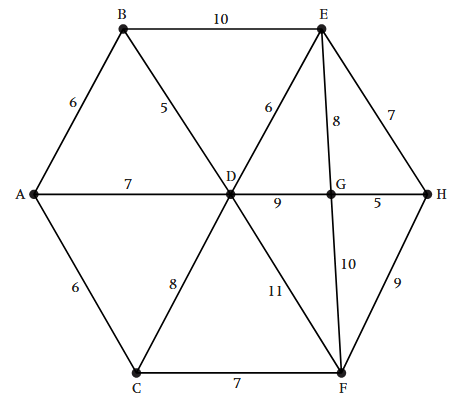
\includegraphics{ejercicios/carreteras_estado.png}

\end{center}

\vspace{0.5cm} % Espacio vertical

La oficina del ayuntamiento está ubicada en A.

\textbf{(a)} Un trabajador del ayuntamiento tiene que inspeccionar todas las carreteras, empezando y terminando en A. Encuentre la longitud de una ruta óptima.

\vspace{0.5cm} 

\textbf{(b)} Un supervisor, con base en A, también desea inspeccionar todas las carreteras. Sin embargo, el supervisor vive en H y desea comenzar su ruta en A y terminar en H. Encuentre la longitud de una ruta óptima para el supervisor.


\subsection*{Solución}
Un ayuntamiento es responsable de mantener la siguiente red de carreteras. El número en cada arista es la longitud de la carretera en kilómetros.

\vspace{0.5cm} % Espacio vertical para separar el texto del gráfico

\begin{center}
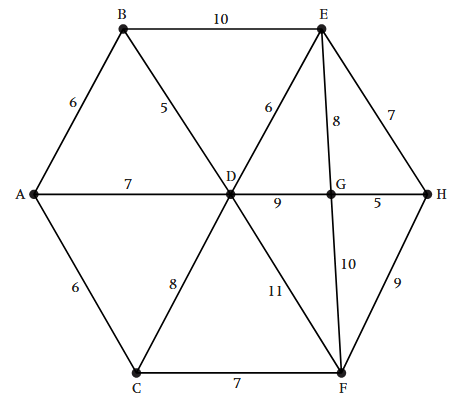
\includegraphics{ejercicios/carreteras_estado.png}

\end{center}

\vspace{0.5cm} % Espacio vertical

La oficina del ayuntamiento está ubicada en A.

\textbf{(a)} Un trabajador del ayuntamiento tiene que inspeccionar todas las carreteras, empezando y terminando en A. Encuentre la longitud de una ruta óptima.

\vspace{0.5cm} 

\textbf{(b)} Un supervisor, con base en A, también desea inspeccionar todas las carreteras. Sin embargo, el supervisor vive en H y desea comenzar su ruta en A y terminar en H. Encuentre la longitud de una ruta óptima para el supervisor.

\vspace{0.5cm}
\textbf{Solución}
\vspace{0.5cm}

\textbf{(a)} Hay cuatro vértices de grado impar: A, B, C y H.
Hay tres formas de emparejar estos vértices impares y la longitud mínima de cada emparejamiento es:
\begin{align*}
\text{AB + CH} &= 6 + 16 = 22 \\
\text{AC + BH} &= 6 + 17 = 23 \\
\text{AH + BC} &= 21 + 12 = 33
\end{align*}

La longitud de todas las carreteras en la red es 116.
La longitud de una ruta óptima del cartero chino para el trabajador es $116 + 22 = 138$ kilómetros.

\vspace{1cm} 

\textbf{(b)} Comenzar en A y terminar en H deja dos vértices de grado impar: B y C (que hay que unir).
La distancia mínima de B a C es 12.
Si empieza el camino en A acabará en H con una distancia de $116 + 12 = 128$ kilómetros.
\clearpage
\section{convex hull}
En la siguiente figura se indican las cuatro restricciones de un problema de programación lineal entera:

\begin{figure}[h!]
    \centering
    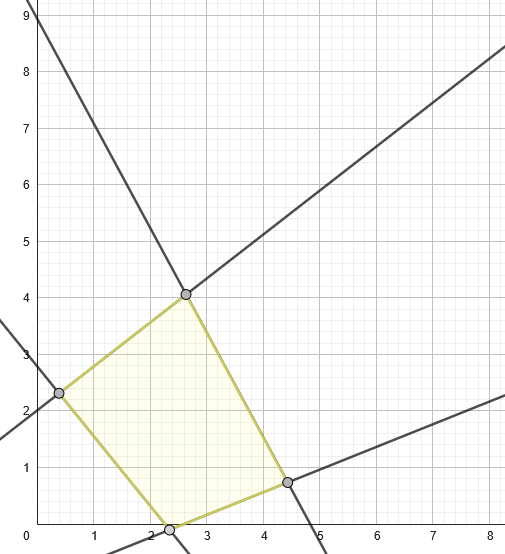
\includegraphics[width=10cm]{ejercicios/convex_hull_enunciado.png} 
\end{figure}

Formula las restricciones que generan el \textit{convex hull} (o envolvente convexa) de este problema.

\subsection*{Solución}

En la siguiente figura se muestran las 8 soluciones enteras y el polígono (líneas en puntitos) correspondiente al convex hull.

Las restricciones que generan la envolvente convexa son:

\begin{itemize}
    \item $x_2 \leq 3$
    \item $2x_1+x_2 \leq 9$
    \item $x_2 \geq 1$
    \item $x_1+x_2 \geq 3$
    \item $-x_1+x_2 \leq 1$
\end{itemize}

\begin{figure}[h!]
    \centering
    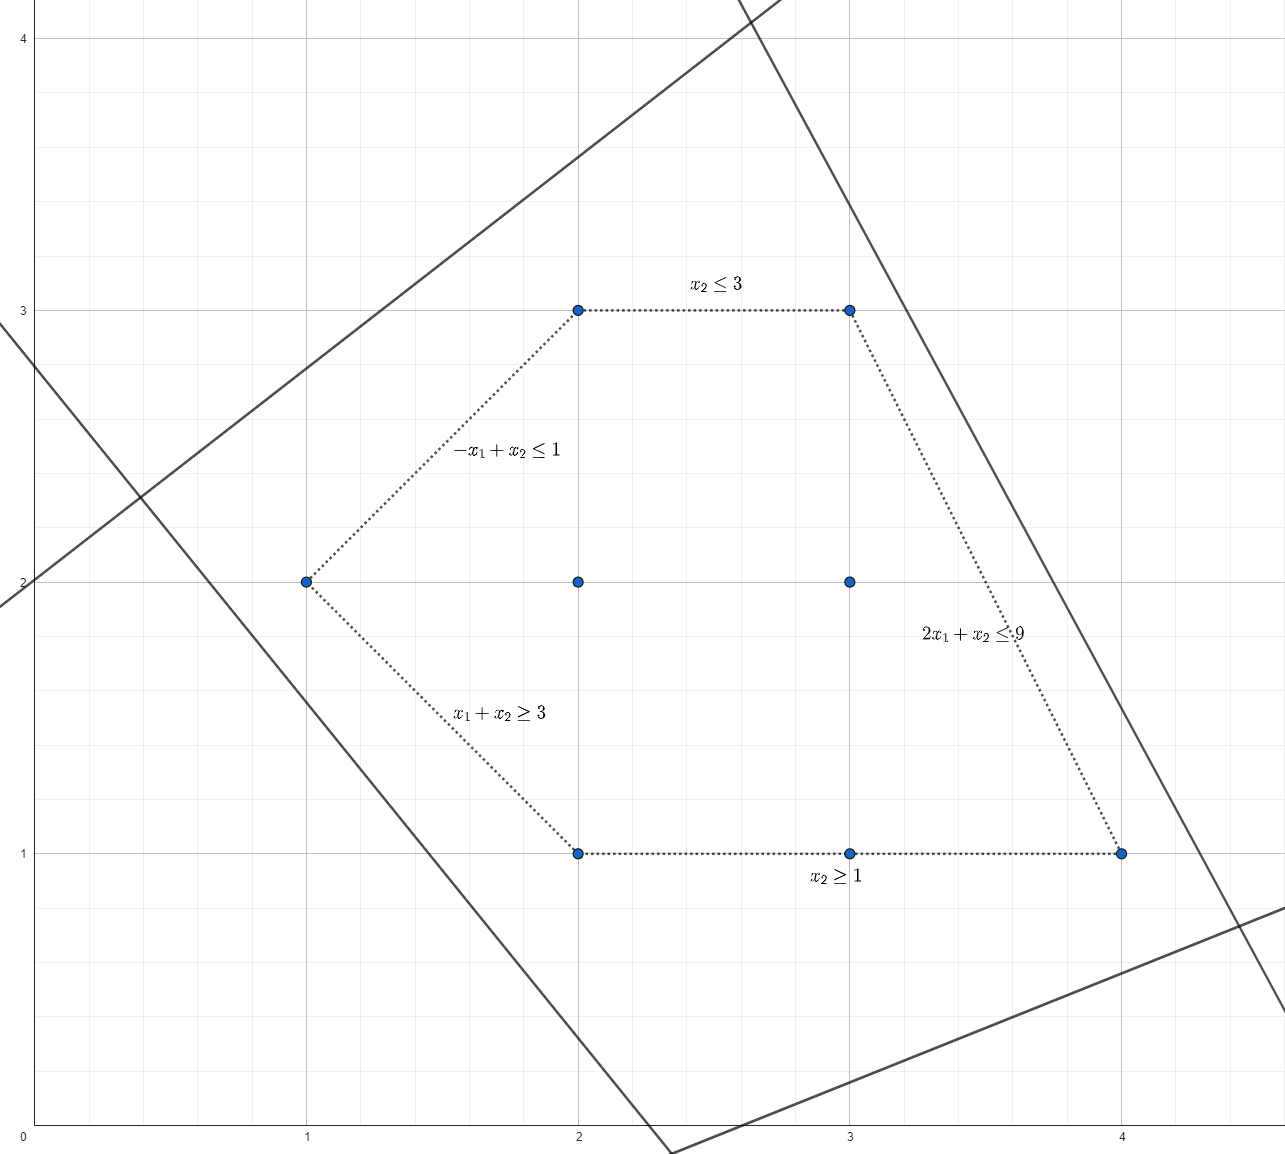
\includegraphics[width=10cm]{ejercicios/convex_hull_solucion.png} 
    %\includesvg[width=0.8\textwidth]{ejercicios/convex_hull.svg}
    %\caption{Descripción de tu gráfico SVG.}
    \label{fig:mi_grafico_svg}
\end{figure}
\clearpage
\section{degenerada optima multiple primal dual}

Dado el siguiente problema de programación lineal:

\begin{equation}
\begin{split}
\mbox{max. } z = 3x_1 + 2x_2\\
s.a.:\\
2x_1 + 4x_2 \leq 80\\
4x_1 + 3x_2 \leq 60\\
 x_1 +  x_2 \leq 15\\
x_1,\,\,x_2\geq 0\\
\end{split}
\end{equation}

Se conoce la solución óptima.

\begin{center}
\begin{tabular}{c|c|ccccc|}
 & $z$ & $x_1$ & $x_2$ & $h_1$ & $h_2$ & $h_3$\\ 
 & -45 & 0 & -1/4 & 0 & -3/4 & 0 \\ 
\hline
$h_1$ & 50  & 0 & 5/2 & 1 & -1/2 & 0\\ 
$x_1$ & 15  & 1 & 3/4 & 0 & 1/4 & 0\\ 
$h_3$ & 0  & 0 & 1/4 & 0 & -1/4 & 1\\ 
\hline
\end{tabular}
\end{center}



\begin{enumerate}
    \item Se pide formular el problema dual asociado.

\item Dada la siguiente tabla, que corresponde a una solución óptima del problema dual asociado, comprobar que se cumple el teorema fundamental de la dualidad entre el problema primal y el problema dual y, sus respectivas soluciones óptimas. 

\begin{center}
\begin{tabular}{c|c|ccccc|}
 & $z$ & $y_1$ & $y_2$ & $y_3$ & $h_1$ & $h_2$\\ 
 & 45 & -50 & 0 & 0 & -15 & 0 \\ 
\hline
$h_2$ & 1  & -2 & 1 & 0 & -1 & 1\\ 
$y_3$ & 3  & 2 & 4 & 1 & -1 & 0\\ 
\hline
\end{tabular}
\end{center}

\end{enumerate}     
\subsection*{Solución}
El problema dual tiene la forma:

\begin{equation}
\begin{split}
\mbox{min. } z = 80y_1 + 60y_2 + 15y_3\\
\mbox{max. } z = - 80y_1 - 60y_2 - 15y_3\\
s.a.:\\
2y_1 + 4y_2 + y_3 \geq 3\\
4y_1 + 3y_2 + y_3 \geq 2\\
y_1,\,\,y_2,\,\,y_3\geq 0\\
\end{split}
\end{equation}

La solución del dual es una solución óptima múltiple y, aplicando el método del simplex, se puede obtener una solución óptima alternativa:

\begin{center}
\begin{tabular}{c|c|ccccc|}
 & $z$ & $y_1$ & $y_2$ & $y_3$ & $h_1$ & $h_2$\\ 
 Base 1 & 45 & -50 & 0 & 0 & -15 & 0 \\ 
\hline
$h_2$ & 1  & -2 & 1 & 0 & -1 & 1\\ 
$x_3$ & 3  & 2 & 4 & 1 & -1 & 0\\ 
\hline
Base 2  & 45 & -50 & 0 & 0 & -15 & 0 \\ 
\hline
$h_2$ & 1/4  & $\frac{-5}{2}$ & 0 & $\frac{-1}{4}$ & $\frac{-3}{4}$ & 1\\ 
$y_2$ & 3/4  & $\frac{1}{2}$ & 1 & $\frac{1}{4}$ & $\frac{-1}{4}$ & 0\\ 
\hline
\end{tabular}
\end{center}




% \begin{center}
% \begin{tabular}{c|c|ccccccc|}
%   & $z$ & $y_1$ & $y_2$ & $y_3$ & $h_1$ & $h_2$ & $a_1$ & $a_2$\\ 
% Base 1 & 45 & -50 & 0 & 0 & -15 & 0 & 15 & 0 \\ 
% \hline
% $h_2$ & 1  & -2 & 1 & 0 & -1 & 1 & 1 & -1\\ 
% $y_3$ & 3  & 2 & 4 & 1 & -1 & 0 & 1 & 0\\ 
% \hline
% Base 2 & 45 & -50 & 0 & 0 & -15 & 0 & 15 & 0 \\ 
% \hline
% $h_2$ & 1/4  & -5/2 & 0 & -1/4 & -3/4 & 1 & 3/4 & -1\\ 
% $y_2$ & 3/4  & 1/2 & 1 & 1/4 & -1/4 & 0 & 1/4 & 0\\ 
% \hline
% \end{tabular}
% \end{center}
% \begin{center}
% \begin{tabular}{c|c|ccccccc|}
 % & $z$ & $y_1$ & $y_2$ & $y_3$ & $h_1$ & $h_2$ & $a_1$ & $a_2$\\ 

% \end{tabular}
% \end{center}


Por su parte, la solución del problema primal es una solución degenerada y, aplicando lemke, se puede obtener la misma solución con una base diferente:


\begin{center}
\begin{tabular}{c|c|ccccc|}
 & $z$ & $x_1$ & $x_2$ & $h_1$ & $h_2$ & $h_3$\\ 
Base 2 & -45 & 0 & -1/4 & 0 & -3/4 & 0 \\ 
\hline
$h_1$ & 50  & 0 & 5/2 & 1 & -1/2 & 0\\ 
$x_1$ & 15  & 1 & 3/4 & 0 & 1/4 & 0\\ 
$h_3$ & 0  & 0 & 1/4 & 0 & -1/4 & 1\\ 
\hline
Base 1 & -45 & 0 & -1 & 0 & 0 & -3 \\ 
\hline
$h_1$ & 50  & 0 & 2 & 1 & 0 & -2\\ 
$x_1$ & 15  & 1 & 1 & 0 & 0 & 1\\ 
$h_2$ & 0  & 0 & -1 & 0 & 1 & -4\\ 
\hline
\end{tabular}
\end{center}


La solución con la base 1 del primal se corresponde con la base 2 del dual, y se cumple el teorema fundamental de la dualidad ($y_1^*=\pi^B_1=0$, $y_2^*=\pi^B_2=0$,  $y_3^*=\pi^B_3=3$). Igualmente, La solución con la base 2 del primal se corresponde con la base 1 del dual, y se cumple el teorema fundamental de la dualidad ($y_1^*=\pi^B_1=0$, $y_2^*=\pi^B_2=3/4$, $y_3^*=\pi^B_3=0$)



\clearpage
\section{demo dieta}
Una dieta debe aportar al menos 80 unidades de proteína usando dos alimentos
$x_1$ y $x_2$, sin superar 60 unidades de grasa. Cada unidad de $x_1$ aporta 2 de
proteína y 4 de grasa; cada unidad de $x_2$, 4 de proteína y 3 de grasa. Los
costes unitarios son 3 y 2. El modelo que minimiza el coste es:

\begin{equation}
\begin{split}
\label{eq:demo_dieta}
\mbox{min. } z = 3x_1 + 2x_2\\
s.a.:\\
2x_1 + 4x_2 \geq 80\\
4x_1 + 3x_2 \leq 60\\
x_1,\,\,x_2\geq 0\\
\end{split}
\end{equation}

\begin{enumerate}
    \item Resolver el problema mediante el método de Lemke.
\end{enumerate}

\subsection*{Solución}
\begin{center}
\begin{tabular}{c|c|cccc|}
 & $z$ & $x_1$ & $x_2$ & $h_1$ & $h_2$\\ 
Fase 2 & $0$ & $-3$ & $-2$ & $0$ & $0$ \\ 
\hline
$h_1$ & $-80$  & $-2$ & $-4$ & $1$ & $0$\\ 
$h_2$ & $60$  & $4$ & $3$ & $0$ & $1$\\ 
\hline
Fase 2 & $40$ & $-2$ & $0$ & $\frac{-1}{2}$ & $0$ \\ 
\hline
$x_2$ & $20$  & $\frac{1}{2}$ & $1$ & $\frac{-1}{4}$ & $0$\\ 
$h_2$ & $0$  & $\frac{5}{2}$ & $0$ & $\frac{3}{4}$ & $1$\\ 
\hline
\end{tabular}
\end{center}


\clearpage
\section{demo muebles}
Un taller fabrica \textbf{mesas} ($x_1$) y \textbf{sillas} ($x_2$). Cada mesa deja
un beneficio de 5 u.m. y cada silla de 4 u.m. La carpintería dispone de 18 horas
y el acabado de 12 horas; una mesa consume 3 horas de carpintería y 1 de acabado,
y una silla 2 y 2 respectivamente. Por contrato deben fabricarse al menos 2 mesas.
El modelo que maximiza el beneficio es el siguiente:

\begin{equation}
\begin{split}
\label{eq:demo_muebles}
\mbox{max. } z = 5x_1 + 4x_2\\
s.a.:\\
3x_1 + 2x_2 \leq 18\\
1x_1 + 2x_2 \leq 12\\
1x_1 \geq 2\\
x_1,\,\,x_2\geq 0\\
\end{split}
\end{equation}

\begin{enumerate}
    \item Formular el problema de la primera fase del método de las dos fases.
    \item Resolver el problema mediante el método de la matriz completa.
    \item Indicar el plan de producción óptimo y el beneficio alcanzado.
\end{enumerate}

\subsection*{Solución}
\begin{equation}
\begin{split}
\mbox{max. } z' = -1a_3\\
s.a.:\\
3x_1+2x_2+1h_1 = 18\\
1x_1+2x_2+1h_2 = 12\\
1x_1-1h_3+1a_3 = 2\\
x_1,\,x_2,\,h_1,\,h_2,\,h_3,\,a_3\geq 0\end{split}
\end{equation}

\begin{center}
\begin{tabular}{c|c|cccccc|}
 & $z$ & $x_1$ & $x_2$ & $h_1$ & $h_2$ & $h_3$ & $a_3$\\ 
Fase 1 & $2$ & $1$ & $0$ & $0$ & $0$ & $-1$ & $0$ \\ 
Fase 2 & $0$ & $5$ & $4$ & $0$ & $0$ & $0$ & $0$ \\ 
\hline
$h_1$ & $18$  & $3$ & $2$ & $1$ & $0$ & $0$ & $0$\\ 
$h_2$ & $12$  & $1$ & $2$ & $0$ & $1$ & $0$ & $0$\\ 
$a_3$ & $2$  & $1$ & $0$ & $0$ & $0$ & $-1$ & $1$\\ 
\hline
Fase 1 & $0$ & $0$ & $0$ & $0$ & $0$ & $0$ & $-1$ \\ 
Fase 2 & $-10$ & $0$ & $4$ & $0$ & $0$ & $5$ & $-5$ \\ 
\hline
$h_1$ & $12$  & $0$ & $2$ & $1$ & $0$ & $3$ & $-3$\\ 
$h_2$ & $10$  & $0$ & $2$ & $0$ & $1$ & $1$ & $-1$\\ 
$x_1$ & $2$  & $1$ & $0$ & $0$ & $0$ & $-1$ & $1$\\ 
\hline
Fase 2 & $-30$ & $0$ & $\frac{2}{3}$ & $\frac{-5}{3}$ & $0$ & $0$ & $0$ \\ 
\hline
$h_3$ & $4$  & $0$ & $\frac{2}{3}$ & $\frac{1}{3}$ & $0$ & $1$ & $-1$\\ 
$h_2$ & $6$  & $0$ & $\frac{4}{3}$ & $\frac{-1}{3}$ & $1$ & $0$ & $0$\\ 
$x_1$ & $6$  & $1$ & $\frac{2}{3}$ & $\frac{1}{3}$ & $0$ & $0$ & $0$\\ 
\hline
Fase 2 & $-33$ & $0$ & $0$ & $\frac{-3}{2}$ & $\frac{-1}{2}$ & $0$ & $0$ \\ 
\hline
$h_3$ & $1$  & $0$ & $0$ & $\frac{1}{2}$ & $\frac{-1}{2}$ & $1$ & $-1$\\ 
$x_2$ & $\frac{9}{2}$  & $0$ & $1$ & $\frac{-1}{4}$ & $\frac{3}{4}$ & $0$ & $0$\\ 
$x_1$ & $3$  & $1$ & $0$ & $\frac{1}{2}$ & $\frac{-1}{2}$ & $0$ & $0$\\ 
\hline
\end{tabular}
\end{center}


\clearpage
\section{dos fases degenerada}
Dado el siguiente problema de Programación Lineal

\begin{equation}
\begin{split}
\mbox{max. } z = 2x_1 + 3x_2\\
s.a.:\\
2x_1 + 3x_2 \leq 40\\
2x_1 + 2x_2 \geq 5\\
2x_2 \geq 5\\
x_1,\,\,x_2\geq 0\\
\end{split}
\end{equation}

Se conoce una tabla correspondiente a la resolución del mismo mediante el método de las dos fases.

\begin{center}
\begin{tabular}{c|c|ccccccc|}
 & $z$ & $x_1$ & $x_2$ & $h_1$ & $h_2$ & $h_3$ & $a_2$ & $a_3$\\ 
Fase 1 & $0$ & $-2$ & $0$ & $0$ & $1$ & $-1$ & $-2$ & $0$ \\
Fase 2 & $-15/2$ & $-1$ & $0$ & $0$ & $3/2$ & $0$ & $-3/2$ & $0$ \\
\hline
$h_1$ & 65/2  & $-1$ & $0$ & $1$ & $3/2$ & $0$ & $-3/2$ & $0$\\
$x_2$ & 5/2  & $1$ & $1$ & $0$ & $-1/2$ & $0$ & $1/2$ & $0$\\
$a_3$ & 0  & $-2$ & $0$ & $0$ & $1$ & $-1$ & $-1$ & $1$\\
\hline
\end{tabular}
\end{center}

Obtener la solución óptima del problema original
\subsection*{Solución}
Dado el siguiente problema de Programación Lineal

\begin{equation}
\begin{split}
\mbox{max. } z = 2x_1 + 3x_2\\
s.a.:\\
2x_1 + 3x_2 \leq 40\\
2x_1 + 2x_2 \geq 5\\
2x_2 \geq 5\\
x_1,\,\,x_2\geq 0\\
\end{split}
\end{equation}

Se conoce una tabla correspondiente a la resolución del mismo mediante el método de las dos fases.

\begin{center}
\begin{tabular}{c|c|ccccccc|}
 & $z$ & $x_1$ & $x_2$ & $h_1$ & $h_2$ & $h_3$ & $a_2$ & $a_3$\\ 
Fase 1 & $0$ & $-2$ & $0$ & $0$ & $1$ & $-1$ & $-2$ & $0$ \\ 
Fase 2 & $-15/2$ & $-59/2$ & $0$ & $0$ & $3/2$ & $0$ & $-3/2$ & $0$ \\ 
\hline
$h_1$ & 65/2  & $-59/2$ & $0$ & $1$ & $3/2$ & $0$ & $-3/2$ & $0$\\ 
$x_2$ & 5/2  & $21/2$ & $1$ & $0$ & $-1/2$ & $0$ & $1/2$ & $0$\\ 
$a_3$ & 0  & $-21$ & $0$ & $0$ & $1$ & $-1$ & $-1$ & $1$\\ 
\hline
\end{tabular}
\end{center}

\noindent \textbf{Obtener la solución óptima del problema original.}
\vspace{0.5cm}

La solución que se ofrece es una solución correspondiente a la primera fase en la que todas las variables artificiales son 0, pero una, $a_3$ es básica, con lo que es posible hacer que otra variable sea básica y que $a_3$ deje de ser básica y, con ello, obtener una solución básica del problema original. 

En la tabla siguiente, por ejemplo, se la elegido que $h_2$ sea variable básica. A partir de ahí, aplicando el método del simplex se obtiene la solución óptima del problema original.

\begin{center}
\begin{tabular}{c|c|ccccccc|}
 & $z$ & $x_1$ & $x_2$ & $h_1$ & $h_2$ & $h_3$ & $a_2$ & $a_3$\\ 
Fase 1 & $0$ & $-2$ & $0$ & $0$ & $1$ & $-1$ & $-2$ & $0$ \\
Fase 2 & $-15/2$ & $-1$ & $0$ & $0$ & $3/2$ & $0$ & $-3/2$ & $0$ \\
\hline
$h_1$ & 65/2  & $-1$ & $0$ & $1$ & $3/2$ & $0$ & $-3/2$ & $0$\\
$x_2$ & 5/2  & $1$ & $1$ & $0$ & $-1/2$ & $0$ & $1/2$ & $0$\\
$a_3$ & 0  & $-2$ & $0$ & $0$ & $1$ & $-1$ & $-1$ & $1$\\
\hline
Fase 1 & $0$ & $0$ & $0$ & $0$ & $0$ & $0$ & $-1$ & $-1$ \\
Fase 2 & $-15/2$ & $2$ & $0$ & $0$ & $0$ & $3/2$ & $0$ & $-3/2$ \\
\hline
$h_1$ & 65/2  & $2$ & $0$ & $1$ & $0$ & $3/2$ & $0$ & $-3/2$\\
$x_2$ & 5/2  & $0$ & $1$ & $0$ & $0$ & $-1/2$ & $0$ & $1/2$\\
$h_2$ & 0  & $-2$ & $0$ & $0$ & $1$ & $-1$ & $-1$ & $1$\\
\hline
Fase 2 & $-40$ & $0$ & $0$ & $-1$ & $0$ & $0$ & $0$ & $0$ \\
\hline
$x_1$ & 65/4  & $1$ & $0$ & $1/2$ & $0$ & $3/4$ & $0$ & $-3/4$\\
$x_2$ & 5/2  & $0$ & $1$ & $0$ & $0$ & $-1/2$ & $0$ & $1/2$\\
$h_2$ & 65/2  & $0$ & $0$ & $1$ & $1$ & $1/2$ & $-1$ & $-1/2$\\
\hline
\end{tabular}
\end{center}
\clearpage
\section{dos fases no acotado a}
\input{ejercicios/dos_fases_no_acotado_a}
\subsection*{Solución}
Dado el siguiente problema de programación lineal:

\begin{equation}
\begin{split}
\mbox{max. } z = 3x_1 + 2x_2 + 4x_3\\
s.a.:\\
2x_1 + 4x_2 - 2x_3 \geq 20\\
 x_1 +  x_2 -  x_3 \leq 80\\
x_1,\,\,x_2,\,\,x_3\geq 0\\
\end{split}
\end{equation}


\begin{enumerate}
    \item Formular el problema equivalente en formato estándar.

    \begin{equation}
    \begin{split}
    \mbox{max. } z = 3x_1 + 2x_2 + 4x_3\\
    s.a.:\\
    2x_1 + 4x_2 - 2x_3 - h_1 = 20\\
     x_1 +  x_2 -  x_3 + h_2 = 80\\
    x_1,\,\,x_2,\,\,x_3,\,h_1,\,h_2\geq 0\\
    \end{split}
    \end{equation}


    \item Formular el problema correspondiente a la primera fase mediante el método de resolución de las dos fases.

\begin{equation}
\begin{split}
\mbox{max. } z' = -a_1\\
s.a.:\\
2x_1+4x_2-2x_3-1h_1+1a_1 = 20\\
1x_1+1x_2-1x_3+1h_2 = 80\\
x_1,\,x_2,\,x_3,\,h_1,\,h_2,\,a_1\geq 0\end{split}
\end{equation}

\item Obtener la solución óptima del problema.


\begin{center}
\begin{tabular}{c|c|cccccc|}
 & $z$ & $x_1$ & $x_2$ & $x_3$ & $h_1$ & $h_2$ & $a_1$\\ 
Fase 1 & 20 & 2 & 4 & -2 & -1 & 0 & 0 \\ 
Fase 2 & 0 & 3 & 2 & 4 & 0 & 0 & 0 \\ 
\hline
$a_1$ & 20  & 2 & 4 & -2 & -1 & 0 & 1\\ 
$h_2$ & 80  & 1 & 1 & -1 & 0 & 1 & 0\\ 
\hline
Fase 1 & 0 & 0 & 0 & 0 & 0 & 0 & -1 \\ 
Fase 2 & -10 & 2 & 0 & 5 & $\frac{1}{2}$ & 0 & $\frac{-1}{2}$ \\ 
\hline
$x_2$ & 5  & $\frac{1}{2}$ & 1 & $\frac{-1}{2}$ & $\frac{-1}{4}$ & 0 & $\frac{1}{4}$\\ 
$h_2$ & 75  & $\frac{1}{2}$ & 0 & $\frac{-1}{2}$ & $\frac{1}{4}$ & 1 & $\frac{-1}{4}$\\ 
\hline
\end{tabular}
\end{center}


El problema no está acotado y, por lo tanto, no tiene solución óptima. 

    
    \end{enumerate}






\clearpage
\section{dos fases no acotado b}
Dado el siguiente problema de programación lineal:

\begin{equation}
\begin{split}
\mbox{max. } z = 2x_1 +  x_2 + 2x_3\\
s.a.:\\
4x_1 + 4x_2 - 2x_3 \geq 60\\
x_1 + 2x_2 -  x_3 \leq 100\\
x_1,\,\,x_2,\,\,x_3\geq 0\\
\end{split}
\end{equation}
\begin{enumerate}
    \item Formular el problema equivalente en formato estándar.

    \item Formular el problema correspondiente a la primera fase mediante el método de resolución de las dos fases.

    \item Obtener la solución óptima del problema.
    
\end{enumerate}






\subsection*{Solución}
Dado el siguiente problema de programación lineal:

\begin{equation}
\begin{split}
\mbox{max. } z = 2x_1 +  x_2 + 2x_3\\
s.a.:\\
4x_1 + 4x_2 - 2x_3 \geq 60\\
x_1 + 2x_2 -  x_3 \leq 100\\
x_1,\,\,x_2,\,\,x_3\geq 0\\
\end{split}
\end{equation}


\begin{enumerate}
    \item Formular el problema equivalente en formato estándar.

    \begin{equation}
    \begin{split}
    \mbox{max. } z = 2x_1 +  x_2 + 2x_3\\
    s.a.:\\
    4x_1 + 4x_2 - 2x_3 - h_1 =  60\\
    x_1 + 2x_2 -  x_3 + h_2 = 100\\
    x_1,\,\,x_2,\,\,x_3,\, h_1,\,h_2\geq 0\\
    \end{split}
    \end{equation}


    \item Formular el problema correspondiente a la primera fase mediante el método de resolución de las dos fases.

    \begin{equation}
    \begin{split}
    \mbox{max. } z = -a_1\\
    s.a.:\\
    4x_1 + 4x_2 - 2x_3 - h_1 + a_1 =  60\\
    x_1 + 2x_2 -  x_3 + h_2 = 100\\
    x_1,\,\,x_2,\,\,x_3,\, h_1,\,h_2,\, a_1 \geq 0\\
    \end{split}
    \end{equation}

\item Obtener la solución óptima del problema.


    \begin{center}
    \begin{tabular}{c|c|cccccc|}
     & $z$ & $x_1$ & $x_2$ & $x_3$ & $h_1$ & $h_2$ & $a_1$\\ 
    Phase 1 & 60 & 4 & 4 & -2 & -1 & 0 & 0 \\ 
    Phase 2 & 0 & 2 & 1 & 2 & 0 & 0 & 0 \\ 
    \hline
    $a_1$ & 60  & 4 & 4 & -2 & -1 & 0 & 1\\ 
    $h_2$ & 100  & 1 & 2 & -1 & 0 & 1 & 0\\ 
    \hline
    Phase 1 & 0 & 0 & 0 & 0 & 0 & 0 & -1 \\ 
    Phase 2 & -30 & 0 & -1 & 3 & $1/2$ & 0 & $-1/2$ \\ 
    \hline
    $x_1$ & 15  & 1 & 1 & $-1/2$ & $-1/4$ & 0 & $1/4$\\ 
    $h_2$ & 85  & 0 & 1 & $-1/2$ & $1/4$ & 1 & $-1/4$\\ 
    \hline
    \end{tabular}
    \end{center}

    El problema no está acotado y, por lo tanto, no tiene solución óptima. 

    
    \end{enumerate}






\clearpage
\section{dos fases no factible a}
Dado el siguiente problema de programación lineal:

\begin{equation}
\begin{split}
\mbox{max. } z = 3x_1 + 2x_2 + x_3\\
s.a.:\\
2x_1 + 4x_2 + 2x_3 \geq 80\\
4x_1 + 3x_2 = 60\\
 x_1 +  x_2 +  x_3 \leq 15\\
x_1,\,\,x_2,\,\,x_3\geq 0\\
\end{split}
\end{equation}

\begin{enumerate}

    \item Formular el problema equivalente en formato estándar.

    \item Formular el problema correspondiente a la primera fase mediante del método de resolución de las dos fases.

    \item Obtener la solución óptima del problema.
    
\end{enumerate}






\subsection*{Solución}
Dado el siguiente problema de programación lineal:

\begin{equation}
\begin{split}
\mbox{max. } z = 3x_1 + 2x_2 + x_3\\
s.a.:\\
2x_1 + 4x_2 + 2x_3 \geq 80\\
4x_1 + 3x_2 = 60\\
 x_1 +  x_2 +  x_3 \leq 15\\
x_1,\,\,x_2,\,\,x_3\geq 0\\
\end{split}
\end{equation}

\begin{enumerate}
    \item Formular el problema equivalente en formato estándar.


    \begin{equation}
\begin{split}
\mbox{max. } z = 3x_1 + 2x_2 + x_3\\
s.a.:\\
2x_1+4x_2+2x_3-h_1 = 80\\
4x_1+3x_2 = 60\\
x_1+x_2+x_3+h_3 = 15\\
x_1,\,x_2,\,x_3,\,h_1,\,h_3\geq 0
\end{split}
\end{equation}

    \item Formular el problema correspondiente a la primera fase mediante del método de resolución de las dos fases.

\begin{equation}
\begin{split}
\mbox{max. } z' = -a_1-a_2\\
s.a.:\\
2x_1+4x_2+2x_3-h_1+a_1 = 80\\
4x_1+3x_2+a_2 = 60\\
x_1+x_2+x_3+h_3 = 15\\
x_1,\,x_2,\,x_3,\,h_1,\,h_3,\,a_1,\,a_2\geq 0
\end{split}
\end{equation}


\item Obtener la solución óptima del problema.

       \begin{center}
\begin{tabular}{c|c|ccccccc|}
 & $z$ & $x_1$ & $x_2$ & $x_3$ & $h_1$ & $h_3$ & $a_1$ & $a_2$\\ 
Fase 1 & 140 & 6 & 7 & 2 & -1 & 0 & 0 & 0 \\ 
Fase 2 & 0 & 3 & 2 & 1 & 0 & 0 & 0 & 0 \\ 
\hline
$a_1$ & 80  & 2 & 4 & 2 & -1 & 0 & 1 & 0\\ 
$a_2$ & 60  & 4 & 3 & 0 & 0 & 0 & 0 & 1\\ 
$h_3$ & 15  & 1 & 1 & 1 & 0 & 1 & 0 & 0\\ 
\hline
Fase 1 & 35 & -1 & 0 & -5 & -1 & -7 & 0 & 0 \\ 
Fase 2 & -30 & 1 & 0 & -1 & 0 & -2 & 0 & 0 \\ 
\hline
$a_1$ & 20  & -2 & 0 & -2 & -1 & -4 & 1 & 0\\ 
$a_2$ & 15  & 1 & 0 & -3 & 0 & -3 & 0 & 1\\ 
$x_2$ & 15  & 1 & 1 & 1 & 0 & 1 & 0 & 0\\ 
\hline
\end{tabular}
\end{center}

El problema no tiene solución factible y, por lo tanto, no tiene solución óptima.

    
    \end{enumerate}






\clearpage
\section{dos fases no factible b}
Dado el siguiente problema de programación lineal:

\begin{equation}
\begin{split}
\mbox{max. } z = 2x_1 + 4x_2 + 1x_3\\
s.a.:\\
2x_1 + 4x_2 + 2x_3 \geq 100\\
 x_1 +  x_2 +  x_3 \leq 20\\
4x_1 + 3x_2         = 80\\
x_1,\,\,x_2,\,\,x_3\geq 0\\
\end{split}
\end{equation}

\begin{enumerate}
    \item Formular el problema equivalente en formato estándar.

    \item Formular el problema correspondiente a la primera fase mediante del método de resolución de las dos fases.

    \item Obtener la solución óptima del problema

\end{enumerate}


\subsection*{Solución}
Dado el siguiente problema de programación lineal:


\begin{equation}
\begin{split}
\mbox{max. } z = 2x_1 + 4x_2 + 1x_3\\
s.a.:\\
2x_1 + 4x_2 + 2x_3 \geq 100\\
 x_1 +  x_2 +  x_3 \leq 20\\
4x_1 + 3x_2         = 80\\
x_1,\,\,x_2,\,\,x_3\geq 0\\
\end{split}
\end{equation}

\begin{enumerate}
    \item Formular el problema equivalente en formato estándar.

\begin{equation}
\begin{split}
\mbox{max. } z = 2x_1 + 4x_2 + 1x_3\\
s.a.:\\
2x_1 + 4x_2 + 2x_3 -h_1 = 100\\
 x_1 +  x_2 +  x_3 + h_2 = 20\\
4x_1 + 3x_2         = 80\\
x_1,\,\,x_2,\,\,x_3,\,h_!,\,h_2\geq 0\\
\end{split}
\end{equation}




    \item Formular el problema correspondiente a la primera fase mediante del método de resolución de las dos fases.

\begin{equation}
\begin{split}
\mbox{max. } z' = -a_1-a_3\\
s.a.:\\
2x_1+4x_2+2x_3-h_1+a_1 = 100\\
x_1+x_2+x_3+h_2 = 20\\
4x_1+3x_2+a_3 = 80\\
x_1,\,x_2,\,x_3,\,h_1,\,h_2,\,a_1,\,a_3\geq 0\end{split}
\end{equation}

\item Obtener la solución óptima del problema

\begin{center}
\begin{tabular}{c|c|ccccccc|}
 & $z$ & $x_1$ & $x_2$ & $x_3$ & $h_1$ & $h_2$ & $a_1$ & $a_3$\\ 
Fase 1 & 180 & 6 & 7 & 2 & -1 & 0 & 0 & 0 \\ 
Fase 2 & 0 & 2 & 4 & 1 & 0 & 0 & 0 & 0 \\ 
\hline
$a_1$ & 100  & 2 & 4 & 2 & -1 & 0 & 1 & 0\\ 
$h_2$ & 20  & 1 & 1 & 1 & 0 & 1 & 0 & 0\\ 
$a_3$ & 80  & 4 & 3 & 0 & 0 & 0 & 0 & 1\\ 
\hline
Fase 1 & 40 & -1 & 0 & -5 & -1 & -7 & 0 & 0 \\ 
Fase 2 & -80 & -2 & 0 & -3 & 0 & -4 & 0 & 0 \\ 
\hline
$a_1$ & 20  & -2 & 0 & -2 & -1 & -4 & 1 & 0\\ 
$x_2$ & 20  & 1 & 1 & 1 & 0 & 1 & 0 & 0\\ 
$a_3$ & 20  & 1 & 0 & -3 & 0 & -3 & 0 & 1\\ 
\hline
\end{tabular}
\end{center}

El problema no tiene solución factible y, por lo tanto, no tiene solución óptima.

\end{enumerate}


\clearpage
\section{dualidad FO}
Dado el siguiente problema de programación lineal:
\begin{align*}
\text{max.} \quad & z = 4x_1 + x_2 \\
\text{s.a.} \quad & 3x_1 + 2x_2 \leq 6 \\
                 & 6x_1 + 3x_2 \leq 10 \\
                 & x_1, x_2 \geq 0
\end{align*}
Se ha obtenido una tabla correspondiente a la matriz completa cuya fila 0 es la siguiente:

\begin{table}[h]
\begin{center}
\begin{tabular}{ccccc}
$z$                         & $x_1$ & $x_2$ & $h_1$ & $h_2$                   \\
\multicolumn{1}{|l|}{-20/3} & 0     & -2    & 0     & \multicolumn{1}{l|}{-1} \\ \hline
\end{tabular}
\end{center}
\end{table}
    

Demuestra, \textbf{\textit{sin resolver el problema y utilizando la teoría de la dualidad}}, que tiene que haber algún cálculo erróneo en la fila 0.



% \textbf{Problema Dual:}
% \begin{align*}
% \min \quad & w = 6y_1 + 10y_2 \\
% \text{s.a.} \quad & 3y_1 + 6y_2 \geq 4 \\
%                   & 2y_1 + 3y_2 \geq 1 \\
%                   & y_1, y_2 \geq 0
% \end{align*}
\subsection*{Solución}
Dado el siguiente problema de programación lineal:
\begin{align*}
\text{max.} \quad & z = 4x_1 + x_2 \\
\text{s.a.} \quad & 3x_1 + 2x_2 \leq 6 \\
                 & 6x_1 + 3x_2 \leq 10 \\
                 & x_1, x_2 \geq 0
\end{align*}
Se ha obtenido una tabla correspondiente a la matriz completa cuya fila 0 es la siguiente:

\begin{table}[h]
\begin{center}
\begin{tabular}{ccccc}
$z$                         & $x_1$ & $x_2$ & $h_1$ & $h_2$                   \\
\multicolumn{1}{|l|}{-20/3} & 0     & -2    & 0     & \multicolumn{1}{l|}{-1} \\ \hline
\end{tabular}
\end{center}
\end{table}
    

Demuestra, \textbf{\textit{sin resolver el problema y utilizando la teoría de la dualidad}}, que tiene que haber algún cálculo erróneo en la fila 0.



El problema dual asociado es:
\begin{align*}
\min \quad & w = 6y_1 + 10y_2 \\
\text{s.a.} \quad & 3y_1 + 6y_2 \geq 4 \\
                  & 2y_1 + 3y_2 \geq 1 \\
                  & y_1, y_2 \geq 0
\end{align*}

Si se ha llegado a la solución óptima del primal, el valor de la función objetivo del dual tendría que ser $w^*=20/3$ según el teorema fundamental de la dualidad y las variables en la base del dual serían $y_2=1$ y $h'_2=2$.

Esta solución del dual no es factible (no se cumple la primera restricción del dual), luego tiene que haber un error en el cálculo de la fila 0 de la matriz completa de la solución óptima del problema inicial.

Además, $z^*_P=\frac{20}{3}\neq 10=s^*_D$.


\clearpage
\section{dualidad THC}

La solución óptima del problema dual de programación lineal es:
\[
y^* = \begin{pmatrix} 1.2 \\ 0.2 \end{pmatrix}
\]

Y el problema primal asociado es:

\[
\begin{aligned}
\text{Maximizar} \quad & x_1 + 2x_2 + 3x_3 + 4x_4 \\
\text{sujeto a:} \quad & x_1 + 2x_2 + 2x_3 + 3x_4 \leq 20 \\
& 2x_1 + x_2 + 3x_3 + 2x_4 \leq 20 \\
& x_1 \geq 0,\quad x_2 \geq 0,\quad x_3 \geq 0,\quad x_4 \geq 0
\end{aligned}
\]

¿Cuál es la solución óptima, \( x^* \), del problema primal?

\subsection*{Solución}

La solución óptima del problema dual de programación lineal es:
\[
y^* = \begin{pmatrix} 1.2 \\ 0.2 \end{pmatrix}
\]

Y el problema primal asociado es:

\[
\begin{aligned}
\text{Maximizar} \quad & x_1 + 2x_2 + 3x_3 + 4x_4 \\
\text{sujeto a:} \quad & x_1 + 2x_2 + 2x_3 + 3x_4 \leq 20 \\
& 2x_1 + x_2 + 3x_3 + 2x_4 \leq 20 \\
& x_1 \geq 0,\quad x_2 \geq 0,\quad x_3 \geq 0,\quad x_4 \geq 0
\end{aligned}
\]

\textbf{¿Cuál es la solución óptima del problema primal \( x^* \)?
}

\textbf{Solución}

El problema dual es:

\[
\begin{aligned}
\text{Minimizar} \quad & 20y_1 + 20y_2 \\
\text{sujeto a:} \quad
& y_1 + 2y_2 \geq 1 \\
& 2y_1 + y_2 \geq 2 \\
& 2y_1 + 3y_2 \geq 3 \\
& 3y_1 + 2y_2 \geq 4 \\
& y_1 \geq 0, \quad y_2 \geq 0
\end{aligned}
\]



Para cada variable del primal $x_j$, por el teorema de las holguras complementarias, se sabe que :
$$\sum_{i=1} a_{ij}y_i = c_j \quad \text{si } x_j > 0$$
% $$\sum_{i=1} a_{ij}y_i < c_j \quad \text{si } x_j = 0$$

Se puede comprobar si las restricciones del dual se cumplen como igualdad (la variable asociada del primal es no nula) o como desigualdad (la variable asociada del primal es nula):

\[
\begin{aligned}
x_1: &\quad 1.2 \times 1 + 0.2 \times 2 = 1.6 > 1 \Rightarrow x_1 = 0 \\
x_2: &\quad 1.2 \times 2 + 0.2 \times 1 = 2.6 > 2 \Rightarrow x_2 = 0 \\
x_3: &\quad 1.2 \times 2 + 0.2 \times 3 = 3.0 = 3 \\ % \Rightarrow x_3 \geq 0 \\
x_4: &\quad 1.2 \times 3 + 0.2 \times 2 = 4.0 = 4 \\ % \Rightarrow x_4 \geq 0
\end{aligned}
\]

Además, los precios sombra de las dos restricciones del primal son 1.2 y 0.2, respectivamente, por lo que los criterios del simplex de las correspondiente variables de holgura tienen criterio del simplex diferentes de cero y, por lo tanto, son no básicas ($h_1=h_2=0$).

Sabiendo que $ x_1 = x_2 = h_1 = h_2 = 0 $ se puede calcular la solución óptima del primal resolviendo el sistema de ecuaciones resultante:

\[
\begin{aligned}
2x_3 + 3x_4 &= 20 \\
3x_3 + 2x_4 &= 20
\end{aligned}
\]

La solución óptima del problema primal es: 
\[
x^* = \begin{pmatrix} 0 \\ 0 \\ 4 \\ 4 \end{pmatrix}
\]
\clearpage
\section{dualidad comprobar optimo}
\textbf{Comprobar}, sin resolver, si el vector $y=[1,1,0,0]^T$ es la solución óptima de este problema:
\underline{Comprobar}, sin resolver, si el vector $y=[1,1,0,0]^T$ es la solución óptima de este problema:

\begin{equation}
\begin{split}
\mbox{max. } z = 2y_1 + 2y_2\\
s.a.:\\
y_1 + y_3 + y_4 \leq  1\\
y_2+y_3-y_4\leq 1\\
y_1+y_2+2y_3 \leq 3 \\
y_1,\,\,y_2,\,\,y_3,\,\,y_4\geq 0\\
\end{split}
\end{equation}

\subsection*{Solución}
\textbf{}{Comprobar}, sin resolver, si el vector $y=[1,1,0,0]^T$ es la solución óptima de este problema:

\begin{equation}
\begin{split}
\mbox{max. } z = 2y_1 + 2y_2\\
s.a.:\\
y_1 + y_3 + y_4 \leq  1\\
y_2+y_3-y_4\leq 1\\
y_1+y_2+2y_3 \leq 3 \\
y_1,\,\,y_2,\,\,y_3,\,\,y_4\geq 0\\
\end{split}
\end{equation}



El vector solución completo del problema indicado es $y^0=[1,1,0,0,0,0,1]^T$, cuya $z^0=4$.

El problema dual tiene tres variables de decisión ($x_1$, $x_2$, $x_3$) y cuatro holguras asociadas a las cuatro restricciones ($h^\prime_1$,$h^\prime_2$,$h^\prime_3$,$h^\prime_4$).

Por el teorema de las holguras complementarias: $x_3=0$, $h^\prime_1=0$ y $h^\prime_2=0$.

Se pueden calcular el resto de valores de las variables básicas del problema dual: $x_1=2$ y $x_2=2$.

Sustituyendo los valores de $x_1$, $x_2$ y $x_3$ en la función objetivo del dual: $s^0=1*2+1*2+3*0=4$.

Como las dos soluciones son factibles y $z^0=s^0$, las soluciones $y^0$ y $x^0$ son las soluciones óptimas de ambos problemas, respectivamente ($z^*=s^*$).
\clearpage
\section{dualidad graf dualnoacotado}
Dado el siguiente modelo de Programación Lineal:
\begin{equation}
\begin{split}
\mbox{max. } z = 2x_1 + 1x_2 -5 x_3\\
s.a.:\\
-x_1 -x_2 + x_3 \leq -4\\
x_1 +  x_2 +  x_3 \leq 2\\
x_1,\,x_2,\,x_3 \geq 0
\end{split} 
\end{equation}

Obtén su solución óptima resolviendo gráficamente su problema dual.
\subsection*{Solución}
Dado el siguiente modelo de Programación Lineal:
\begin{equation}
\begin{split}
\mbox{max. } z = 2x_1 + 1x_2 -5 x_3\\
s.a.:\\
-x_1 -x_2 + x_3 \leq -4\\
x_1 +  x_2 +  x_3 \leq 2\\
x_1,\,x_2,\,x_3 \geq 0
\end{split}
\end{equation}

Obtén su solución óptima resolviendo gráficamente su problema dual.

---

El problema dual es:
\begin{equation}
\begin{split}
\mbox{max. } z = -4y_1+2y_2\\
s.a.:\\
-y_1 + y_2 \geq 2\\
-y_1 + y_2 \geq 1\\
y_1+y_2 \geq -5\\
y_1,\, y_2\geq 0
\end{split}
\end{equation}

\definecolor{zzttqq}{rgb}{0.6,0.2,0}
\definecolor{qqqqff}{rgb}{0,0,1}
\begin{figure}[h]
\begin{tikzpicture}[scale = 0.75][line cap=round,line join=round,>=triangle 45,x=0.5cm,y=0.5cm]
\begin{axis}[
x=0.3cm,y=0.3cm,
axis lines=middle,
ymajorgrids=true,
xmajorgrids=true,
xmin=-8.524178618707172,
xmax=34.88658602326376,
ymin=-4.3764822985158744,
ymax=27.476543961399035,
xtick={-8,-6,...,34},
ytick={-4,-2,...,26},]
\clip(-8.524178618707172,-4.3764822985158744) rectangle (34.88658602326376,27.476543961399035);
\fill[line width=2pt,dash pattern=on 1pt off 1pt,color=zzttqq,fill=zzttqq,fill opacity=0.10000000149011612] (0,2) -- (0,24) -- (2.2529717680466326,22.843376505411413) -- (7.263843092728892,24.98369842801439) -- (11.015701521762342,22.616754184194626) -- (15.548147946098055,24.203110432712126) -- (18,22) -- (20.373854535227174,22.373854535227174) -- cycle;
\draw [line width=2pt,domain=-8.524178618707172:34.88658602326376] plot(\x,{(--30--4*\x)/2});
\draw [line width=2pt,color=qqqqff,domain=-8.524178618707172:34.88658602326376] plot(\x,{(--2--1*\x)/1});
\draw [line width=2pt,dash pattern=on 1pt off 1pt,color=zzttqq] (0,2)-- (0,24);
\draw [line width=2pt,dash pattern=on 1pt off 1pt,color=zzttqq] (0,24)-- (2.2529717680466326,22.843376505411413);
\draw [line width=2pt,dash pattern=on 1pt off 1pt,color=zzttqq] (2.2529717680466326,22.843376505411413)-- (7.263843092728892,24.98369842801439);
\draw [line width=2pt,dash pattern=on 1pt off 1pt,color=zzttqq] (7.263843092728892,24.98369842801439)-- (11.015701521762342,22.616754184194626);
\draw [line width=2pt,dash pattern=on 1pt off 1pt,color=zzttqq] (11.015701521762342,22.616754184194626)-- (15.548147946098055,24.203110432712126);
\draw [line width=2pt,dash pattern=on 1pt off 1pt,color=zzttqq] (15.548147946098055,24.203110432712126)-- (18,22);
\draw [line width=2pt,dash pattern=on 1pt off 1pt,color=zzttqq] (18,22)-- (20.373854535227174,22.373854535227174);
\draw [line width=2pt,dash pattern=on 1pt off 1pt,color=zzttqq] (20.373854535227174,22.373854535227174)-- (0,2);
\begin{scriptsize}
\draw[color=black] (6.15591174455794,27.161790737486832) node {z};
\draw[color=qqqqff] (-3.99173219437146,-2.953797726432718) node {R1};
\end{scriptsize}
\end{axis}
\end{tikzpicture}
\end{figure}

El problema dual es factible no acotado. Luego el primal es no factible.
\clearpage
\section{empresa minera 2}
Una empresa minera extrae \textbf{100 toneladas} de mineral rojo y \textbf{80 toneladas} de mineral negro cada semana. Estos pueden ser tratados de diferentes maneras para producir tres diferentes aleaciones, blanda, dura o fuerte. Para producir 1 tonelada de aleación blanda se requiere \textbf{5 toneladas} de mineral rojo y \textbf{1 tonelada} de negro. Para la aleación dura los requisitos son \textbf{3 toneladas} de rojo y \textbf{5 toneladas} de negro, mientras que para la aleación fuerte son \textbf{5 toneladas} de rojo y \textbf{3 toneladas} de negro. La ganancia por tonelada de la venta de las aleaciones (después de considerar los costes de producción, pero no los de extracción, que se consideran fijos) son \textbf{250}, \textbf{300} y \textbf{400 euros} por tonelada de aleación blanda, dura y fuerte, respectivamente.

Además, el mineral rojo se puede vender a \textbf{100} euros la tonelada y el mineral negro se debe emplear al completo.

Existe un compromiso comercial de servir al menos \textbf{20} toneladas conjuntamente entre las aleaciones dura y fuerte.

El siguiente modelo de programación lineal permite obtener el mejor plan de explotación de la mina.

\begin{equation}
\begin{split}
\mbox{max. } z = 250x_1 + 300x_2 + 400x_3 + 100x_4\\
s.a.:\\
5x_1 + 3x_2 + 5x_3 + x_4 \leq 100 \hspace{1cm} \mbox{(mineral rojo)} \\
 x_1 + 5x_2 + 3x_3   = 80\hspace{1cm} \mbox{(mineral negro)} \\
        x_2 +  x_3 +  \geq 20 \hspace{1cm} \mbox{(compromiso comercial)} \\
x_1,\,\,x_2,\,\,x_3,\,\,x_4\geq 0\\
\end{split}
\end{equation}

Donde $x_1$, $x_2$ y $x_3$ representan las producciones de aleación blanda, dura y fuerte (en toneladas), respectivamente y $x_4$ son las toneladas de mineral rojo de venta en el mercado.

La siguiente es una tabla correspondiente a una solución intermedia correspondiente a la aplicación del método de las dos fases.

\begin{center}
\begin{tabular}{c|c|cccccccc|}
 & $z$ & $x_1$ & $x_2$ & $x_3$ & $x_4$ & $h_1$ & $h_3$ & $a_2$ & $a_3$\\ 
Fase 1 & 4 & $-1/5$ & 0 & $2/5$ & 0 & 0 & -1 & $-6/5$ & 0 \\ 
Fase 2 & -10000 & -250 & 0 & -100 & 0 & -100 & 0 & 0 & 0 \\ 
\hline
$x_4$ & 52  & $22/5$ & 0 & $16/5$ & 1 & 1 & 0 & $-3/5$ & 0\\ 
$x_2$ & 16  & $1/5$ & 1 & $3/5$ & 0 & 0 & 0 & $1/5$ & 0\\ 
$a_3$ & 4  & $-1/5$ & 0 & $2/5$ & 0 & 0 & -1 & $-1/5$ & 1\\ 
\hline
\end{tabular}
\end{center}


\begin{enumerate}

\item Obtener la solución óptima correspondiente al plan de producción óptimo e interpretar la información que proporciona.

\item Dentro de qué rango de valores del margen de la aleación blanda no cambia la gama de producción en el plan óptimo de producción.

\item Dentro de qué rango de valores del precio de venta del mineral rojo, no cambia la gama de producción en el plan óptimo de producción.

\item Existe la posibilidad de producir una nueva aleación de alta gama, que requiere \textbf{6} toneladas de mineral rojo y \textbf{4} de mineral negro por cada tonelada de aleación. ¿Cuál es el beneficio unitario por tonelada de la nueva aleación que haría rentable su producción y venta? Esta nueva aleación no computaría para alcanzar la cantidad necesaria del acuerdo comercial.

\item Explicar el significado del $V^B_1$ en incluyendo explícitamente el significado de las tasas de sustitución de las variables $x_1$ con respecto a las variables básicas de la solución óptima.


\end{enumerate}


% PREGUNTAS ANTIGUAS

% \item \textbf Obtener la solución óptima del problema e {interpretar} el resultado y explicar el plan de
% extracción y el significado de los valores de las variables de holgura.


% \item Dado que el mineral negro se debe emplear completo, \textbf{justificar} si la empresa estaría interesada en extraer más o menos cantidad que las 80 toneladas semanales.

% \item \textbf{Justificar haciendo uso de los fundamentos del método del simplex} por qué, sin necesidad de resolver el problema, se podría afirmar que en la solución óptima $h_1$ nunca puede tomar un valor diferente de 0.

% \item Cuál es el intervalo relativo a la cantidad del compromiso comercial (aleaciones dura y fuerte) dentro del cual se mantiene la gama de producción correspondiente a la solución óptima.

% \item La empresa está interesada en saber cuál sería el impacto sobre su plan de producción y sobre su beneficio si, una determinada semana, no pudiera vender (y, por lo tanto, no produciría) más de 8 toneladas de aleación dura.

\subsection*{Solución}
Una empresa minera extrae \textbf{100 toneladas} de mineral rojo y \textbf{80 toneladas} de mineral negro cada semana. Estos pueden ser tratados de diferentes maneras para producir tres diferentes aleaciones, blanda, dura o fuerte. Para producir 1 tonelada de aleación blanda se requiere \textbf{5 toneladas} de mineral rojo y \textbf{1 tonelada} de negro. Para la aleación dura los requisitos son \textbf{3 toneladas} de rojo y \textbf{5 toneladas} de negro, mientras que para la aleación fuerte son \textbf{5 toneladas} de rojo y \textbf{3 toneladas} de negro. La ganancia por tonelada de la venta de las aleaciones (después de considerar los costes de producción, pero no los de extracción, que se consideran fijos) son \textbf{250}, \textbf{300} y \textbf{400 euros} por tonelada de aleación blanda, dura y fuerte, respectivamente.

Además, el mineral rojo se puede vender a \textbf{100} euros la tonelada y el mineral negro se debe emplear al completo.

Existe un compromiso comercial de servir al menos \textbf{20} toneladas conjuntamente entre las aleaciones dura y fuerte.

\begin{equation}
\begin{split}
\mbox{max. } z = 250x_1 + 300x_2 + 400x_3 + 100x_4\\
s.a.:\\
5x_1 + 3x_2 + 5x_3 + x_4 \leq 100\\
 x_1 + 5x_2 + 3x_3 +  = 80\\
        x_2 +  x_3  \geq 20\\
x_1,\,\,x_2,\,\,x_3,\,\,x_4\geq 0\\
\end{split}
\end{equation}

Donde $x_1$, $x_2$ y $x_3$ representan las producciones de aleación blanda, dura y fuerte (en toneladas), respectivamente y $x_4$ son las toneladas de mineral rojo de venta en el mercado.

La siguiente es una tabla correspondiente a una solución correspondiente a la aplicación del método de las dos fases.

\begin{center}
\begin{tabular}{c|c|cccccccc|}
 & $z$ & $x_1$ & $x_2$ & $x_3$ & $x_4$ & $h_1$ & $h_3$ & $a_2$ & $a_3$\\ 
Fase 1 & 4 & $-1/5$ & 0 & $2/5$ & 0 & 0 & -1 & $-6/5$ & 0 \\ 
Fase 2 & -10000 & -250 & 0 & -100 & 0 & -100 & 0 & 0 & 0 \\ 
\hline
$x_4$ & 52  & $22/5$ & 0 & $16/5$ & 1 & 1 & 0 & $-3/5$ & 0\\ 
$x_2$ & 16  & $1/5$ & 1 & $3/5$ & 0 & 0 & 0 & $1/5$ & 0\\ 
$a_3$ & 4  & $-1/5$ & 0 & $2/5$ & 0 & 0 & -1 & $-1/5$ & 1\\ 
\hline
\end{tabular}
\end{center}


\begin{enumerate}

\item Obtener la solución óptima correspondiente al plan de producción óptimo e interpretar la información que proporciona.

\begin{center}
\begin{tabular}{c|c|cccccccc|}
 & $z$ & $x_1$ & $x_2$ & $x_3$ & $x_4$ & $h_1$ & $h_3$ & $a_2$ & $a_3$\\ 
Fase 1 & 4 & $-1/5$ & 0 & $2/5$ & 0 & 0 & -1 & $-6/5$ & 0 \\ 
Fase 2 & -10000 & -250 & 0 & -100 & 0 & -100 & 0 & 0 & 0 \\ 
\hline
$x_4$ & 52  & $22/5$ & 0 & $16/5$ & 1 & 1 & 0 & $-3/5$ & 0\\ 
$x_2$ & 16  & $1/5$ & 1 & $3/5$ & 0 & 0 & 0 & $1/5$ & 0\\ 
$a_3$ & 4  & $-1/5$ & 0 & $2/5$ & 0 & 0 & -1 & $-1/5$ & 1\\ 
\hline
Fase 1 & 0 & 0 & 0 & 0 & 0 & 0 & 0 & -1 & -1 \\ 
Fase 2 & -9000 & -300 & 0 & 0 & 0 & -100 & -250 & -50 & 250 \\ 
\hline
$x_4$ & 20  & 6 & 0 & 0 & 1 & 1 & 8 & 1 & -8\\ 
$x_2$ & 10  & $1/2$ & 1 & 0 & 0 & 0 & $3/2$ & $1/2$ & $-3/2$\\ 
$x_3$ & 10  & $-1/2$ & 0 & 1 & 0 & 0 & $-5/2$ & $-1/2$ & $5/2$\\ 
\hline
\end{tabular}
\end{center}




A partir de la tabla de la solución óptima, en el plan de producción óptimo:
\begin{itemize}
    \item El beneficio es de 9000 euros.
    \item Se producen 10 toneladas de aleación dura y 10 de aleación fuerte (no se produce aleación blanda). 
    \item Se emplean las 100 toneladas de mineral rojo extraídas, 20 se venden directamente y las 80 restantes se emplean en la producción de las aleaciones. 
    \item Se emplean las 80 toneladas de mineral rojo negro, como no puede ser de otra manera dada que la restricción corrsondiente es de igualdad. 
    \item Se cumple estrictamente con el compromiso comercial con el valor mínimo comprometido.
\end{itemize}


\item Dentro de qué rango de valores del margen de la aleación blanda no cambia la gama de producción en el plan óptimo de producción.

Para que se mantenga la gama, la base debe seguir siendo óptima y, para ello, se debe cumplir $V^B \leq 0$. Si cambia el margen de la aleación blanda, cambia $c_1$ y, por lo tanto, cambia $V^B_1$.

$V^B_1=c_1-c^BB^{-1}A_1$. Con $c_1=250$, en la solución óptima, $V^B_1=-300$. Este criterio del simplex se haría cero si $c_1$ aumenta en 300 euros.

Es decir, si el beneficio por tonelada de aleación blanda fuera superior a 550 euros, seria interesante producir y vender la aleación blanda. En el cas extremo de beneficio igual a 550 euros, se obtendría la siguiente solución óptima alternativa.

\begin{center}
\begin{tabular}{c|c|cccccc|}
 & $z$ & $x_1$ & $x_2$ & $x_3$ & $x_4$ & $h_1$ & $h_3$\\ 
Fase 2 & -9000 & 0 & 0 & 0 & 0 & -100 & -250 \\ 
\hline
$x_1$ & 10/3  & 1 & 0 & 0 & $1/6$ & $1/6$ & $4/3$\\ 
$x_2$ & 25/3  & 0 & 1 & 0 & $-1/12$ & $-1/12$ & $5/6$\\ 
$x_3$ & 35/3  & 0 & 0 & 1 & $1/12$ & $1/12$ & $-11/6$\\ 
\hline
\end{tabular}
\end{center}


\item Dentro de qué rango de valores del precio de venta del mineral rojo, no cambia la gama de producción en el plan óptimo de producción.

Para que se mantenga la gama, la base debe seguir siendo óptima y, para ello, se debe cumplir $V^B \leq 0$. Si cambia el precio de venta del mineral rojo, cambia $c_{x_4}$ y, por lo tanto, cambia $V^B$, porque $x_4$ es variable básica.

% $V^B_{x_4}=c_{x_4}-c^BB^{-1}A_{x_4}$. Con $c_{x_4}=100$, en la solución óptima, $V^B_{x_4}=-100$. Este criterio del simplex se haría mayor que cero si $c_{x_4}$ es mayor que 0. Tiene sentido, siempre que la venta de mineral rojo sobrante sea de lugar a un beneficio positivo, siempre va a interesar su venta .

\begin{equation}
\begin{split}
V^B = c-c^Bp^B =
\begin{pmatrix}
250 & 300 & 400 & c_{x_4} & 0 & 0\\
\end{pmatrix}
 - \begin{pmatrix}
c_{x_4} & 300 & 400\\
\end{pmatrix}
\begin{pmatrix}
6 & 0 & 0 & 1 & 1 & 8\\
1/2 & 1 & 0 & 0 & 0 & 3/2\\
-1/2 & 0 & 1 & 0 & 0 & -5/2\\
\end{pmatrix} =
\\
\begin{pmatrix}
250 & 300 & 400 & c_{x_4} & 0 & 0\\
\end{pmatrix}
-
\begin{pmatrix}
 6c_{x_4} -50 &  300 &  400 & c_{x_4} & c_{x_4} & 8c_{x_4} - 550\\
\end{pmatrix} =
\\
=
\begin{pmatrix}
 300 - 6c_{x_4} & 0 &  0 &  0 & 0 & -c_{x_4} & 550 - 8c_{x_4}\\
\end{pmatrix}
\leq 0
\end{split} 
\end{equation}

Para ello, se debe cumplir que $300 - 6c_{x_4} \leq 0$, $-c_{x_4} \leq 0$ y $650 - 8c_{x_4}$, es decir,  $c_{x_4} \geq 50$, $c_{x_4} \geq 0$ y $c_{x_4} \geq 68.75$

Siempre que se obtenga un de beneficio superior a 68.75 euros con la venta del mineral rojo, será mantendrá la gama de productos del plan de producción.


\item Existe la posibilidad de producir una nueva aleación de alta gama, que requiere \textbf{6} toneladas de mineral rojo y \textbf{4} de mineral negro por cada tonelada de aleación. ¿Cuál es el beneficio unitario por tonelada de la nueva aleación que haría rentable su producción y venta? Esta nueva aleación no computaría para alcanzar la cantidad necesaria del acuerdo comercial.

Como resultado de la nueva aleación, habría una nueva variable en el problema de programación lineal, $x_5$, cuya columna en la matriz $A$ sería: $A_{x_5} = (6\;\; 4 \;\; 0)^T$.

Sería interesante producir la nueva aleación si su criterio del simplex es positivo. Es decir:

\begin{equation}
\begin{split}
V^B_{x_5} = c_{x_5}-c^BB^{-1}A_{x_5}
= c_{x_5}-\pi^BA_{x_5} = c_{x_5}
 - \begin{pmatrix}
100 & 50 & -250\\
\end{pmatrix}
\begin{pmatrix}
6 \\
4 \\
0 \\
\end{pmatrix}
 = 
c_{x_5} - 800 \geq 0
\end{split}
\end{equation}

Es decir, si el beneficio supera los 800 euros por tonelada, resultará interesante la producción de esta nueva aleación.

\item Explicar el significado del $V^B_1$ en incluyendo explícitamente el significado de las tasas de sustitución de las variables $x_1$ con respecto a las variables básicas de la solución óptima.

\begin{equation}
\begin{split}
V^B_{x_1} = c_{x_1}-c^BB^{-1}A_{x_1} =
c_{x_1}-c^Bp^B_{x_1} = 
250 
 - \begin{pmatrix}
100 & 300 & 400\\
\end{pmatrix}
\begin{pmatrix}
6   \\
1/2 \\
-1/2 \\
\end{pmatrix}
= 250 - 550 = -300
\end{split}
\end{equation}

El criterio del simplex es -300 que es la diferencia entre dos términos.
\begin{itemize}
    \item 300, que es el ingreso por tonelada vendida y fabricada de aleación blanda (por hacer que $x_1 = 1$)
    \item 550 euros, que es el ingreso al que se renunciaría por los cambios de la producción de las aleaciones del plan de producción óptima (los cambios de las variables básicas), en particular:
    \begin{itemize}
        \item Se venderían 6 toneladas menos de mineral negro (se dejarían de ingresar 600 euros).
        \item Se produciría media tonelada menos de aleación dura (se dejarían de ingresar 150 euros).
        \item Se produciría media tonelada más de aleación fuerte (se ingresarían 200 euros adicionales).
    \end{itemize}
\end{itemize}

El resultado neto de todo lo anterior es un incremento negativo de la función objetivo, -300, lo cual no convierte en atractiva la producción y venta de la aleación blanda.


\end{enumerate}


% PREGUNTAS ANTIGUAS

% \item \textbf Obtener la solución óptima del problema e {interpretar} el resultado y explicar el plan de
% extracción y el significado de los valores de las variables de holgura.


% \item Dado que el mineral negro se debe emplear completo, \textbf{justificar} si la empresa estaría interesada en extraer más o menos cantidad que las 80 toneladas semanales.

% \item \textbf{Justificar haciendo uso de los fundamentos del método del simplex} por qué, sin necesidad de resolver el problema, se podría afirmar que en la solución óptima $h_1$ nunca puede tomar un valor diferente de 0.

% \item Cuál es el intervalo relativo a la cantidad del compromiso comercial (aleaciones dura y fuerte) dentro del cual se mantiene la gama de producción correspondiente a la solución óptima.

% \item La empresa está interesada en saber cuál sería el impacto sobre su plan de producción y sobre su beneficio si, una determinada semana, no pudiera vender (y, por lo tanto, no produciría) más de 8 toneladas de aleación dura.

\clearpage
\section{falsa basica a}
Dado el siguiente problema de programación lineal:

\begin{equation}
\begin{split}
\mbox{max. } z = 2x_1 + 4x_2\\
s.a.:\\
2x_1 + 4x_2 \leq  100\\
1x_1 + 1x_2 \leq 40\\
1x_1 + 3x_2 \leq 80\\
x_1,\,\,x_2\geq 0\\
\end{split}
\end{equation}

Para una solución en la que $x_1 = 10$ y $x_2 = 20$, se pide calcular la inversa de la base correspondiente a la solución dada.

\subsection*{Solución}
Dado el siguiente problema de programación lineal:

\begin{equation}
\begin{split}
\mbox{max. } z = 2x_1 + 4x_2\\
s.a.:\\
2x_1 + 4x_2 \leq  100\\
1x_1 + 1x_2 \leq 40\\
1x_1 + 3x_2 \leq 80\\
x_1,\,\,x_2,\,\,h_1,\,\,x_2,\,\,h_3\geq 0\\
\end{split}
\end{equation}

Para una solución en la que $x_1 = 10$ y $x_2 = 20$, se pide calcular la inversa de la base correspondiente a la solución dada.

\vspace{1cm}

\noindent
\textbf{Solución}

\vspace{0.5cm}

El problema dado en formato estándar sería:

\begin{equation}
\begin{split}
\mbox{max. } z = 2x_1 + 4x_2\\
s.a.:\\
2x_1 + 4x_2 + h_1 = 100\\
 x_1 +  x_2 + h_2 = 40\\
 x_1 + 3x_2 + h_3 = 80\\
x_1,\,\,x_2\geq 0\\
\end{split}
\end{equation}

Sustituyendo en los valores de $x_1$ y $x_2$ en las restricciones se obtienen los valores de $h_1=0$, $h_2=10$ y $h_3=10$. Es decir, la solución tiene la forma:

\begin{equation}
\begin{split}
x=\begin{pmatrix}
10\\
20\\
0\\
10\\
10\\
\end{pmatrix}
\end{split}
\end{equation}


La solución dada tiene cuatro componentes no nulas y el problema tiene tres restricciones. Las columnas de la matriz $A$ correspondientes a las variables no nulas son linealmente dependientes y, por lo tanto, la solución dada no es básica, por lo que no tiene sentido hablar de base o de inversa de la base.
\clearpage
\section{falsa basica b}
Dado el siguiente problema de programación lineal:

\begin{equation}
\begin{split}
\mbox{max. } z = 2x_1 + 4x_2\\
s.a.:\\
2x_1 + 4x_2 \leq  80\\
 x_1 +  x_2 \leq 20\\
 x_1 + 3x_2 \leq 100\\
x_1,\,\,x_2 \geq 0\\
\end{split}
\end{equation}

Para una solución en la que $x_1 = 0$ y $x_2 = 10$, se pide calcular la inversa de la base correspondiente a la solución dada.
\subsection*{Solución}
Dado el siguiente problema de programación lineal:

\begin{equation}
\begin{split}
\mbox{max. } z = 2x_1 + 4x_2\\
s.a.:\\
2x_1 + 4x_2 \leq  80\\
 x_1 +  x_2 \leq 20\\
 x_1 + 3x_2 \leq 100\\
x_1,\,\,x_2\geq 0\\
\end{split}
\end{equation}

Para una solución en la que $x_1 = 0$ y $x_2 = 10$, se pide calcular la inversa de la base correspondiente a la solución dada.

\vspace{1cm}

\noindent
\textbf{Solución}

\vspace{0.5cm}

El problema dado en formato estándar sería:

\begin{equation}
\begin{split}
\mbox{max. } z = 2x_1 + 4x_2\\
s.a.:\\
2x_1 + 4x_2 + h_1 = 80\\
 x_1 +  x_2 + h_2 = 20\\
 x_1 +  x_2 + h_3 = 100\\
x_1,\,\,x_2\geq 0\\
\end{split}
\end{equation}

Sustituyendo en los valores de $x_1$ y $x_2$ en las restricciones se obtienen los valores de $h_1=40$, $h_2=10$ y $h_3=90$. Es decir, la solución tiene la forma:

\begin{equation}
\begin{split}
x=\begin{pmatrix}
0\\
10\\
40\\
10\\
90\\
\end{pmatrix}
\end{split}
\end{equation}


La solución dada tiene cuatro componentes no nulas y el problema tiene tres restricciones. Las columnas de la matriz $A$ correspondientes a las variables no nulas son linealmente dependientes y, por lo tanto, la solución dada no es básica, por lo que no tiene sentido hablar de base o de inversa de la base.
\clearpage
\section{gomory un corte}
\begin{enumerate}
    \item{\textbf{Calcula} la solución óptima de la relajación lineal de este problema:
    
\begin{equation}
\begin{split}
\mbox{max. } z = 5x_1 + 8x_2\\
s.a.:\\
x_1 + x_2 \leq  6\\
5x_1 + 9x_2 \leq 45\\
x_1,\,\,x_2 \in  \mathcal{Z}^+
\end{split}
\label{modeloGomory}
\end{equation}

    A continuación se indica una solución básica y factible de la que se recomienda partir:


\begin{center}
\begin{tabular}{c|c|cccc|}
 & $z$ & $x_1$ & $x_2$ &  $h_1$ & $h_2$ \\ 
 & -40 & $5/9$ & 0  & 0 & -3/4 \\ 
\hline
$h_1$ & 1  & 4/9 & 0 & 1 & -1/9\\ 
$x_2$ & 5  & 5/9 & 1 & 0 & 1/9\\ 
\hline
\end{tabular}
\end{center}

    
    }

    \item{\textbf{Indica} la expresión del corte de Gomory asociado a la variable que tiene parte fraccional de mayor valor en la solución óptima de la relajación lineal obtenida.}
    \item {Añade el corte propuesto y \textbf{obtén} la solución óptima del problema original, problema \eqref{modeloGomory}}
    \item{¿Cuál es la \textbf{expresión de este corte} en función de $x_1$ y $x_2$?}

\end{enumerate}



\subsection*{Solución}
\begin{enumerate}
    \item{\textbf{Calcula} la solución óptima de la relajación lineal de este problema:
    
\begin{equation}
\begin{split}
\mbox{max. } z = 5x_1 + 8x_2\\
s.a.:\\
x_1 + x_2 \leq  6\\
5x_1 + 9x_2 \leq 45\\
x_1,\,\,x_2 \in  \mathcal{Z}^+
\end{split}
\label{modeloGomory}
\end{equation}

 La solución óptima de la relación lineal de \eqref{modeloGomory} es:

\begin{center}
\begin{tabular}{c|c|cccc|}
 & $z$ & $x_1$ & $x_2$ &  $h_1$ & $h_2$ \\ 
 & -165/4 & 0 & 0  & -5/4 & -3/4\\ 
\hline
$x_1$ & 9/4  & 1 & 0 & 9/4 & -1/4\\ 
$x_2$ & 15/4  & 0 & 1 & -5/4 & 1/4\\ 
\hline
\end{tabular}
\end{center}

    \item{\textbf{}{Indica} la expresión del corte de Gomory asociado a la variable que tiene parte fraccional de mayor valor en la solución óptima de la relajación lineal obtenida.}

   $\frac{3}{4} h_1 + \frac{1}{4} h_2 \geq \frac{3}{4}$

    
    \item {Añade el corte propuesto y \textbf{obtén} la solución óptima del problema original, problema \eqref{modeloGomory}}.

    La solución óptima es $x^*_{PE}=(0,5)$ con $z^*_{PE}=40$
    \item ¿Cuál es la \textbf{expresión del corte introducido} en función de $x_1$ y $x_2$?
    
    $2x_1+3x_2 \leq 15$
    

\end{enumerate}
\clearpage
\section{gomory una iteracion}
Dado el siguiente problema de programación lineal, se ha resuelto y se ha obtenido la tabla correspondiente a la matriz completa de la solución óptima:

\begin{align*}
    \text{max.} z &= 10x_1 + 8x_2 + 7x_3 + 6x_4 \\
    \text{s.a. }& \\
    &4x_1 + 3x_2 + 2x_3 + x_4 \le 20 \\
    &2x_1 + 2x_2 + 3x_3 + 2x_4 \le 15 \\
    &x_1, x_2, x_3, x_4 \in  \mathcal{Z^+}
\end{align*}

 \begin{center}
    \begin{tabular}{c|c|cccccc|}
     & $s$ & $x_1$ & $x_2$ & $x_3$ & $h_4$ &$h_1$ & $h_2$ \\
     & $-185/3$ & $0$ & $-2/3$ & $-8/3$ & $0$ &$-4/3$ & $-7/3$  \\
    \hline
    $x_1$ & $25/6$  & $1$ & $2/3$ & $1/6$ & $0$ & $1/3$ & $-1/6$\\
    $x_4$ & $10/3$  & $0$ & $1/3$ & $4/3$ & $1$ &  $-1/3$ &$2/3$ \\
    \hline
    \end{tabular}
\end{center}

Se pide:
\begin{enumerate}
    \item Plantear el corte de Gomory correspondiente a la fila de $x_4$.
    \item Expresar el corte en función de las variables de decisión del problema
    \item Aplicar el corte en la tabla indicada hasta llegar al óptimo.
\end{enumerate}
\subsection*{Solución}

Dado el siguiente problema de programación lineal, se ha resuelto y se ha obtenido la tabla correspondiente a la matriz completa de la solución óptima:

\begin{align*}
    \text{max.} z &= 10x_1 + 8x_2 + 7x_3 + 6x_4 \\
    \text{s.a. }& \\
    &4x_1 + 3x_2 + 2x_3 + x_4 \le 20 \\
    &2x_1 + 2x_2 + 3x_3 + 2x_4 \le 15 \\
    &x_1, x_2, x_3, x_4 \in  \mathcal{Z^+}
\end{align*}

 \begin{center}
    \begin{tabular}{c|c|cccccc|}
     & $s$ & $x_1$ & $x_2$ & $x_3$ & $h_4$ &$h_1$ & $h_2$ \\
     & $-185/3$ & $0$ & $-2/3$ & $-8/3$ & $0$ &$-4/3$ & $-7/3$  \\
    \hline
    $x_1$ & $25/6$  & $1$ & $2/3$ & $1/6$ & $0$ & $1/3$ & $-1/6$\\
    $x_4$ & $10/3$  & $0$ & $1/3$ & $4/3$ & $1$ &  $-1/3$ &$2/3$ \\
    \hline
    \end{tabular}
\end{center}

Se pide:
\begin{enumerate}
    \item Plantear el corte de Gomory correspondiente a la fila de $x_4$.
    \item Expresar el corte en función de las variables de decisión del problema
    \item Aplicar el corte en la tabla indicada hasta llegar al óptimo.
\end{enumerate}

El plano de corte de Gomory correspondientes es $1/3x_2+1/3x_3+2/3h_1+2/3h_2\geq1/3$.

La expresión del corte anterior en función de las variables de decisión es: $4x_1+3x_2+3x_3+2x_4\leq 23$.

Al añadir el plano de corte a la tabla correspondiente a la matriz completa de la solución óptima se llega a:
 \begin{center}
    \begin{tabular}{c|c|ccccccc|}
     & $s$ & $x_1$ & $x_2$ & $x_3$ & $h_4$ &$h_1$ & $h_2$ & $h^c_1$ \\
     & $-185/3$ & $0$ & $-2/3$ & $-8/3$ & $0$ &$-4/3$ & $-7/3$ &0 \\
    \hline
    $x_1$ & $25/6$  & $1$ & $2/3$ & $1/6$ & $0$ & $1/3$ & $-1/6$&0\\
    $x_4$ & $10/3$  & $0$ & $1/3$ & $4/3$ & $1$ &  $-1/3$ &$2/3$ &0\\
    $h_1^c$ & $-1/3$  & $0$ & $-1/3$ & $-1/3$ & $0$ &  $-2/3$ &$-2/3$ & $1$\\
    \hline
    \end{tabular}
\end{center}

Pivotando mediante el método de Lemke se llega a la nueva solución óptima:
 \begin{center}
    \begin{tabular}{c|c|ccccccc|}
     & $s$ & $x_1$ & $x_2$ & $x_3$ & $h_4$ &$h_1$ & $h_2$ & $h^c_1$ \\
     & $-61$ & $0$ & $0$ & $-2$ & $0$ &$0$ & $-1$ &-2 \\
    \hline
    $x_1$ & $7/2$  & $1$ & $0$ & $-1/2$ & $0$ & $-1$ & $-3/2$&2\\
    $x_4$ & $3$  & $0$ & $0$ & $1$ & $1$ &  $-1$ &$0$ &1\\
    $x_2$ & $1$  & $0$ & $1$ & $1$ & $0$ &  $2$ &$2$ & $-3$\\
    \hline
    \end{tabular}
\end{center}

Esta solución es una solución óptima múltiple. Podría entrar en la base $h_1$ en lugar de $x_2$. 
\clearpage
\section{grafos arbol generador}
Dado este grafo:
\begin{figure}[h!]
    \centering
    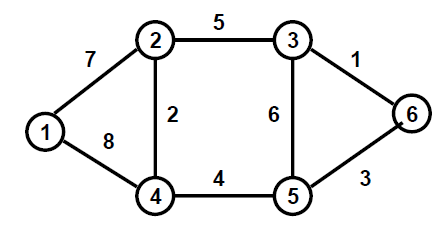
\includegraphics[width=8cm]{ejercicios/grafo no dirigido.png}
    %\caption{Caption}
    %\label{fig:enter-label}
\end{figure}

¿Cuál es árbol generador de peso mínimo? Indica en una lista los arcos que se utilizan en cada paso del algoritmo de Kurskal.

\subsection*{Solución}
El árbol generador de peso mínimo está formado por los arcos en rojo:
\begin{figure}[h!]
    \centering
    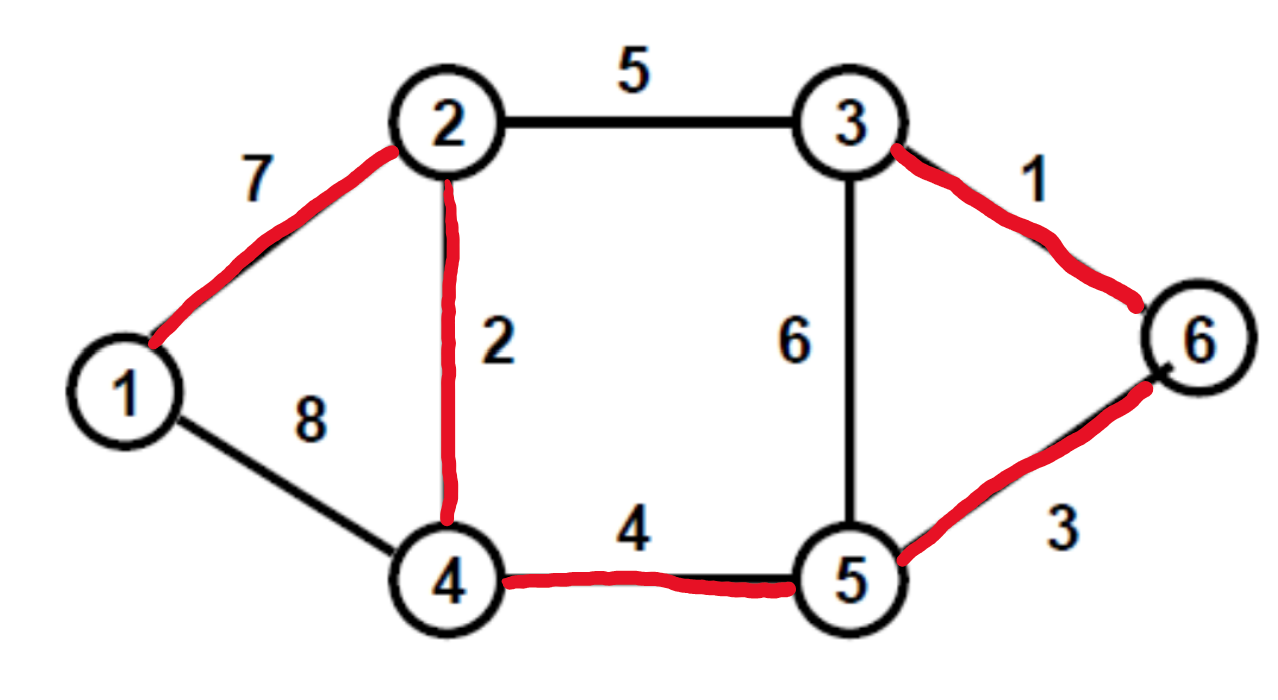
\includegraphics[width=8cm]{ejercicios/grafo_arbol_generador_sol.png}
    %\caption{Caption}
    %\label{fig:enter-label}
\end{figure}

El peso mínimo es 17.
\clearpage
\section{interpretacion artificiales}
En el contexto de la resolución de un problema de programación  lineal, $P$, mediante el método de las dos fases, explicar justificadamente:
\begin{enumerate}
    \item ¿Cuál es la interpretación de la función objetivo correspondiente al problema de la primera fase, $P'$ en relación con el problema $P$?
    \item ¿Qué interpretación tiene el hecho de que la solución óptima de $P'$ tenga función objetivo diferente de cero?
\end{enumerate}
\subsection*{Solución}
En el contexto de la resolución de un problema de programación  lineal, $P$, mediante el método de las dos fases, explicar justificadamente:
\begin{enumerate}
    \item \textbf{¿Cuál es la interpretación de la función objetivo correspondiente al problema de la primera fase, $P'$ en relación con el problema $P$?}

    La función objetivo de $P'$ tiene la forma max. $z' = -\sum_i a_i$ donde $a_i$ es la variable artificial de la restricción $i$, equivalente a min. $-z' = \sum_i a_i$

    Como $a_i$ representa el grado de incumplimiento de la restricción $i$ del problema original, la función objetivo del problema $P'$ representa la suma de los incumplimientos de las restricciones del problema original, $P$.
    
    \item \textbf{¿Qué interpretación tiene el hecho de que la solución óptima de $P'$ tenga función objetivo diferente de cero?}

    Si para la solución óptima de $P'$ existe al menos alguna restricción que no se cumple (existe $a_i>0$), quiere decir que no es posible encontrar una solución de $P'$ que cumpla con todas las restricciones de $P$ que, por lo tanto, es un problema que no tiene solución factible.
    
\end{enumerate}

\clearpage
\section{lemke}
Dado el siguiente problema:

\begin{equation}
\begin{split}
\mbox{min. } z = 10x_1 + 20x_2 + 30x_3\\
s.a.:\\
4x_1 + 2x_2 + 8x_3 \leq 1000\\
1x_2 + 1x_3 = 500\\
x_1,\,\,x_2,\,\,x_3\geq 0\\
\end{split}
\end{equation}

Se pide:
\begin{enumerate}
    \item Explicar si cumple los requisitos para que se pueda aplicar el método de Lemke y, si no es así, obtener un problema equivalente que sí cumpla con dichos requisitos.
    \item Obtener la solución óptima del problema haciendo uso del método de Lemke.
\end{enumerate}
\subsection*{Solución}
Dado el siguiente problema:

\begin{equation}
\begin{split}
\mbox{min. } z = 10x_1 + 20x_2 + 30x_3\\
s.a.:\\
4x_1 + 2x_2 + 8x_3 \leq 1000\\
1x_2 + 1x_3 = 500\\
x_1,\,\,x_2,\,\,x_3\geq 0\\
\end{split}
\end{equation}

Se pide:
\begin{enumerate}
    \item \textbf{Explicar si cumple los requisitos para que se pueda aplicar el método de Lemke y, si no es así, obtener un problema equivalente que sí cumpla con dichos requisitos.}

    Podemos reformular el problema como un problema de maximización en forma estándar:

    \begin{equation}
    \begin{split}
    \mbox{max. } z = -10x_1 - 20x_2 - 30x_3\\
    s.a.:\\
    4x_1 + 2x_2 + 8x_3 + h_1 = 1000\\
    1x_2 + 1x_3 = 500\\
    x_1,\,\,x_2,\,\,x_3,\,\,h_1\geq 0\\
    \end{split}
    \end{equation}

    Para aplicar el método de Lemke necesitamos una solución básica que cumpla con el criterio de optimalidad, cosa que ocurre cuando tenemos un problema de máximos sin restricciones de tipo igual y si todos los coeficientes de las variables de la función objetivo son negativos. Basta con que las variables básicas sean las variables de holgura.

    Para poder eliminar la restricción de igualdad podemos crear dos restricciones, una mayor o igual y otra menor o igual, equivalentes a la original:

    \begin{equation}
    \begin{split}
    \mbox{max. } s = -10x_1 - 20x_2 - 30x_3\\
    s.a.:\\
    4x_1 + 2x_2 + 8x_3 + h_1 = 1000\\
    1x_2 + 1x_3 \leq 500\\
    1x_2 + 1x_3 \geq 500\\
    x_1,\,\,x_2,\,\,x_3,\,\,h_1\geq 0\\
    \end{split}
    \end{equation}

    Y, finalmente, podemos formular el problema en forma estándar, que sí cumple con los requisitos para poder aplicar el método de Lemke.

    \begin{equation}
    \begin{split}
    \mbox{max. } s = -10x_1 - 20x_2 - 30x_3\\
    s.a.:\\
    4x_1 + 2x_2 + 8x_3 + h_1 = 1000\\
    1x_2 + 1x_3 + h_2 = 500\\
    1x_2 + 1x_3 - h_3 = 500\\
    x_1,\,\,x_2,\,\,x_3,\,\,h_1,\,\,h_2,\,\,h_3\geq 0\\
    \end{split}
    \end{equation}

    
    \item \textbf{Obtener la solución óptima del problema haciendo uso del método de Lemke.}
    Podemos resolver el problema equivalente, cuya solución óptima es la misma que la del original.

    \begin{center}
    \begin{tabular}{c|c|cccccc|}
     & $s$ & $x_1$ & $x_2$ & $x_3$ & $h_1$ & $h_2$ & $h_3$\\
     & $0$ & $-10$ & $-20$ & $-30$ & $0$ & $0$ & $0$ \\
    \hline
    $h_1$ & 1000  & $4$ & $2$ & $8$ & $1$ & $0$ & $0$\\
    $h_2$ & 500  & $0$ & $1$ & $1$ & $0$ & $1$ & $0$\\
    $h_3$ & -500  & $0$ & $-1$ & $-1$ & $0$ & $0$ & $1$\\
    \hline
          & $10000$ & $-10$ & $0$ & $-10$ & $0$ & $0$ & $-20$ \\
    \hline
    $h_1$ & 0  & $4$ & $0$ & $6$ & $1$ & $0$ & $2$\\
    $h_2$ & 0  & $0$ & $0$ & $0$ & $0$ & $1$ & $1$\\
    $x_2$ & 500  & $0$ & $1$ & $1$ & $0$ & $0$ & $-1$\\
    \hline
    \end{tabular}
    \end{center}

    En la solución óptima del problema original:
    \begin{itemize}
        \item $z=-s=10000$
        \item $x_2=500$
        \item $x_1=x_3=0$
    \end{itemize}



    
\end{enumerate}
\clearpage
\section{lemke a}
Resolver el siguiente problema mediante el \textbf{método de Lemke}.

\begin{equation}
\begin{split}
\mbox{min. } z = 2x_1 + 3x_2 + x_3\\
s.a.:\\
2x_1 + 2x_2 + 4x_3 \geq 430\\
3x_1 + 4x_2 -  x_3 \leq 960\\
x_1,\,\,x_2,\,\,x_3\geq 0\\
\end{split}
\end{equation}
\subsection*{Solución}
Resolver el siguiente problema mediante el \textbf{método de Lemke}.

\begin{equation}
\begin{split}
\mbox{min. } z = 2x_1 + 3x_2 + x_3\\
s.a.:\\
2x_1 + 2x_2 + 4x_3 \geq 430\\
3x_1 + 4x_2 - x_3 \leq 960\\
x_1,\,\,x_2,\,\,x_3\geq 0\\
\end{split}
\end{equation}

\noindent

\textbf{Solución}
El problema se puede formular como sigue:

\begin{equation}
\begin{split}
\mbox{min. } z = 2x_1 + 3x_2 + x_3\\
s.a.:\\
-2x_1 - 2x_2 - 4x_3 + h_1 = -430\\
3x_1 + 4x_2 - x_3 + h_2 = 960\\
x_1,\,\,x_2,\,\,x_3,\,h_1,\,h_2\geq 0\\
\end{split}
\end{equation}

\begin{center}
\begin{tabular}{c|c|ccccc|}
 & $z$ & $x_1$ & $x_2$ & $x_3$ & $h_1$ & $h_2$\\ 
 & 0 & -2 & -3 & -1 & 0 & 0 \\ 
\hline
$h_1$ & -430  & -2 & -2 & -4 & 1 & 0\\ 
$h_2$ & 960  & 3 & 4 & -1 & 0 & 1\\ 
\hline
 & $215/2$ & $-3/2$ & $-5/2$ & 0 & $-1/4$ & 0 \\ 
\hline
$x_3$ & 215/2  & $1/2$ & $1/2$ & 1 & $-1/4$ & 0\\ 
$h_2$ & 2135/2  & $7/2$ & $9/2$ & 0 & $-1/4$ & 1\\ 
\hline
\end{tabular}
\end{center}

\clearpage
\section{lemke b}
Resolver el siguiente problema mediante el \textbf{método de Lemke}.

\begin{equation}
\begin{split}
\mbox{min. } z = 2x_1 + x_2 + 2x_3\\
s.a.:\\
2x_1 + 2x_2 + 2x_3 \geq 400\\
3x_1 + 4x_2 - x_3 \leq 900\\
x_1,\,\,x_2,\,\,x_3\geq 0\\
\end{split}
\end{equation}
\subsection*{Solución}
Resolver el siguiente problema mediante el \textbf{método de Lemke}.

\begin{equation}
\begin{split}
\mbox{min. } z = 2x_1 + x_2 + 2x_3\\
s.a.:\\
2x_1 + 2x_2 + 2x_3 \geq 400\\
3x_1 + 4x_2 - x_3 \leq 900\\
x_1,\,\,x_2,\,\,x_3\geq 0\\
\end{split}
\end{equation}

\noindent
\textbf{Solución}

El problema se puede formular como sigue:

\begin{equation}
\begin{split}
\mbox{min. } z = 2x_1 + x_2 + 2x_3\\
s.a.:\\
-2x_1 - 2x_2 - 2x_3 +h_1 = -400\\
3x_1 + 4x_2 - x_3 + h_2 =  900\\
x_1,\,\,x_2,\,\,x_3,\,h_1,\,h_2\geq 0\\
\end{split}
\end{equation}

\begin{center}
\begin{tabular}{c|c|ccccc|}
 & $z$ & $x_1$ & $x_2$ & $x_3$ & $h_1$ & $h_2$\\ 
 & 0 & -2 & -1 & -2 & 0 & 0 \\ 
\hline
$h_1$ & -400  & -2 & -2 & -2 & 1 & 0\\ 
$h_2$ & 900  & 3 & 4 & -1 & 0 & 1\\ 
\hline
 & 200 & -1 & 0 & -1 & $-1/2$ & 0 \\ 
\hline
$x_2$ & 200  & 1 & 1 & 1 & $-1/2$ & 0\\ 
$h_2$ & 100  & -1 & 0 & -5 & 2 & 1\\ 
\hline
\end{tabular}
\end{center}


\clearpage
\section{miraflores caminomascorto}
La figura indica el mapa de distancias entre los puntos más importantes del municipio de Miraflores de la Sierra.

Calcula, \textit{\textbf{utilizando alguno de los algoritmos explicados a lo largo del curso}}, el camino más corto (distancias) entre el Parque Jerónimo Sastre y la Casa de la Juventud. Indica, para cada iteración del algoritmo, el resultado final de cada iteración.

\begin{figure}[h!]
    \centering
    \rotatebox{90}{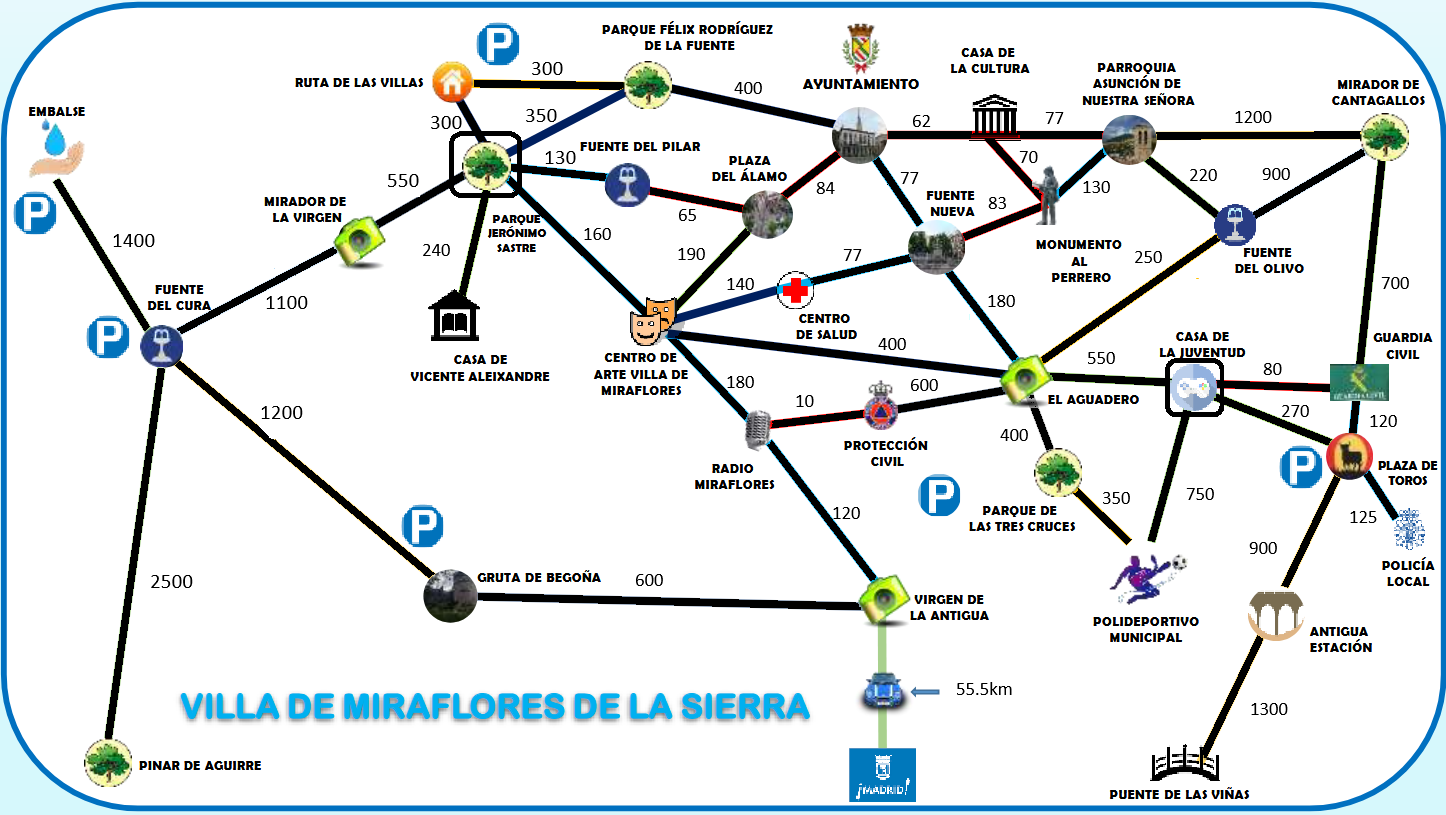
\includegraphics[width=23cm]{ejercicios/miraflores_modificada_final.png} }
\end{figure}


\newpage

\begin{figure}[h!]
    \centering
    \rotatebox{90}{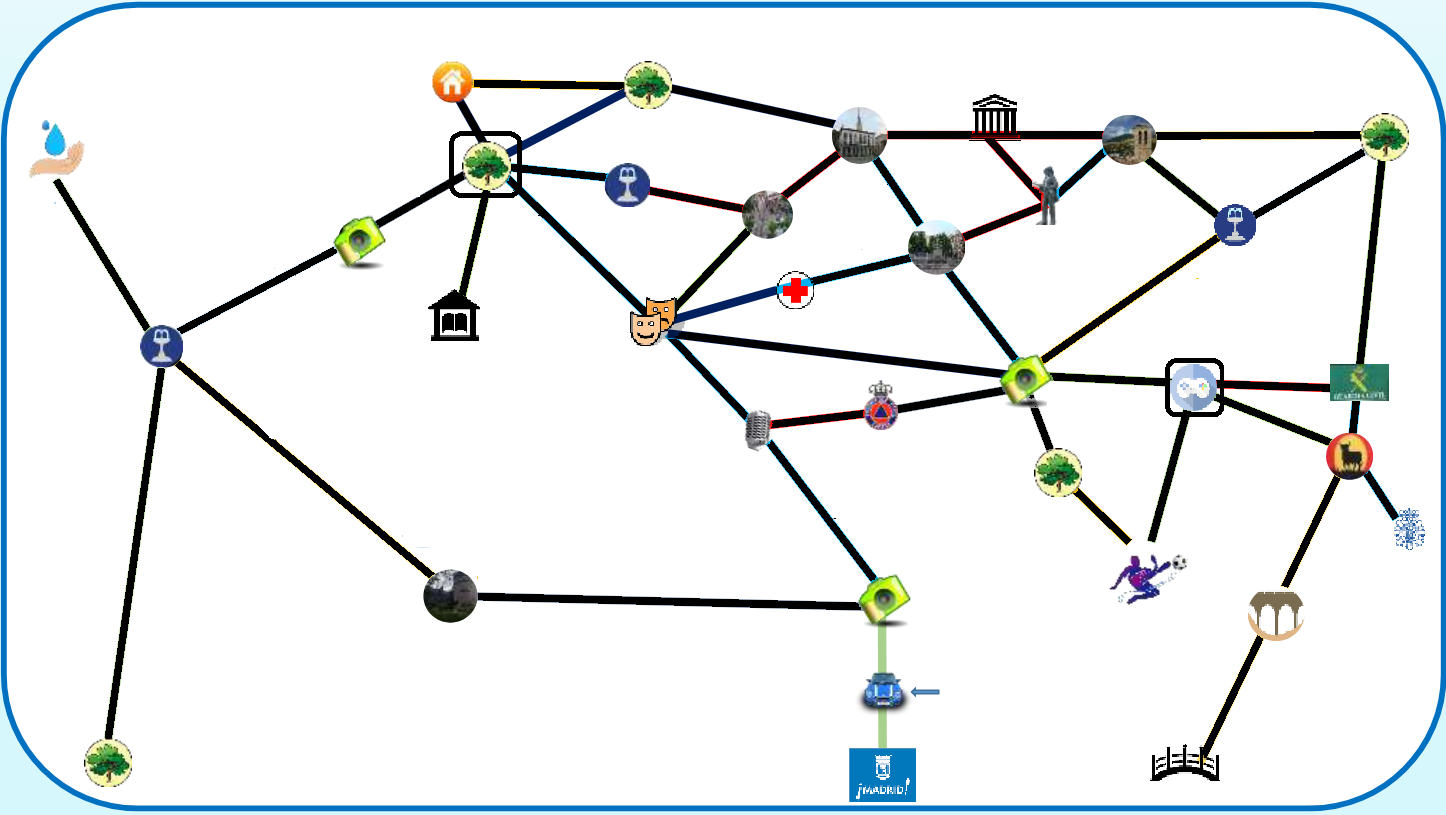
\includegraphics[width=23cm]{ejercicios/miraflores_modificada_limpio_sin_nombres.png} }
\end{figure}

\newpage

\subsection*{Solución}
La figura indica el mapa de distancias entre los puntos más importantes del municipio de Miraflores de la Sierra.

Calcula, \textit{\textbf{utilizando alguno de los algoritmos explicados a lo largo del curso}}, el camino más corto (distancias) entre el Parque Jerónimo Sastre y la Casa de la Juventud. Indica, para cada iteración del algoritmo, el resultado final de cada iteración.

\begin{figure}[h!]
    \centering
    \rotatebox{90}{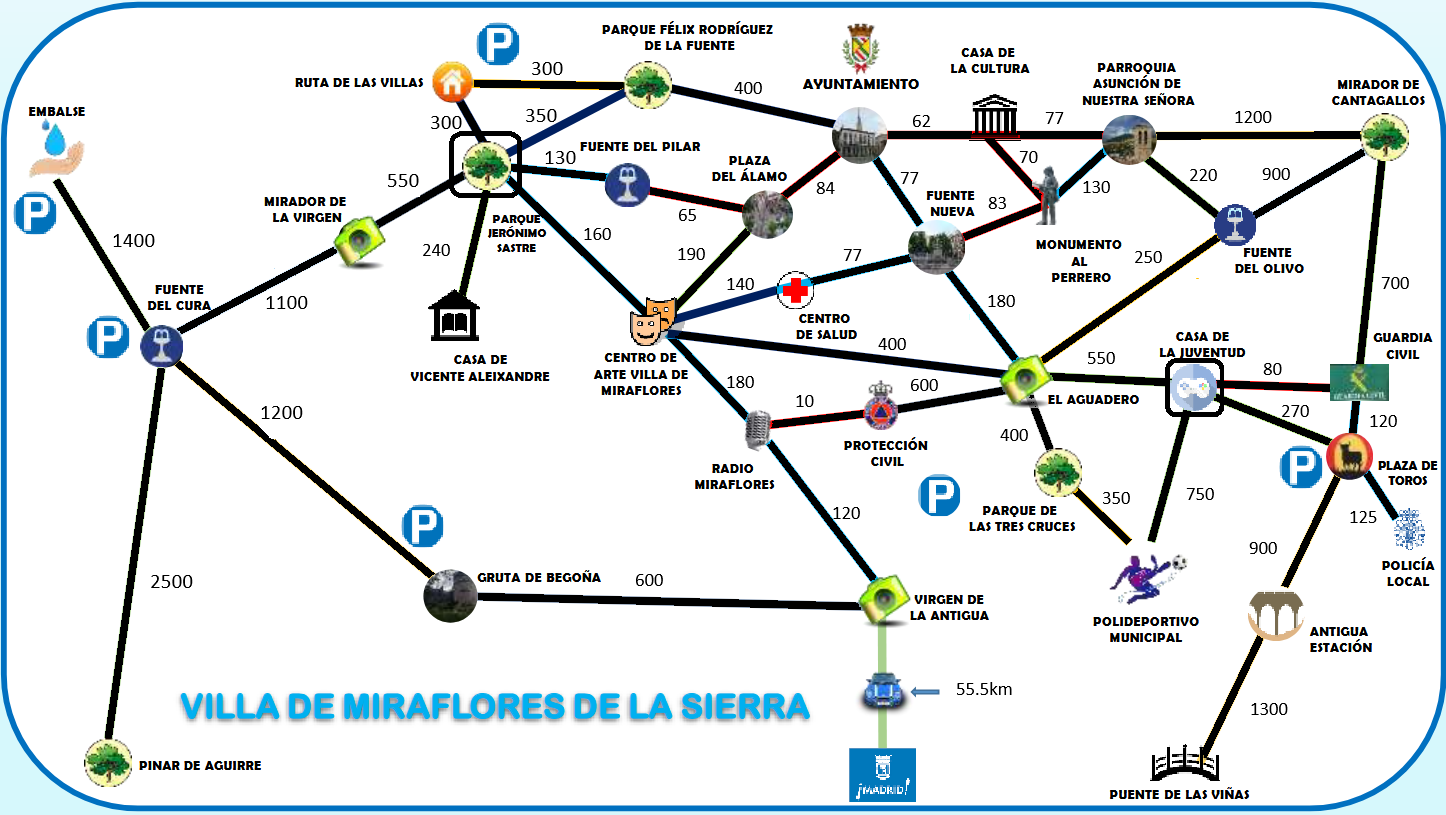
\includegraphics[width=23cm]{ejercicios/miraflores_modificada_final.png} }
\end{figure}

El camino más corto entre el Parque Jerónimo Sastre y la Casa de la Juventud es de 1086 metros pasando por Fuente del Pilar, Plaza del Álamo, Ayuntamiento, Fuente nueva y El aguadero.

\begin{figure}[h!]
    \centering
    \rotatebox{0}{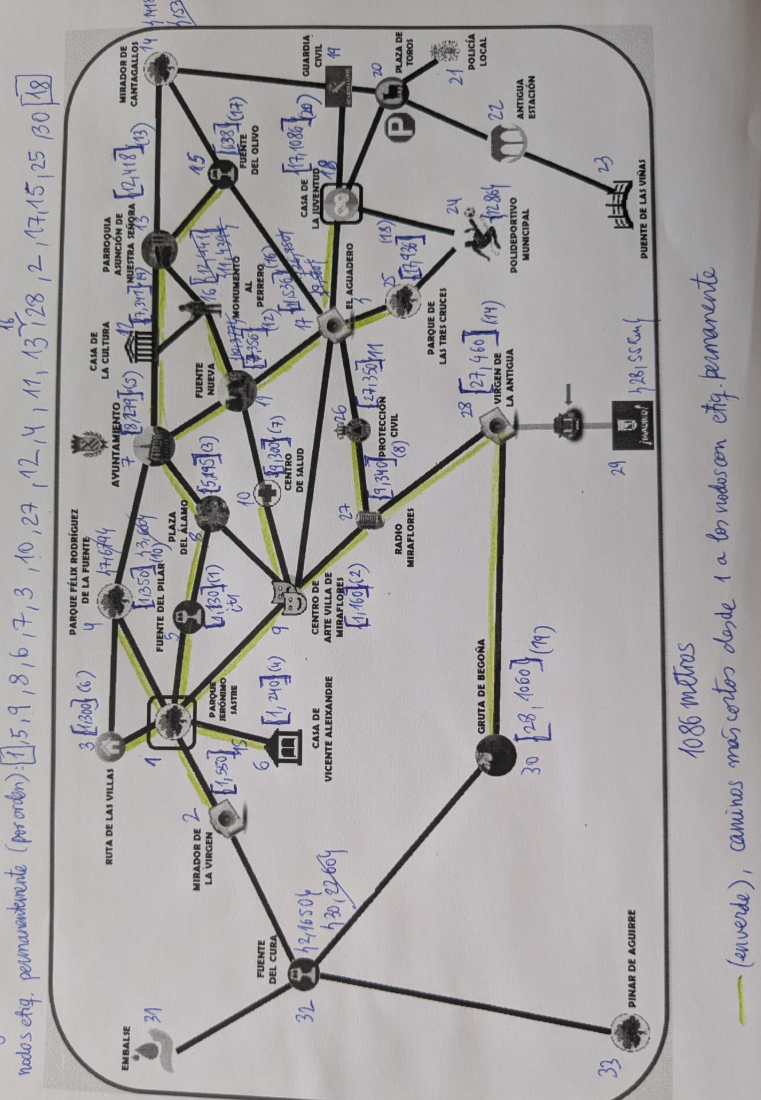
\includegraphics[width=17cm]{ejercicios/miraflores_solución.png} }
\end{figure}
\clearpage
\section{postoptimizacion b teoria}
Dado un problema de programación lineal de la forma 

\begin{align}
    \mbox{max. }&  z =  cx \\
    \mbox{sujeto a: }
    & Ax = b \\
    & x \geq 0
\end{align}

\noindent se conoce la solución óptima, $x^*$, que es básica con base $B$, \textbf{indicar razonadamente} si la siguiente afirmación es cierta:

\noindent "\textit{Si cambia el vector de disponibilidad de los recursos, y toma valor $b'$, la solución óptima será la misma siempre y cuando se cumpla que $B^{-1}b'\geq 0$, es decir, si la solución sigue siendo factible}".
\subsection*{Solución}
Dado un problema de programación lineal de la forma 

\begin{align}
    \mbox{max. } z = & cx \\
    \mbox{sujeto a: }
    & Ax = b \\
    & x \geq 0
\end{align}

\noindent se conoce la solución óptima no degenerada, $x^*$, que es básica con base $B$, \textbf{indicar razonadamente} si la siguiente afirmación es cierta:

\noindent "\textit{Si cambia el vector de disponibilidad de los recursos, y toma valor $b'\neq b$, la solución óptima será la misma siempre y cuando se cumpla que $B^{-1}b'\geq 0$, es decir, si la solución sigue siendo factible}".

\vspace{1cm}

La afirmación es \textbf{incorrecta}. 

Si con el cambio de $b$ a $b'$ se sigue cumpliendo que $B^{-1}b'\geq 0$ y dado que $V^B$ no cambia, la base seguirá siendo óptima. Es decir, la selección de las variables básicas correspondientes a la base $B$ dará lugar a una solución factible y, además, óptima; se trataría de una solución factible y que cumple el criterio de optimalidad.

Sin embargo, sería una base óptima conducente a \textbf{un valor diferente de $u^B$} y de las componentes de $x$ porque los niveles de realización de las variables básicas serán diferentes, porque vienen dados por la expresión $B^{-1}b'$, que son necesariamente diferentes al ser $b'$ diferente y la solución no degenerada. Por lo tanto, la solución óptima sería diferente de la original.






\clearpage
\section{precio sombra no optima}
Una empresa fabrica dos productos químicos, $P_1$ y $P_2$, cuyos márgenes unitarios son, respectivamente, 1 y 4 euros. Semanalmente dispone de 40 toneladas de un producto crítico $C$, que es un cuello de botella. Cada tonelada de $P_1$ consume una tonelada de $C$ y cada tonelada de $P_2$ genera una tonelada de $C$.

Además por normativa, no se pueden producir más de 20 toneladas de $P_2$ y entre los dos productos se deben entregar al menos 10 toneladas.

Un experto el optimización, ha formulado el correspondiente problema de probramación lineal, donde $x_i$ representa la producción en toneladas de $P_i$. 


\begin{equation}
\begin{split}
\mbox{max. } z = x_1 + 4x_2\\
s.a.:\\
x_1 - x_2 \leq 40\\
x_1 + x_2 \geq 10\\
x_2 \leq 20\\
x_1,\,\,x_2\geq 0\\
\end{split}
\end{equation}

Además, ha identificado que el plan de producción actual de la empresa quedaría descrito por la siguiente tabla, correspondiente a una solución básica:

\begin{center}
\begin{tabular}{c|c|ccccc|}
 & $z$ & $x_1$ & $x_2$ & $h_1$ & $h_2$ & $h_3$\\ 
 & $-40$ & $-3$ & $0$ & $0$ & $4$ & $0$ \\ 
\hline
$x_2$ & 10  & $1$ & $1$ & $0$ & $-1$ & $0$\\ 
$h_1$ & 50  & $2$ & $0$ & $1$ & $-1$ & $0$\\ 
$h_3$ & 10  & $-1$ & $0$ & $0$ & $1$ & $1$\\ 
\hline
\end{tabular}
\end{center}



% % \begin{enumerate}
%     A partir de la información de la tabla, justificar por qué relajar el compromiso comercial en una unidad, es decir, reducir $b_2$ en una unidad, daría lugar a una disminución de la función objetivo.
%     % \item Explicar por qué relajar el compromiso comercial (lo cual implica aumentar el tamaño de la región de factibilidad) conduce a una solución con peor función objetivo.
% % \end{enumerate}

\begin{enumerate}
\item A partir de la información de la tabla, justificar que disminuir el compromiso comercial, $b_2$, en una unidad daría lugar a una disminución de la función objetivo.

\item Explicar por qué relajar el compromiso comercial (lo cual implica aumentar el tamaño de la región de factibilidad) conduce a una solución con peor función objetivo.
\end{enumerate}
\subsection*{Solución}
Una empresa fabrica dos productos químicos, $P_1$ y $P_2$, cuyos márgenes unitarios son, respectivamente, 1 y 4 euros. Semanalmente dispone de 40 toneladas de un producto crítico $C$, que es un cuello de botella. Cada tonelada de $P_1$ consume una tonelada de $C$ y cada tonelada de $P_2$ genera una tonelada de $C$.

Además por normativa, no se pueden producir más de 20 toneladas de $P_2$ y entre los dos productos se deben entregar al menos 10 toneladas.

Un experto el optimización, ha formulado el correspondiente problema de probramación lineal, donde $x_i$ representa la producción en toneladas de $P_i$. 


\begin{equation}
\begin{split}
\mbox{max. } z = x_1 + 4x_2\\
s.a.:\\
x_1 - x_2 \leq 40\\
x_1 + x_2 \geq 10\\
x_2 \leq 20\\
x_1,\,\,x_2\geq 0\\
\end{split}
\end{equation}

Además, ha identificado que el plan de producción actual de la empresa quedaría descrito por la siguiente tabla, correspondiente a una solución básica:

\begin{center}
\begin{tabular}{c|c|ccccc|}
 & $z$ & $x_1$ & $x_2$ & $h_1$ & $h_2$ & $h_3$\\ 
 & $-40$ & $-3$ & $0$ & $0$ & $4$ & $0$ \\ 
\hline
$x_2$ & 10  & $1$ & $1$ & $0$ & $-1$ & $0$\\ 
$h_1$ & 50  & $2$ & $0$ & $1$ & $-1$ & $0$\\ 
$h_3$ & 10  & $-1$ & $0$ & $0$ & $1$ & $1$\\ 
\hline
\end{tabular}
\end{center}



\begin{enumerate}
    \item \textbf{A partir de la información de la tabla, justificar que disminuir el compromiso comercial, $b_2$ en una unidad daría lugar a una disminución de la función objetivo.}
    

    El incremento (disminución) de $z$ cuando $b_2$ aumenta (disminuye) en un unidad viene dado por el precio sombra de la segunda restricción, $\pi^B_2 = V^B_{h_2}=4$ (restricción de tipo menor o igual).

    En efecto si $b_2=9$, $z$ disminuye en 4 unidades (4000 euros).


    \item \textbf{Explicar por qué relajar el compromiso comercial (lo cual implica aumentar el tamaño de la región de factibilidad) conduce a una solución con peor función objetivo.}

    La explicación de esta aparente paradoja viene dada por el hecho de que la solución no es óptima. La base a la que se refiere la tabla tiene como variables básicas: $x_2$, $h_1$ y $h_3$, es decir corresponden a la intersección de la restricción 2 con el eje de $Y$, como se aprecia en la siguiente figura.

\begin{tikzpicture}
    \begin{axis}[
        axis lines = middle,
        xlabel = {$x_1$},
        ylabel = {$x_2$},
        xmin = 0, xmax = 70,
        ymin = 0, ymax = 40,
        width=14cm, height=10cm,
        legend pos = north west,
        grid = major,
    ]
    % Restriction 1: x1 - x2 <= 40
    \addplot[name path=A, domain=0:70, thick, blue] {x - 40};
    \addlegendentry{$x_1 - x_2 \leq 40$}

    % Restriction 2: x1 + x2 >= 10
    \addplot[name path=B, domain=0:70, thick, red] {10 - x};
    \addlegendentry{$x_1 + x_2 \geq 10$}

    % Restriction 3: x2 <= 20
    \addplot[name path=C, domain=0:70, thick, green!70!black] {20};
    \addlegendentry{$x_2 \leq 20$}

    % Region Factible (shading)
    \addplot [
        thick,
        color=yellow,
        fill=yellow,
        fill opacity=0.3
    ]
    coordinates {
        (10,0) (0,10) (0,20) (60, 20) (40,0)
    };

    % Objective function line (longer)
    \addplot[dashed, thick, black, domain=-10:80] {0.25*x + 8};
    \addlegendentry{F. objetivo $z = 1x_1 + 4x_2$}

        % Adding the label for the point
    \node[circle, draw=black, minimum size=6pt, inner sep=0pt] at (axis cs:0, 10) {};
    \node at (axis cs:8, 10) [anchor=south] {Solución básica};
    
    \end{axis}
\end{tikzpicture}

    Relajar el compromiso comercial significa desplazar la restricción 2 hacia la izquierda, con lo que la solución básica, intersección de esta restricción 2 con el eje $Y$ haría que disminuyera $z$.

    La interpretación es la siguiente. En esta base:
    \begin{itemize}
        \item $x_1$ es variable no básica, con lo que se decide no producir $P_1$
        \item $h_2$ es variable no básica, con lo se está decidiendo cumplir el compromiso comercial por el mínimo acordado.
    \end{itemize}

    Si queremos producir solo lo que viene dado por el compromiso comercial ($h_2=0$) y solo se produce $P_2$ ($x_1=0$) el resultado es que se produce solo $P_2$ y en menor cantidad, con lo que la función objetivo disminuye.


    Este comportamiento no se observaría si estuviéramos en la solución óptima.



\end{enumerate}
\clearpage
\section{precio sombra sol opt}
En un problema de programación lineal de maximización, dada una restricción de tipo menor o igual, ¿qué se puede afirmar sobre el signo del precio sombra de dicha restricción correspondiente una solución básica y óptima del problema? \textbf{Justificar} la respuesta.
\subsection*{Solución}
En un problema de programación lineal de maximización, dada una restricción de tipo menor o igual, ¿qué se puede afirmar sobre el signo del precio sombra de dicha restricción correspondiente una solución básica y óptima del problema?
\vspace{1cm}

\noindent
\textbf{Solución}

\vspace{0.5cm}

Cualquier solución básica óptima cumple que $V^B \leq 0$. Por otro lado, el precio sombra de una restricción menor o igual es igual al criterio del simplex correspondiente a la variable de holgura de dicha restricción cambiado de signo, es decir, $\pi^B_i = -V^B_{h_i}$. Por lo tanto, $\pi^B_i \geq 0$, el precio sombra es no negativo en la solución óptima.

\clearpage
\section{quimica a}
Una empresa química fabrica tres tipos de productos químicos, P1, P2 y P3, cuyos beneficios unitarios son, respectivamente, \textbf{2, 2 y 4} unidades monetarias (u.m.) 

Para su producción, se consumen dos materias primas. En particular, se consumen \textbf{1} tonelada de materia prima M1 y \textbf{2} de materia prima M2 por cada tonelada de P1, \textbf{2} de M1 y \textbf{1} de M2 por cada tonelada de P2 y \textbf{3} de M1 y \textbf{4} de M2 por cada tonelada de P3.

Cada mes, se dispone de \textbf{400} y \textbf{260} toneladas de materias primas M1 y M2, respectivamente. 

Por cada tonelada de P2 se generan \textbf{2} toneladas de un subproducto peligroso. Por cada tonelada de P1 se consume \textbf{1} tonelada del mismo subproducto. A su vez, por cada tonelada de de P3 se consume \textbf{1} tonelada de dicho subproducto. La empresa es autosuficiente con este subproducto y no dispone de ninguna cantidad adicional comprada, de forma que todo lo que necesita para P1 y P3 se genera mediante la producción de P2.


Para obtener el programa de producción de máximo beneficio se dispone del siguiente modelo de programación lineal, donde $x_1$, $x_2$ y $x_3$ representan las toneladas mensuales producidas de P1, P2 y P3, respectivamente.
 
\begin{equation}
\begin{split}
\mbox{max. } z = 2x_1 + 2x_2 + 4x_3\\
s.a.:\\
1x_1 + 2x_2 + 3x_3 \leq 400\\
2x_1 + 1x_2 + 4x_3 \leq 260\\
1x_1 - 2x_2 + 1x_3 = 0\\
x_1,\,\,x_2,\,\,x_3\geq 0\\
\end{split}
\end{equation}

Se conoce la tabla correspondiente a la solución óptima.

\begin{center}
\begin{tabular}{c|c|ccccc|}
 & $z$ & $x_1$ & $x_2$ & $x_3$ & $h_1$ & $h_2$\\ 
      & -312 & 0 & 0 & $-2/5$ & 0 & $-6/5$ \\ 
\hline
$h_1$ & 192  & 0 & 0 & 2/5 & 1 & $-4/5$\\ 
$x_2$ & 52  & 0 & 1 & $2/5$ & 0 & 1/5\\ 
$x_1$ & 104  & 1 & 0 & 9/5 & 0 & 2/5\\ 
\hline
\end{tabular}
\end{center}

\begin{enumerate}
    \item Interpretar la información que proporciona la tabla correspondiente a la solución óptima.

    \item Dentro de qué rango de valores puede variar el beneficio del producto P1 sin que cambie la gama de productos que resulta más beneficioso producir.

    \item Ha surgido la necesidad de producir 1 tonelada de producto P3, ¿cuál sería el nuevo valor del beneficio y el nuevo plan de la producción?
    
    \item ¿Qué impacto tendría sobre el beneficio la posibilidad de comprar y disponer de una tonelada de subproducto (diferente de las que se generan con la producción de P2)? Si la empresa dispone de ese producto adicional, dada la naturaleza peligrosa del mismo, debería consumirlo obligatoriamente.
    
\end{enumerate}







\subsection*{Solución}
Una empresa química fabrica tres tipos de productos químicos, P1, P2 y P3, cuyos beneficios unitarios son, respectivamente, \textbf{2, 2 y 4} unidades monetarias (u.m.) 

Para su producción, se consumen dos materias primas. En particular, se consumen \textbf{1} tonelada de materia prima M1 y \textbf{2} de materia prima M2 por cada tonelada de P1, \textbf{2} de M1 y \textbf{1} de M2 por cada tonelada de P2 y \textbf{3} de M1 y \textbf{4} de M2 por cada tonelada de P3.

Cada mes, se dispone de \textbf{400} y \textbf{260} toneladas de materias primas P1 y P2, respectivamente. 

Por cada tonelada de P2 se generan \textbf{2} toneladas de un subproducto peligroso. Por cada tonelada de P1 se genera \textbf{1} tonelada del mismo subproducto. A su vez, por cada tonelada de de P3 se consume \textbf{1} toneladas de dicho subproducto. La empresa es autosuficiente con este subproducto y no dispone de ninguna cantidad adicional comprada, de forma que todo lo que necesita para P2 se genera mediante la producción de P1 y P3.


Para obtener el programa de producción de máximo beneficio se dispone del siguiente modelo de programación lineal, donde $x_1$, $x_2$ y $x_3$ representan las toneladas mensuales producidas de P1, P2 y P3, respectivamente.
 
\begin{equation}
\begin{split}
\mbox{max. } z = 2x_1 + 2x_2 + 4x_3\\
s.a.:\\
1x_1 + 2x_2 + 3x_3 \leq 400\\
2x_1 + 1x_2 + 4x_3 \leq 260\\
1x_1 - 2x_2 + 1x_3 = 0\\
x_1,\,\,x_2,\,\,x_3\geq 0\\
\end{split}
\end{equation}

Se conoce la tabla correspondiente a la solución óptima.

\begin{center}
\begin{tabular}{c|c|ccccc|}
 & $z$ & $x_1$ & $x_2$ & $x_3$ & $h_1$ & $h_2$\\ 
Phase 2 & -312 & 0 & 0 & $\frac{-2}{5}$ & 0 & $\frac{-6}{5}$ \\ 
\hline
$h_1$ & 192  & 0 & 0 & $\frac{2}{5}$ & 1 & $\frac{-4}{5}$\\ 
$x_2$ & 52  & 0 & 1 & $\frac{2}{5}$ & 0 & $\frac{1}{5}$\\ 
$x_1$ & 104  & 1 & 0 & $\frac{9}{5}$ & 0 & $\frac{2}{5}$\\ 
\hline
\end{tabular}
\end{center}

\begin{enumerate}
    \item Interpretar la información que proporciona la tabla correspondiente a la solución óptima.

    El plan de producción que ofrece el mayor beneficio:
    \begin{itemize}
        \item Proporciona un beneficio total de 312 u.m.
        \item Se producen 104 toneladas de P1.
        \item Se producen 52 toneladas de P2.
        \item No se emplean 192 de las 400 toneladas disponibles de M1.
        \item Se emplean por completo las 250 toneladas disponibles de M2.
    \end{itemize}

    \item Dentro de qué rango de valores puede variar el beneficio del producto P1 sin que cambie la gama de productos que resulta más beneficioso producir.

    Es necesario realizar el análisis de sensibilidad de $c_1$.

    Para que la gama siga siendo la misma, la base óptima debe seguir siéndolo y eso pasa porque $V^B \leq 0$

    \begin{equation}
    \begin{split}
    V^B = c-c^BB^{-1}A = c-c^Bp^B = \\
    = \begin{pmatrix}
    c_1 & 2 & 4 & 0 & 0\\
    \end{pmatrix}
     - \begin{pmatrix}
    0 & 2 & c_1\\
    \end{pmatrix}
    \begin{pmatrix}
    1 & \frac{-4}{5} & \frac{3}{5}\\
    0 & \frac{1}{5} & \frac{-2}{5}\\
    0 & \frac{2}{5} & \frac{1}{5}\\
    \end{pmatrix}
    \begin{pmatrix}
    1 & 2 & 3 & 1 & 0\\
    2 & 1 & 4 & 0 & 1\\
    1 & -2 & 1 & 0 & 0\\
    \end{pmatrix}
     = \\
     \begin{pmatrix}
    c_1 & 2 & 4 & 0 & 0\\
    \end{pmatrix}
     - \begin{pmatrix}
    0 & 2 & c_1\\
    \end{pmatrix}
    \begin{pmatrix}
    0 & 0 & 2/5 & 1 & -4/5\\
    0 & 1 & 2/5 & 0 & 1/5\\
    1 & 0 & 9/5 & 0 & 2/5\\
    \end{pmatrix} 
    = \\
     \begin{pmatrix}
    c_1 & 2 & 4 & 0 & 0\\
    \end{pmatrix}
    -
     \begin{pmatrix}
     c_1 &  2 & \frac{4+9c_1}{5} & 0 & \frac{2+2c_1}{5}  \\
    \end{pmatrix} = \\
     \begin{pmatrix}
     0 &  0 & \frac{16-9c_1}{5} & 0 & -\frac{2+2c_1}{5} \\
    \end{pmatrix}
     \leq 0
    \end{split}
    \end{equation}

    Por lo tanto, se debe cumplir $\frac{16-9c_1}{5} \leq 0$ y $-\frac{2+2c_1}{5} \leq 0$, es decir, $\frac{16}{9} \leq c_1$ y $-1 \leq c_1$.

    Mientras el margen del producto P1 sea igual o superior a $\frac{16}{9} = 1.78$ (y lo es), la gama de productos es la que se indica en el apartado anterior.



    \item Ha surgido la necesidad de producir 1 tonelada de producto P3, ¿qué impacto tendría sobre el beneficio y sobre el resto de la producción?

    Producir una tonelada de P3 implicaría que $x_3 = 1$. En la solución óptima $x_3$ es una variable no básica y, por lo tanto, su valor es nulo. El impacto de aumentar una unidad $x_3$ queda reflejado en:

    \begin{itemize}
        \item El criterio del simplex, $V^B_3 = -2/5$. Por lo que al producir una tonelada adicional, el beneficio disminuiría en 2/5 u.m.
        \item Las tasas de sustitución dan cuenta de la modificación de los valores de las variables básicas. En este caso:
        \begin{itemize}
            \item $p^B_{13} = 2/5$, $h_1$ disminuiría una 2/5, es decir, se haría uso de 400 kg más de M1.
            \item $p^B_{23} = 2/5$, $x_2$ disminuiría en 2/5, es decir, se producirían 400 kg menos de producto P2.
            \item $p^B_{33} = 9/5$, $x_1$ disminuiría en 9/5, es decir, se producirían 1.8 toneladas menos de producto $P_1$.
        \end{itemize}
    \end{itemize}

     
    
    \item ¿Qué impacto tendría sobre el beneficio la posibilidad de comprar y disponer de una tonelada de subproducto (diferente de las que se generan con la producción de P1 y P3)? Si la empresa dispone de ese producto adicional, dada la naturaleza peligrosa del mismo, debería consumirlo obligatoriamente.

    El hecho de que se disponga de una unidad más de subproducto sería equivalente a que la tercer restricción tuviera la forma:
    
    $$1x_1 - 2x_2 + 1x_3 = 1$$

    Es decir, el términos $b_3$ aumentaría una unidad. El precio sombra de la restricción 3 es igual al incremento de la función objetivo cuando se aumenta una unidad la disponibilidad del recurso correspondiente a esa restricción (parta derecha de la ecuación). Es decir, $\pi^B_3 = \Delta z|_{\Delta h_3 = 1}$

    Para calcular el precio sombra es necesario disponer de la inversa de la base:

    \begin{equation}
    \begin{split}
    B^{-1} =\begin{pmatrix}
    1 & -4/5 & 3/5\\
    0 & 1/5 & -2/5\\
    0 & 2/5 & 1/5\\
    \end{pmatrix}
    \end{split}
    \end{equation}
    
    El precio sombra se calcula como:

    \begin{equation}
    \begin{split}
    \pi^B = c^BB^{-1} = \begin{pmatrix}
    0 & 2 & 2\\
    \end{pmatrix}
    \begin{pmatrix}
    1 & -4/5 & 3/5\\
    0 & 1/5 & -2/5\\
    0 & 2/5 & 1/5\\
    \end{pmatrix}
     = \begin{pmatrix}
    0 & 6/5 & -2/5\\
    \end{pmatrix}
    \end{split}
    \end{equation}
    
    El precio sombra de la restricción 3 es -2/5, lo cual quiere decir que si se dispusiera de 1 tonelada del subproducto peligroso, la función objetivo disminuiría en 2/5 u.m.
    
\end{enumerate}







\clearpage
\section{quimica b}
Una empresa química fabrica tres tipos de productos químicos, P1, P2 y P3, cuyos beneficios unitarios son, respectivamente, \textbf{1, 2 y 4} unidades monetarias (u.m.) 

Para su producción, se consumen dos materias primas. En particular, se consumen \textbf{1} tonelada de materia prima M1 y \textbf{2} de materia prima M2 por cada tonelada de P1, \textbf{2} de M1 y \textbf{1} de M2 por cada tonelada de P2 y \textbf{2} de M1 y \textbf{4} de M2 por cada tonelada de P3.

Cada mes, se dispone de \textbf{200} y \textbf{500} toneladas de materias primas P1 y P2, respectivamente. 

Por cada tonelada de P2 se generan \textbf{2} toneladas de un subproducto peligroso. Por cada tonelada de P1 se genera \textbf{1} tonelada del mismo subproducto. A su vez, por cada tonelada de de P3 se consume \textbf{1} toneladas de dicho subproducto. La empresa es autosuficiente con este subproducto y no dispone de ninguna cantidad adicional comprada, de forma que todo lo que necesita para P2 se genera mediante la producción de P1 y P3.

Para obtener el programa de producción de máximo beneficio se dispone del siguiente modelo de programación lineal, donde $x_1$, $x_2$ y $x_3$ representan las toneladas mensuales producidas de P1, P2 y P3, respectivamente.
 
\begin{equation}
\begin{split}
\mbox{max. } z = x_1 + 2x_2 + 4x_3\\
s.a.:\\
 x_1 + 2x_2 + 2x_3 \leq 200\\
2x_1 +  x_2 + 4x_3 \leq 500\\
 x_1 - 2x_2 +  x_3 = 0\\
x_1,\,\,x_2,\,\,x_3\geq 0\\
\end{split}
\end{equation}

Se conoce la tabla correspondiente a la solución óptima.

\begin{center}
\begin{tabular}{c|c|ccccc|}
 & $z$ & $x_1$ & $x_2$ & $x_3$ & $h_1$ & $h_2$\\ 
      & $-1000/3$ & $-4/3$ & 0 & 0 & $-5/3$ & 0 \\ 
\hline
$x_2$ & 100/3  & $-1/6$ & 1 & 0 & $1/6$ & 0\\ 
$h_2$ & 200  & $-1/2$ & 0 & 0 & $-3/2$ & 1\\ 
$x_3$ & 200/3  & $2/3$ & 0 & 1 & $1/3$ & 0\\ 
\hline
\end{tabular}
\end{center}





\begin{enumerate}
    \item Interpretar la información que proporciona la tabla correspondiente a la solución óptima.

    \item Dentro de qué rango de valores puede variar el beneficio del producto P2 sin que cambie la gama de productos que resulta más beneficioso producir.
    
    \item Ha surgido la necesidad de producir 1 tonelada de producto P1, ¿qué impacto tendría sobre el beneficio y sobre el resto de la producción?
        
    \item ¿Qué impacto tendría sobre el beneficio la posibilidad de comprar y disponer de una tonelada de subproducto (diferente de las que se generan con la producción de P1 y P3)? Si la empresa dispone de ese producto adicional, dada la naturaleza peligrosa del mismo, debería consumirlo obligatoriamente.

    
\end{enumerate}







\subsection*{Solución}
Una empresa química fabrica tres tipos de productos químicos, P1, P2 y P3, cuyos beneficios unitarios son, respectivamente, \textbf{1, 2 y 4} unidades monetarias (u.m.) 

Para su producción, se consumen dos materias primas. En particular, se consumen \textbf{1} tonelada de materia prima M1 y \textbf{2} de materia prima M2 por cada tonelada de P1, \textbf{2} de M1 y \textbf{1} de M2 por cada tonelada de P2 y \textbf{2} de M1 y \textbf{4} de M2 por cada tonelada de P3.

Cada mes, se dispone de \textbf{200} y \textbf{500} toneladas de materias primas P1 y P2, respectivamente. 

Por cada tonelada de P2 se generan \textbf{2} toneladas de un subproducto peligroso. Por cada tonelada de P1 se genera \textbf{1} tonelada del mismo subproducto. A su vez, por cada tonelada de de P3 se consume \textbf{1} toneladas de dicho subproducto. La empresa es autosuficiente con este subproducto y no dispone de ninguna cantidad adicional comprada, de forma que todo lo que necesita para P2 se genera mediante la producción de P1 y P3.

Para obtener el programa de producción de máximo beneficio se dispone del siguiente modelo de programación lineal, donde $x_1$, $x_2$ y $x_3$ representan las toneladas mensuales producidas de P1, P2 y P3, respectivamente.
 
\begin{equation}
\begin{split}
\mbox{max. } z = x_1 + 2x_2 + 4x_3\\
s.a.:\\
 x_1 + 2x_2 + 2x_3 \leq 200\\
2x_1 +  x_2 + 4x_3 \leq 500\\
 x_1 - 2x_2 +  x_3 = 0\\
x_1,\,\,x_2,\,\,x_3\geq 0\\
\end{split}
\end{equation}

Se conoce la tabla correspondiente a la solución óptima.

\begin{center}
\begin{tabular}{c|c|ccccc|}
 & $z$ & $x_1$ & $x_2$ & $x_3$ & $h_1$ & $h_2$\\ 
      & $-1000/3$ & $-4/3$ & 0 & 0 & $-5/3$ & 0 \\ 
\hline
$x_2$ & 100/3  & $-1/6$ & 1 & 0 & $1/6$ & 0\\ 
$h_2$ & 200  & $-1/2$ & 0 & 0 & $-3/2$ & 1\\ 
$x_3$ & 200/3  & $2/3$ & 0 & 1 & $1/3$ & 0\\ 
\hline
\end{tabular}
\end{center}





\begin{enumerate}
    \item Interpretar la información que proporciona la tabla correspondiente a la solución óptima.

    El plan de producción que ofrece el mayor beneficio:
    \begin{itemize}
        \item Proporciona un beneficio total de 333.33 u.m.
        \item No se produce P1
        \item Se producen 33.33 toneladas de P2.
        \item Se producen 66.67 toneladas de P3.
        \item Se emplean por completo las 200 toneladas disponibles de M1.
        \item No se emplean 200 de las 500 toneladas disponibles de M2.
        
    \end{itemize}

    \item Dentro de qué rango de valores puede variar el beneficio del producto P2 sin que cambie la gama de productos que resulta más beneficioso producir.

    Es necesario realizar el análisis de sensibilidad de $c_2$.

    Para que la gama siga siendo la misma, la base óptima debe seguir siéndolo y eso pasa porque $V^B \leq 0$

    \begin{equation}
    \begin{split}
    V^B = c-c^BB^{-1}A = c-c^Bp^B =\\
    = \begin{pmatrix}
    1 & c_2 & 4 & 0 & 0\\
    \end{pmatrix}
     - \begin{pmatrix}
    c_2 & 0 & 4\\
    \end{pmatrix}
    \begin{pmatrix}
    -1/6 & 1 & 0 & 1/6 & 0\\
    -1/2 & 0 & 0 & -3/2 & 1\\
    2/3 & 0 & 1 & 1/3 & 0\\
    \end{pmatrix}
     = \\
     =\begin{pmatrix}
    1 & c_2 & 4 & 0 & 0\\
    \end{pmatrix} - 
     \begin{pmatrix}
    \frac{-c_2+16}{6}  &  c_2  & 4 & \frac{c_2+8}{6}  & 0 \\
    \end{pmatrix}=   \\  
     =\begin{pmatrix}
     \frac{-10+c_2}{6}& 0 & 0 & -\frac{c_2+8}{6} & 0\\
    \end{pmatrix} \leq 0
    \end{split}
    \end{equation}
        
    
    Por lo tanto, se debe cumplir $\frac{-10+c_2}{6} \leq 0$ y $-\frac{c_2+8}{6} \leq 0$, es decir, $c_2 \leq 10$ y $c_2 \geq -8$.

    Mientras el margen del producto P1 sea igual o superior a $-8$ (no de pérdidas superiores a 8 u.m.) y no sea mayor 10, la gama de productos es la que se indica en el apartado anterior.



    \item Ha surgido la necesidad de producir 1 tonelada de producto P1, ¿qué impacto tendría sobre el beneficio y sobre el resto de la producción?

    Producir una tonelada de P3 implicaría que $x_1 = 1$. En la solución óptima $x_1$ es una variable no básica y, por lo tanto, su valor es nulo. El impacto de aumentar una unidad $x_1$ queda reflejado en:

    \begin{itemize}
        \item El criterio del simplex, $V^B_3 = -4/3$. Por lo que al producir una tonelada adicional, el beneficio disminuiría en 4/3 u.m.
        \item Las tasas de sustitución dan cuenta de la modificación de los valores de las variables básicas. En este caso:
        \begin{itemize}
            \item $p^B_{11} = -1/6$, $x_2$ aumentaría 1/6, es decir, se producirían 166.67 kg más de $P_2$.
            \item $p^B_{21} = -1/2$, $h_2$ aumentaría en 1/2, es decir, se haría uso de 500 kg menos de $M_2$.
            \item $p^B_{31} = 2/3$, $x_3$ disminuiría en 2/3, es decir, se producirían 666.67 kg menos de producto $P_3$.
        \end{itemize}
    \end{itemize}

     
    
    \item ¿Qué impacto tendría sobre el beneficio la posibilidad de comprar y disponer de una tonelada de subproducto (diferente de las que se generan con la producción de P1 y P3)? Si la empresa dispone de ese producto adicional, dada la naturaleza peligrosa del mismo, debería consumirlo obligatoriamente.

    El hecho de que se disponga de una unidad más de subproducto sería equivalente a que la tercer restricción tuviera la forma:
    
    $$1x_1 - 2x_2 + 1x_3 = 1$$

    Es decir, el términos $b_3$ aumentaría una unidad. El precio sombra de la restricción 3 es igual al incremento de la función objetivo cuando se aumenta una unidad la disponibilidad del recurso correspondiente a esa restricción (parta derecha de la ecuación). Es decir, $\pi^B_3 = \Delta z|_{\Delta h_3 = 1}$

    Para calcular el precio sombra es necesario disponer de la inversa de la base:

    \begin{equation}
    \begin{split}
    B^{-1} =\begin{pmatrix}
    1/6 & 0 & -1/3\\
    -3/2 & 1 & -1\\
    1/3 & 0 & 1/3\\
    \end{pmatrix}
    \end{split}
    \end{equation}
    
    El precio sombra se calcula como:

    \begin{equation}
    \begin{split}
    \pi^B = c^BB^{-1} = \begin{pmatrix}
    2 & 0 & 4\\
    \end{pmatrix}
    \begin{pmatrix}
    1/6 & 0 & -1/3\\
    -3/2 & 1 & -1\\
    1/3 & 0 & 1/3\\
    \end{pmatrix}
     = \begin{pmatrix}
    5/3 & 0 & 2/3\\
    \end{pmatrix}
    \end{split}
    \end{equation}
    
    El precio sombra de la restricción 3 es 2/3, lo cual quiere decir que si se dispusiera de 1 tonelada del subproducto peligroso, la función objetivo aumentaría en 2/3 u.m.
    
\end{enumerate}







\clearpage
\section{red gas kurskal}


Una importante corporación energética global está planificando la interconexión de diez núcleos urbanos importantes (C1 a C10) para su nueva red de distribución de gas. El objetivo principal es construir una red de tuberías que garantice que todas las ciudades estén conectadas y puedan recibir suministro de gas, pero minimizando estrictamente el coste total de la infraestructura. Se han realizado estudios detallados para determinar el coste exacto de instalar tuberías entre cada par de ciudades conectables, y estos costes son todos diferentes entre sí.

El grafo no dirigido asociado se ha representado con la siguiente \textbf{matriz de adyacencia}. La matriz presenta las diez ciudades (nodos) y los 18 posibles tramos de tubería entre ellas, con sus costes asociados. Un valor de 0 indica que no hay conexión directa posible o que se refiere a la misma ciudad.

$$
\begin{array}{c|cccccccccc}
& \text{C1} & \text{C2} & \text{C3} & \text{C4} & \text{C5} & \text{C6} & \text{C7} & \text{C8} & \text{C9} & \text{C10} \\
\hline
\text{C1} & 0 & 1 & 2 & 10 & 0 & 0 & 0 & 0 & 17 & 0 \\
\text{C2} & 1 & 0 & 0 & 3 & 11 & 0 & 0 & 0 & 0 & 18 \\
\text{C3} & 2 & 0 & 0 & 0 & 4 & 12 & 0 & 0 & 0 & 0 \\
\text{C4} & 10 & 3 & 0 & 0 & 0 & 5 & 13 & 0 & 0 & 0 \\
\text{C5} & 0 & 11 & 4 & 0 & 0 & 0 & 6 & 14 & 0 & 0 \\
\text{C6} & 0 & 0 & 12 & 5 & 0 & 0 & 0 & 7 & 15 & 0 \\
\text{C7} & 0 & 0 & 0 & 13 & 6 & 0 & 0 & 0 & 8 & 16 \\
\text{C8} & 0 & 0 & 0 & 0 & 14 & 7 & 0 & 0 & 0 & 9 \\
\text{C9} & 17 & 0 & 0 & 0 & 0 & 15 & 8 & 0 & 0 & 0 \\
\text{C10} & 0 & 18 & 0 & 0 & 0 & 0 & 16 & 9 & 0 & 0 \\
\end{array}
$$

Utilizando el algoritmo de Kruskal, determina qué tramos de tubería deben instalarse para conectar todas las ciudades con el menor coste total posible, formando una única red de distribución de gas. Identifica también las aristas que no se seleccionaron y por qué.

\subsection*{Solución}
Una importante corporación energética global está planificando la interconexión de diez importantes centros urbanos (C1 a C10) para su nueva red de distribución de gas. El objetivo principal es construir una red de tuberías que garantice que todas las ciudades estén conectadas y puedan recibir suministro de gas, pero minimizando estrictamente el coste total de la infraestructura. Se han realizado estudios detallados para determinar el coste exacto de instalar tuberías entre cada par de ciudades conectables, y estos costes son todos diferentes entre sí.

La siguiente \textbf{matriz de adyacencia} presenta las diez ciudades (nodos) y los 18 posibles tramos de tubería entre ellas, con sus costes asociados (pesos). Un valor de 0 indica que no hay conexión directa posible o que se refiere a la misma ciudad.

$$
\begin{array}{c|cccccccccc}
& \text{C1} & \text{C2} & \text{C3} & \text{C4} & \text{C5} & \text{C6} & \text{C7} & \text{C8} & \text{C9} & \text{C10} \\
\hline
\text{C1} & 0 & 1 & 2 & 10 & 0 & 0 & 0 & 0 & 17 & 0 \\
\text{C2} & 1 & 0 & 0 & 3 & 11 & 0 & 0 & 0 & 0 & 18 \\
\text{C3} & 2 & 0 & 0 & 0 & 4 & 12 & 0 & 0 & 0 & 0 \\
\text{C4} & 10 & 3 & 0 & 0 & 0 & 5 & 13 & 0 & 0 & 0 \\
\text{C5} & 0 & 11 & 4 & 0 & 0 & 0 & 6 & 14 & 0 & 0 \\
\text{C6} & 0 & 0 & 12 & 5 & 0 & 0 & 0 & 7 & 15 & 0 \\
\text{C7} & 0 & 0 & 0 & 13 & 6 & 0 & 0 & 0 & 8 & 16 \\
\text{C8} & 0 & 0 & 0 & 0 & 14 & 7 & 0 & 0 & 0 & 9 \\
\text{C9} & 17 & 0 & 0 & 0 & 0 & 15 & 8 & 0 & 0 & 0 \\
\text{C10} & 0 & 18 & 0 & 0 & 0 & 0 & 16 & 9 & 0 & 0 \\
\end{array}
$$

\textbf{Utilizando el algoritmo de Kruskal, determina qué tramos de tubería deben instalarse para conectar todas las ciudades con el menor coste total posible, formando una única red de distribución de gas. Identifica también las aristas que no se seleccionaron y por qué.}

Las aristas que forman parte del arbol generador de peso mínimo y, por lo tanto, la red de tuberías de menor coste, están resaltadas en azul oscuro y son más gruesas. Las aristas en gris y más finas son las que no se eligieron (porque ya se ha obtenido un árbol generador y son de mayor coste que las aristas elegidas).

\begin{figure}[ht]
    \centering
    \begin{tikzpicture}[
        node distance=2cm, % Distancia entre nodos si no se usa layout
        every node/.style={draw,circle,fill=blue!10,inner sep=2pt, font=\small\sffamily}, % Estilo de los nodos
        every edge/.style={draw,very thin,gray, opacity=0.7}, % Estilo de aristas no-MST
        mst edge/.style={draw,line width=1.5pt,blue!70!black}, % Estilo de aristas MST
        label distance=2mm, % Distancia de las etiquetas de aristas
        >=Stealth % Tipo de flecha (aunque no se usan flechas en este grafo no dirigido)
    ]

    % Definición de los nodos en un diseño circular para mejor visualización
    % Se usan ángulos para posicionar uniformemente los 10 nodos
    \foreach \n/\angle in {C1/90, C2/54, C3/18, C4/342, C5/306, C6/270, C7/234, C8/198, C9/162, C10/126}
        \node (\n) at (\angle:3.5cm) {\n};

    % Dibujo de TODAS las aristas con sus pesos
    % Las aristas del MST están con 'mst edge' (más gruesas y oscuras)
    % Las aristas no seleccionadas están con 'every edge' (más finas y grises)

    % ARISTAS DEL MST (SELECCIONADAS)
    \path (C1) edge[mst edge] node[midway,fill=white,inner sep=1pt] {1} (C2);
    \path (C1) edge[mst edge] node[midway,fill=white,inner sep=1pt] {2} (C3);
    \path (C2) edge[mst edge] node[midway,fill=white,inner sep=1pt] {3} (C4);
    \path (C3) edge[mst edge] node[midway,fill=white,inner sep=1pt] {4} (C5);
    \path (C4) edge[mst edge] node[midway,fill=white,inner sep=1pt] {5} (C6);
    \path (C5) edge[mst edge] node[midway,fill=white,inner sep=1pt] {6} (C7);
    \path (C6) edge[mst edge] node[midway,fill=white,inner sep=1pt] {7} (C8);
    \path (C7) edge[mst edge] node[midway,fill=white,inner sep=1pt] {8} (C9);
    \path (C8) edge[mst edge] node[midway,fill=white,inner sep=1pt] {9} (C10);

    % OTRAS ARISTAS (DESCARTADAS POR FORMAR CICLOS)
    \path (C1) edge node[midway,fill=white,inner sep=1pt] {10} (C4);
    \path (C2) edge node[midway,fill=white,inner sep=1pt] {11} (C5);
    \path (C3) edge node[midway,fill=white,inner sep=1pt] {12} (C6);
    \path (C4) edge node[midway,fill=white,inner sep=1pt] {13} (C7);
    \path (C5) edge node[midway,fill=white,inner sep=1pt] {14} (C8);
    \path (C6) edge node[midway,fill=white,inner sep=1pt] {15} (C9);
    \path (C7) edge node[midway,fill=white,inner sep=1pt] {16} (C10);
    \path (C1) edge node[midway,fill=white,inner sep=1pt] {17} (C9);
    \path (C2) edge node[midway,fill=white,inner sep=1pt] {18} (C10);

    \end{tikzpicture}
    \caption{Grafo de la red de gas con 10 ciudades y 18 conexiones. }
    \label{fig:gas_network_graph}
\end{figure}

El coste total es de 45.

\clearpage
\section{teorema fundamental}
Dado el siguiente problema de programación lineal (P):


\begin{equation}
\begin{split}
\mbox{max. } z = 3x_1 + 2x_2\\
s.a.:\\
x_1 + 2x_2 \leq 60\\
x_1 + x_2 \geq 10\\
x_1 \leq 30\\
x_1,\,\,x_2\geq 0\\
\end{split}
%\label{ec:4}
\end{equation}

Se pide identificar una solución de cada uno de los siguientes tipos explicando por qué cumple con lo que se indica:
\begin{enumerate}
    \item Tipo 1: solución no básica y factible.
    \item Tipo 2: solución básica y factible.
    \item Tipo 3: solución básica y no factible.
    \item Tipo 4: solución no básica y no factible.
    \item ¿Cuál de los cuatro tipos de soluciones anteriores cumple que sus soluciones siempre ofrecen mejores valores de la función objetivo que las de cualesquiera otro de los tipos?
    \item Indica y justifica un valor que sea cota inferior del problema dual de (P).
\end{enumerate}
\subsection*{Solución}
Dado el siguiente problema de probramación lineal:


\begin{equation}
\begin{split}
\mbox{max. } z = 3x_1 + 2x_2\\
s.a.:\\
x_1 + 2x_2 \leq 60\\
x_1 + x_2 \geq 10\\
x_1 \leq 30\\
x_1,\,\,x_2\geq 0\\
\end{split}
\end{equation}

Se pide identificar una solución de cada uno de los siguientes tipos explicando por qué cumple con lo que se indica:
\begin{enumerate}
    \item Tipo 1: solución no básica y factible.
    \item Tipo 2: solución básica y factible.
    \item Tipo 3: solución básica y no factible.
    \item Tipo 4: solución no básica y no factible.
    \item ¿Cuál de los cuatro tipos de soluciones anteriores cumple que sus soluciones siempre ofrecen mejores valores de la función objetivo que las de cualesquiera otro de los tipos?
    \item Indica y justifica un valor que sea cota inferior del problema dual (\ref{ec:4}).

\end{enumerate}

Reformulamos el problema en forma estándar:

\begin{equation}
\begin{split}
\mbox{max. } z = 3x_1 + 2x_2\\
s.a.:\\
x_1 + 2x_2 + h_1 = 60\\
x_1 + x_2 - h_2 = 10\\
x_1 + h_3 = 30\\
x_1,\,\,x_2,\,\,h_1,\,\,h_2,\,\,h_3\geq 0\\
\end{split}
\end{equation}

Podemos representar gráficamente el problema para facilitar la tarea:

\begin{center}
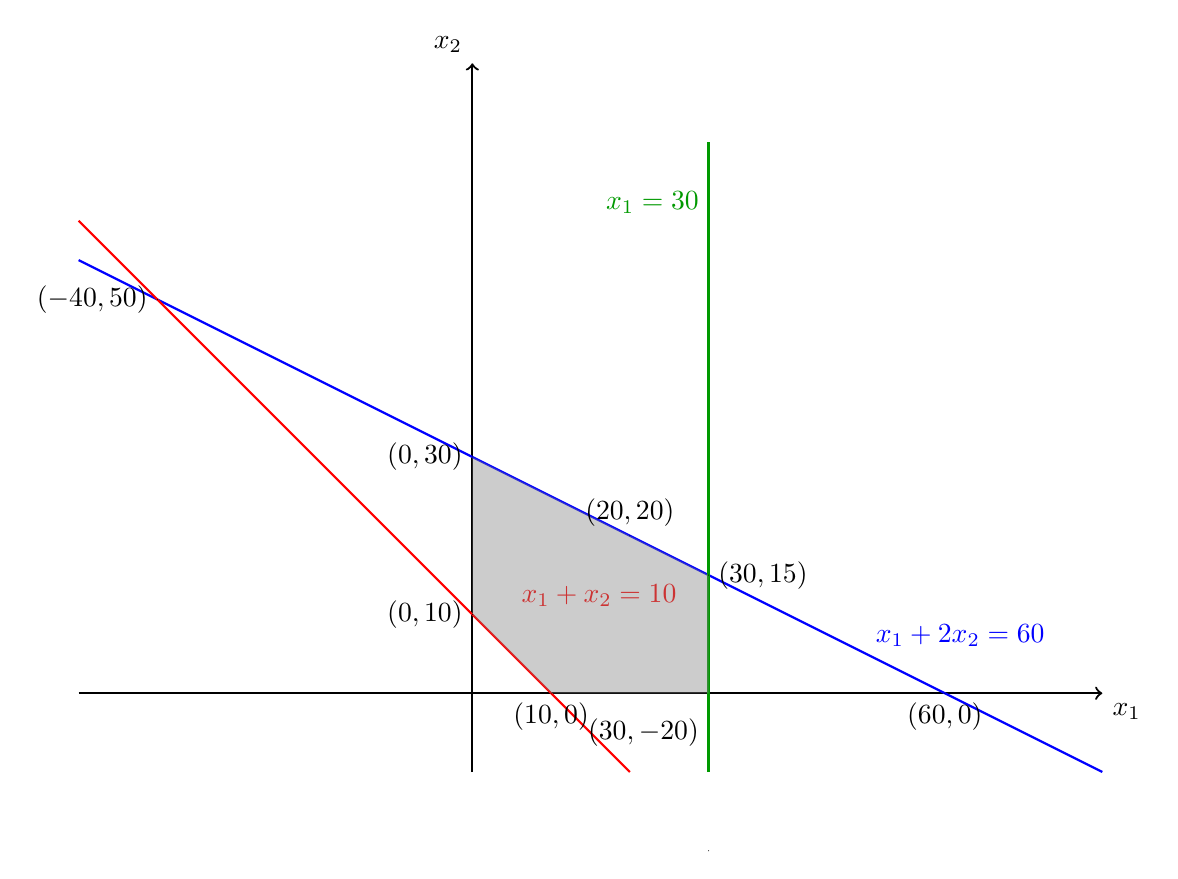
\begin{tikzpicture}[scale=0.1]

% Ejes coordenados
\draw[thick,->] (-50,0) -- (80,0) node[anchor=north west] {$x_1$};
\draw[thick,->] (0,-10) -- (0,80) node[anchor=south east] {$x_2$};

% Restricción 1: x1 + 2x2 <= 60
\draw[thick,blue] (-50,55) -- (80,-10);
\node[blue,anchor=north west] at (50,10) {$x_1 + 2x_2 = 60$};

% Restricción 2: x1 + x2 >= 10
\draw[thick,red] (-50,60) -- (20,-10);
\node[red,anchor=north west] at (5,15) {$x_1 + x_2 = 10$};

% Restricción 3: x1 <= 30
\draw[thick,green!60!black] (30,-10) -- (30,70);
\node[green!60!black,anchor=north east] at (30,65) {$x_1 = 30$};

% Región factible
\fill[gray,opacity=0.4] (10,0) -- (0, 10) -- (0,30) -- (30,15) -- (30,0);

% Intersecciones dentro y fuera de la región factible
% Intersección 1: x1 + 2x2 = 60 y x1 + x2 = 10
\fill[black] (20,20) circle (2pt);
\node[anchor=south] at (20,20) {$(20,20)$};

% Intersección 2: x1 + 2x2 = 60 y x1 = 30
\fill[black] (30,15) circle (2pt);
\node[anchor=west] at (30,15) {$(30,15)$};

% Intersección 3: x1 + x2 = 10 y x1 = 30
\fill[black] (30,-20) circle (2pt);
\node[anchor=east] at (30,-5) {$(30,-20)$};

% Intersección 4: x1 + 2x2 = 60 y eje x2
\fill[black] (60,0) circle (2pt);
\node[anchor=north] at (60,0) {$(60,0)$};

% Intersección 5: x1 + x2 = 10 y eje x2
\fill[black] (10,0) circle (2pt);
\node[anchor=north] at (10,0) {$(10,0)$};

% Intersección 6: x1 + x2 = 10 y eje x1
\fill[black] (0,10) circle (2pt);
\node[anchor=east] at (0,10) {$(0,10)$};

% Intersección 7: x1 + 2x2 = 60 y eje x1
\fill[black] (0,30) circle (2pt);
\node[anchor=east] at (0,30) {$(0,30)$};

% Intersección 8: x1 + 2x2 = 60 y eje x1
\fill[black] (-40,50) circle (2pt);
\node[anchor=east] at (-40,50) {$(-40,50)$};

\end{tikzpicture}
\end{center}


\begin{enumerate}
    \item \textbf{Tipo 1: solución no básica y factible.}
    La solución donde $x_1 = 10$ y $x_2=1$ es no básica y factible porque:
    \begin{itemize}
        \item $h_1>0$, la solución no está sobre la restricción 1 y cumple dicha restricción.
        \item $h_2>0$, la solución no está sobre la restricción 1 y cumple dicha restricción.
        \item $h_3>0$, la solución no está sobre la restricción 3 y cumple dicha restricción.
    \end{itemize}
    La solución tiene cinco componentes no nulas (más que restricciones) así que es no básica y no se incumple ninguna restricción y satisface las restricciones de no negatividad, así que es factible.
    \item \textbf{Tipo 2: solución básica y factible.}
    La solución donde $x_1 = 10$ y $x_2=0$ es básica y factible porque:
    \begin{itemize}
        \item $h_1>0$, la solución no está sobre la restricción 1 y cumple dicha restricción.
        \item $h_2=0$, la solución está sobre la restricción 2.
        \item $h_3>0$, la solución no está sobre la restricción 3 y cumple dicha restricción.
    \end{itemize}
    
    La solución tiene tres componentes no nulas, es básica, no se incumple ninguna restricción y satisface las restricciones de no negatividad, es factible.
    \item \textbf{Tipo 3: solución básica y no factible.}
        La solución donde $x_1 = -40 < 0$ y $x_2=50$ es básica y no factible porque:
    \begin{itemize}
        \item $h_1=0$, la solución está sobre la restricción 1.
        \item $h_2=0$, la solución está sobre la restricción 2.
        \item $h_3>0$, la solución no está sobre la restricción 3 y cumple dicha restricción.
    \end{itemize}
    La solución tiene tres componentes no nulas, es básica, y se incumplen  las restricciones de no negatividad, es no factible.

    \textcolor{red}{\textbf{Error frecuente} \\
    Elegir tres variables y asignarles valor diferente de cero -alguno negativo- y el asignar al resto de variables valor nulo.\\
    Si se eligen tres variables como no nulas y el resto nulas, las tres primeras deben corresponder a una base y, por lo tanto, deben tener los valores resultantes de resolver las ecuaciones cuando se eliminan las variables no básicas.\\
    Por ejemplo, una solución del tipo $x^T=\begin{array}{ccccc}(-100 & -100 & -5 & 0 & 0)\end{array}$ no es básica porque cuando se seleccionan como variables básicas $x_1$, $x_2$ y $h_1$, es decir, si $h_2=h_3=0$, los valores de $x_1$, $x_2$ y $h_1$ no son, respectivamente -100, -100 y -5.}
    
    \item \textbf{Tipo 4: solución no básica y no factible.}
    La solución donde $x_1 = -1 < 0$ y $x_2=-1$ es básica y no factible porque:
    \begin{itemize}
        \item $h_1>0$, la solución no está sobre la restricción 1 y cumple dicha restricción.
        \item $h_2<0$, la solución no está sobre la restricción 3 y no cumple dicha restricción.
        \item $h_3>0$, la solución no está sobre la restricción 3 y cumple dicha restricción.
    \end{itemize}
    La solución tiene más de tres componentes no nulas, es no básica, y se incumple una restricción además de las restricciones de no negatividad, es no factible.
    \item \textbf{¿Cuál de los cuatro tipos de soluciones anteriores cumple que sus soluciones siempre ofrecen mejores valores de la función objetivo que las de cualesquiera otro de los tipos?}
    
    No se puede afirmar nada, porque no hay garantías de que toda las soluciones de un tipo tengan mejor función objetivo que los de las soluciones de otro tipo.

    \textcolor{red}{\textbf{Error frecuente} \\
    Ofrecer un conjunto de valores que no cumplen con las ecuaciones\\
    Indicar que la soluciones de tipo 2 son más interesantes que las restantes. En este apartado se preguntaba por el tipo de solución es siempre mejor que el resto y esto no ocurre para ninguna de ellas. Podemeos encontrar soluciones factibles y no básicas y con mejor función objetivo que otras básicas y factibles.\\    
    No se trata de enunciar lo que dice el teorema fundamental sino de responder a la pregunta específica que se hacía tal y como se indica.}

    \item \textbf{Un valor que sea cota inferior del problema dual de (P)}.
    
    El valor de la función objetivo de cualquier solución factible de (P) es cota inferior de su dual; por ejemplo 60 (valor de la función objetivo de la solución factible $x_1=0$, $x_2=30$).

\end{enumerate}
\clearpage
\section{toyco a}
\input{ejercicios/toyco_a}
\subsection*{Solución}
TOYCO produce y vende tres tipos de juguetes: trenes, camiones y coches. 
Cada juguete requiere un proceso de ensamblaje y uno final de empaquetado. 

Los límites semanales  en los tiempos disponibles para las dos operaciones son \textbf{4300 y 4600}, respectivamente, y los márgenes por tren, camión y coche son de \textbf{2, 3 y 5 }euros, respectivamente. Los tiempos de montaje

Los tiempos que requiere cada tren un cada proceso son \textbf{2, 3} minutos, respectivamente. Los de cada camión son \textbf{2 y 4} y los de cada coche \textbf{4 y 4} minutos.

Adémas, existe un compromiso comercial con un distribuidor de juguetes de suministrarle al menos \textbf{1000} unidades entre camiones y coches.

Si $x_1$, $x_2$ y $x_3$ representan el número semanal de unidades producidas de trenes, camiones y coches, respectivamente, el modelo de programación lineal que permite establecer la producción con mayor margen es el siguiente.


\begin{equation}
\begin{split}
\mbox{max. } z = 2x_1 + 3x_2 + 5x_3\\
s.a.:\\
2x_1 + 2x_2 + 4x_3 \leq 4300\\
3x_1 + 4x_2 + 4x_3 \leq 4600\\
        x_2 +  x_3 \geq 1000\\
x_1,\,\,x_2,\,\,x_3\geq 0\\
\end{split}
\end{equation}

La tabla del método del simplex correspondiente a la solución óptima es:

\begin{center}
\begin{tabular}{c|c|cccccc|}
 & $z$ & $x_1$ & $x_2$ & $x_3$ & $h_1$ & $h_2$ & $h_3$\\ 
      & -5450 & $-3/4$ & 0 & 0 & -1 & $-1/4$ & 0 \\ 
\hline
$x_3$ & 1000  & $1/4$ & 0 & 1 & $1/2$ & $-1/4$ & 0\\ 
$h_3$ & 150  & $3/4$ & 0 & 0 & 0 & $1/4$ & 1\\ 
$x_2$ & 150  & $1/2$ & 1 & 0 & $-1/2$ & $1/2$ & 0\\ 
\hline
\end{tabular}
\end{center}





Se pide:

\begin{enumerate}
    \item Interpretar la información que ofrece a Toyco la tabla de la solución óptima.

    De acuerdo con los valores de las variables en la solución óptima:
    \begin{itemize}
        \item No se produce ningún tren.
        \item Se producen 150 camiones.
        \item Se producen 1000 coches.
        \item Se hace uso de todos los minutos de montaje.
        \item Se hace uso de todos los minutos de empaquetado.
        \item Se sirven 150 unidades por encima del mínimo del compromiso comercial adquirido.
        \item El margen total semanal es de 5450 euros.
    \end{itemize}

    \item Dentro de qué rango de valores del tiempo disponible de empaquetado la gama de productos del plan óptima de producción no cambiaría.

    \begin{equation}
    \begin{split}
    u^B=B^{-1}b = \begin{pmatrix}
    \frac{1}{2} & \frac{-1}{4} & 0\\
    0 & \frac{1}{4} & -1\\
    \frac{-1}{2} & \frac{1}{2} & 0\\
    \end{pmatrix}
    \begin{pmatrix}
    4300\\
    b_2\\
    1000\\
    \end{pmatrix}
     = \begin{pmatrix}
    2150 - \frac{b_2}{4}\\
    \frac{b_2}{4} - 1000\\
    -2150 + \frac{b_2}{2}\\
    \end{pmatrix}
    \geq 0 \Rightarrow \\
    4300 \leq b_2 \leq 8600
    \end{split}
    \end{equation}

    Siempre y cuando se disponga de una cantidad de minutos de montaje igual o superior a 4300 y menor o igual que 8500 la gama de productos sería la misma.

    \item ¿Cuál sería el impacto de relajar el compromiso comercial adquirido?

    El precio sombra de la tercera restricción es 0 ($\pi_3=V^B_{h_3}$, por ser restricción de tipo mayor o igual), con lo que aumentar o reducir entorno al compromiso actual de entregar 100 unidades no cambiaría el plan de producción. De hecho, Toyco está entregando 150 unidades por encima de la cantidad acordada.

    \item Por política de empresa, hay que fabricar al menos tantos trenes como camiones, ¿como afectaría esto al plan óptimo de producción?

    Este nuevo requisito daría lugar a una nueva restricción: $x_1 \geq x_2$, equivalente a $x_1 - x_2 \geq 0$ o, como restricción de igualdad, $x_1 - x_2 - h_4 = 0$.


    \begin{center}
    \begin{tabular}{c|c|ccccccc|}
      & $z$ & $x_1$ & $x_2$ & $x_3$ & $h_1$ & $h_2$ & $h_3$ & $h_3$\\ 
      & -5450 & -3/4 & 0 & 0 & -1 & -1/4 & 0 & 0\\ 
    \hline
    $x_3$ & 1000  & $\frac{1}{4}$ & 0 & 1 & $\frac{1}{2}$ & $\frac{-1}{4}$ & 0 & 0 \\ 
    $h_3$ & 150  & $\frac{3}{4}$ & 0 & 0 & 0 & $\frac{1}{4}$ & 1 & 0\\ 
    $x_2$ & 150  & $\frac{1}{2}$ & 1 & 0 & $\frac{-1}{2}$ & $\frac{1}{2}$ & 0 & 0\\ 
    \hline
          & 0     & 1          & -1  & 0 & 0 & 0 & 0 & -1\\           
    \hline
    $h_4$ & -150   & $-\frac{3}{2}$ & 0  & 0 & $\frac{1}{2}$ & $-\frac{1}{2}$ & 0 & 1\\ 
    \hline
       & -5375 & 0 & 0 & 0 & $\frac{-5}{4}$ & 0 & 0 & $\frac{-1}{2}$ \\ 
    \hline
    $x_3$ & 975  & 0 & 0 & 1 & $\frac{7}{12}$ & $\frac{-1}{3}$ & 0 & $\frac{1}{6}$\\ 
    $h_3$ & 75  & 0 & 0 & 0 & $\frac{1}{4}$ & 0 & 1 & $\frac{1}{2}$\\ 
    $x_2$ & 100  & 0 & 1 & 0 & $\frac{-1}{3}$ & $\frac{1}{3}$ & 0 & $\frac{1}{3}$\\ 
    $x_1$ & 100  & 1 & 0 & 0 & $\frac{-1}{3}$ & $\frac{1}{3}$ & 0 & $\frac{-2}{3}$\\ 
    \hline
      & -5375 & 0 & 0 & 0 & $\frac{-5}{4}$ & 0 & 0 & $\frac{-1}{2}$ \\ 
    \hline
    $x_3$ & 1075  & 1 & 0 & 1 & $\frac{1}{4}$ & 0 & 0 & $\frac{-1}{2}$\\ 
    $h_3$ & 75  & 0 & 0 & 0 & $\frac{1}{4}$ & 0 & 1 & $\frac{1}{2}$\\ 
    $x_2$ & 0  & -1 & 1 & 0 & 0 & 0 & 0 & 1\\ 
    $h_2$ & 300  & 3 & 0 & 0 & -1 & 1 & 0 & -2\\ 
    \hline
    \end{tabular}
    \end{center}

    La solución óptima no cumple con la nueva restricción, lo cual hace que la solución básica correspondiente no sea factible ($h_4 = -150 \leq 0$). Aplicando Lemke se puede llegar a dos posibles soluciones alternativas. En ambas el margen total es de 5375 euros. Además:
    \begin{itemize}
        \item En una de ellas se fabrican 100 trenes, 100 camiones y 975 coches.
        \item En la otra solución se fabrican únicamente 1075 coches (no se fabrican trenes ni coches, con lo que el requisito comercial se cumple).
    \end{itemize}



    
\end{enumerate}

\clearpage
\section{toyco b}
Toyco produce y vende tres tipos de juguetes: trenes, camiones y coches. 
Cada juguete requiere un proceso de ensamblaje y uno final de empaquetado. 

Los límites semanales  en los tiempos disponibles para las dos operaciones son \textbf{4300 y 4600}, respectivamente, y los márgenes por tren, camión y coche son de \textbf{1, 2 y 5 }euros, respectivamente. 

Los tiempos que requiere cada tren un cada proceso (ensamble y empaquetado) son \textbf{2, 1} minutos, respectivamente. Los de cada camión son \textbf{2 y 2} y los de cada coche \textbf{1 y 4} minutos.

Además, existe un compromiso comercial con un distribuidor de juguetes de suministrarle al menos \textbf{1000} unidades entre camiones y coches.

Si $x_1$, $x_2$ y $x_3$ representan el número semanal de unidades producidas de trenes, camiones y coches, respectivamente, el modelo de programación lineal que permite establecer la producción con mayor margen es el siguiente.

\begin{equation}
\begin{split}
\mbox{max. } z =  x_1 + 2x_2 + 5x_3\\
s.a.:\\
2x_1 + 2x_2 +  x_3 \leq 4300\\
 x_1 + 2x_2 + 4x_3 \leq 4600\\
        x_2 +  x_3 \geq 1000\\
x_1,\,\,x_2,\,\,x_3\geq 0\\
\end{split}
\end{equation}

\begin{center}
\begin{tabular}{c|c|cccccc|}
 & $z$ & $x_1$ & $x_2$ & $x_3$ & $h_1$ & $h_2$ & $h_3$\\ 
Phase 2 & -5750 & $-1/4$ & $-1/2$ & 0 & 0 & $-5/4$ & 0 \\ 
\hline
$h_1$ & 3150  & $7/4$ & $3/2$ & 0 & 1 & $-1/4$ & 0\\ 
$h_3$ & 150  & $1/4$ & $-1/2$ & 0 & 0 & $1/4$ & 1\\ 
$x_3$ & 1150  & $1/4$ & $1/2$ & 1 & 0 & $1/4$ & 0\\ 
\hline
\end{tabular}
\end{center}





Se pide:

\begin{enumerate}
    \item Interpretar la información que ofrece la tabla de la solución óptima (producción, margen total y recusos y compromiso comercial).
    
    \item Calcular dentro de qué rango de valores del tiempo disponible de empaquetado la gama de productos del plan óptima de producción no cambiaría.
    
    \item Explicar cuál sería el impacto de relajar el compromiso comercial adquirido

    \item Indicar y justificar cómo afectaría esto al plan óptimo de producción si, por política de empresa, hubiera que que fabricar al menos tantos camiones como coches.
   
\end{enumerate}








\subsection*{Solución}
TOYCO produce y vende tres tipos de juguetes: trenes, camiones y coches. 
Cada juguete requiere un proceso de ensamblaje y uno final de empaquetado. 

Los límites semanales  en los tiempos disponibles para las dos operaciones son \textbf{4300 y 4600}, respectivamente, y los márgenes por tren, camión y coche son de \textbf{1, 2 y 5 }euros, respectivamente. Los tiempos de montaje

Los tiempos que requiere cada tren un cada proceso son \textbf{2, 1} minutos, respectivamente. Los de cada camión son \textbf{2 y 2} y los de cada coche \textbf{1 y 4} minutos.

Además, existe un compromiso comercial con un distribuidor de juguetes de suministrarle al menos \textbf{1000} unidades entre camiones y coches.

Si $x_1$, $x_2$ y $x_3$ representan el número semanal de unidades producidas de trenes, camiones y coches, respectivamente, el modelo de programación lineal que permite establecer la producción con mayor margen es el siguiente.

\begin{equation}
\begin{split}
\mbox{max. } z =  x_1 + 2x_2 + 5x_3\\
s.a.:\\
2x_1 + 2x_2 +  x_3 \leq 4300\\
 x_1 + 2x_2 + 4x_3 \leq 4600\\
        x_2 +  x_3 \geq 1000\\
x_1,\,\,x_2,\,\,x_3\geq 0\\
\end{split}
\end{equation}

\begin{center}
\begin{tabular}{c|c|cccccc|}
 & $z$ & $x_1$ & $x_2$ & $x_3$ & $h_1$ & $h_2$ & $h_3$\\ 
Fase 2 & -5750 & $-1/4$ & $-1/2$ & 0 & 0 & $-5/4$ & 0 \\ 
\hline
$h_1$ & 3150  & $7/4$ & $3/2$ & 0 & 1 & $-1/4$ & 0\\ 
$h_3$ & 150  & $1/4$ & $-1/2$ & 0 & 0 & $1/4$ & 1\\ 
$x_3$ & 1150  & $1/4$ & $1/2$ & 1 & 0 & $1/4$ & 0\\ 
\hline
\end{tabular}
\end{center}





Se pide:

\begin{enumerate}
    \item Interpretar la información que ofrece a Toyco la tabla de la solución óptima.

    De acuerdo con los valores de las variables en la solución óptima:
    \begin{itemize}
        \item No se produce ningún tren.
        \item No se produce ningún camión.
        \item Se producen 1150 coches.
        \item No se hace uso de 3150 minutos de los 4300 disponibles para el montaje.
        \item Se hacen uso de todos los minutos de empaquetado.
        \item Se sirven 150 unidades por encima del mínimo del compromiso comercial adquirido.
        \item el margen total semanal es de 5750 euros.
    \end{itemize}
    

    \item Dentro de qué rango de valores del tiempo disponible de empaquetado la gama de productos del plan óptima de producción no cambiaría.

    \begin{equation}
    \begin{split}
    u^B=B^{-1}b =
    \begin{pmatrix}
    1 & -1/4 & 0\\
    0 & 1/4 & -1\\
    0 & 1/4 & 0\\
    \end{pmatrix}
    \begin{pmatrix}
    4300\\
    b_2\\
    1000\\
    \end{pmatrix}
     = \begin{pmatrix}
    4300 - \frac{b_2}{4}\\
    \frac{b_2}{4} - 1000\\
    \frac{b_2}{4}\\
    \end{pmatrix}
    \geq 0 \Rightarrow \\
    4000 \leq b_2 \leq 17200
    \end{split}
    \end{equation}

    Siempre y cuando se disponga de una cantidad de minutos de montaje igual o superior a 4000 y menor o igual que 17200 la gama de productos sería la misma.

    \item ¿Cuál sería el impacto de relajar el compromiso comercial adquirido?

    El precio sombra de la tercera restricción es 0 ($\pi_3=V^B_{h_3}$, por ser restricción de tipo mayor o igual), con lo que aumentar o reducir entorno al compromiso actual de entregar 1000 unidades no cambiaría el plan de producción. De hecho, Toyco está entregando 150 unidades por encima de la cantidad acordada.

    \item Por política de empresa, hay que fabricar al menos tantos camiones como coches, ¿como afectaría esto al plan óptimo de producción?

    Este nuevo requisito daría lugar a una nueva restricción: $x_2 \geq x_3$, equivalente a $x_2 - x_3 \geq 0$ o, como restricción de igualdad, $x_2 - x_3 - h_4 = 0$.

    \begin{center}
    \begin{tabular}{c|c|ccccccc|}
     & $z$ & $x_1$ & $x_2$ & $x_3$ & $h_1$ & $h_2$ & $h_3$ & $h_4$\\ 
           & -5750 & $-1/4$ & $-1/2$ & 0 & 0 & $-5/4$ & 0 & 0\\ 
    \hline
    $h_1$ & 3150  & $7/4$ & $3/2$ & 0 & 1 & $-1/4$ & 0 & 0\\ 
    $h_3$ & 150  & $1/4$ & $-1/2$ & 0 & 0 & $1/4$ & 1 & 0\\ 
    $x_3$ & 1150  & $1/4$ & $1/2$ & 1 & 0 & $1/4$ & 0 & 0\\ 
    \hline
          & 0     & 0     & 1     &   -1 & 0 & 0 & 0 & -1\\           
    \hline
    $h_4$ & -1150  & -1/4 & -3/2  & 0 & 0 & -1/4  & 0 & 1\\ 
    \hline
          & -5750 & $-1/4$ & $-1/2$ & 0 & 0 & $-5/4$ & 0 & 0\\ 
    \hline
    $h_1$ & 3150  & $7/4$ & $3/2$ & 0 & 1 & $-1/4$ & 0 & 0\\ 
    $h_3$ & 150  & $1/4$ & $-1/2$ & 0 & 0 & $1/4$ & 1 & 0\\ 
    $x_3$ & 1150  & $1/4$ & $1/2$ & 1 & 0 & $1/4$ & 0 & 0\\ 
    $h_4$ & -1150  & -1/4 & -3/2  & 0 & 0 & -1/4  & 0 & 1\\ 
    \hline
          & $-16100/3$ & $-1/6$ & 0 & 0 & 0 & $-7/6$ & 0 & $-1/3$ \\ 
    \hline
    $h_1$ & 2000  & $3/2$ & 0 & 0 & 1 & $-1/2$ & 0 & 1\\ 
    $h_3$ & 1600/3  & $1/3$ & 0 & 0 & 0 & $1/3$ & 1 & $-1/3$\\ 
    $x_3$ & 2300/3  & $1/6$ & 0 & 1 & 0 & $1/6$ & 0 & $1/3$\\ 
    $x_2$ & 2300/3  & $1/6$ & 1 & 0 & 0 & $1/6$ & 0 & $-2/3$\\ 
    \hline
    \end{tabular}
    \end{center}

    La solución óptima no cumple con la nueva restricción, lo cual hace que la solución básica correspondiente no sea factible ($h_4 = -1150 \leq 0$). Aplicando Lemke se llega a la solución óptima, con un beneficio de 16100/3 euros. Además, se fabrican 2300/3 camiones, 2300/3 coches y no se fabrican trenes.
   
\end{enumerate}








\clearpage
\section{transporte5 eulerhamilton}


El grafo asociado a un problema de transporte con cinco plantas (orígenes) y cinco almacenes (destinos) es un grafo dirigido. Si el mismo grafo fuera no dirigido:
\begin{itemize}
    \item Indica un ciclo euleriano en dicho grafo no dirigido.
    \item Indica un ciclo hamiltoniano en dicho grafo no dirigido.
    \item ¿Existen ciclos euleriano para cualquier número de orígenes y destinos?
    \item ¿Existen ciclos hamiltonianos para cualquier número de orígenes y destinos?

\end{itemize}
\subsection*{Solución}
El grafo asociado a un problema de transporte con cinco plantas (orígenes) y cinco almacenes (destinos) es un grafo dirigido. Si el mismo grafo fuera no dirigido:
\begin{itemize}
    \item Indica un ciclo euleriano en dicho grafo no dirigido. \textit{Un grafo conexo no dirigido contiene un ciclo euleriano si y solo si todos sus vértices tienen grado par. En el grafo no dirigido todos los nodos tienen grado 5; luego   no contiene un ciclo euleriano.}
    \item Indica un ciclo hamiltoniano en dicho grafo no dirigido.  \textit{Existen  muchos ciclos hamiltonianos. Si se llaman $O_i$ los nodos origen y $D_j$ los nodos destino, un posible ciclo hamiltoniano sería: $O_1 \rightarrow D_1 \rightarrow O_2 \rightarrow D_2 \rightarrow O_3 \rightarrow D_3 \rightarrow O_4 \rightarrow D_4 \rightarrow O_5 \rightarrow D_5 \rightarrow O_1$}
    \item ¿Existen ciclos euleriano para cualquier número de orígenes y destinos? \textit{Si el número de orígenes y de destinos es par, existirán ciclos eulerianos.} 
    \item ¿Existen ciclos hamiltonianos para cualquier número de orígenes y destinos? \textit{Si el número de orígenes y destinos es el mismo, existirán ciclos hamiltoniano  (y al menos hay dos orígenes y dos destinos).}


\end{itemize}


\clearpage
\section{transporte tasassutitucion}
La siguiente tabla indica el valor de las variables de un problema de transporte con las ofertas de los orígenes $O_i$ y las demandas de los destinos $D_j$. Indica cuáles son los vectores de tasas de sustitución de las variables $x_{14}$ y $x_{22}$.

Nota: la celda correspondiente a la fila $i$ y a la columna $j$ contiene el valor de la variable $x_{ij}$, e indica la cantidad de producto que se transporta desde el origen $i$ al destino $j$.

\begin{table}[h]
\begin{center}

\begin{tabular}{ccccccc}
                      &                         &                        &                        &                        &                         & $O_i$ \\ \cline{2-6}
\multicolumn{1}{l|}{} & \multicolumn{1}{l|}{10} & \multicolumn{1}{l|}{}  & \multicolumn{1}{l|}{}  & \multicolumn{1}{l|}{}  & \multicolumn{1}{l|}{}   & 10    \\ \cline{2-6}
\multicolumn{1}{l|}{} & \multicolumn{1}{l|}{5}  & \multicolumn{1}{l|}{5} & \multicolumn{1}{l|}{5} & \multicolumn{1}{l|}{}  & \multicolumn{1}{l|}{}   & 15    \\ \cline{2-6}
\multicolumn{1}{l|}{} & \multicolumn{1}{l|}{}   & \multicolumn{1}{l|}{}  & \multicolumn{1}{l|}{5} & \multicolumn{1}{l|}{5} & \multicolumn{1}{l|}{10} & 20    \\ \cline{2-6}
$D_j$                 & 15                      & 5                      & 10                     & 5                      & 10                      &      
\end{tabular}
    
\end{center}
\end{table}
\subsection*{Solución}
La siguiente tabla indica el valor de las variables de un problema de transporte con las ofertas de los orígenes $O_i$ y las demandas de los destinos $D_j$. \textbf{Indica cuáles son los vectores de tasas de sustitución de las variables $x_{14}$ y $x_{22}$}.

Nota: la variable $x_{ij}$ (fila $i$, columna $j$) indica la cantidad de producto que se mueve desde el origen $i$ al destino $j$.

\begin{table}[h]
\begin{center}

\begin{tabular}{ccccccc}
                      &                         &                        &                        &                        &                         & $O_i$ \\ \cline{2-6}
\multicolumn{1}{l|}{} & \multicolumn{1}{l|}{10} & \multicolumn{1}{l|}{}  & \multicolumn{1}{l|}{}  & \multicolumn{1}{l|}{}  & \multicolumn{1}{l|}{}   & 10    \\ \cline{2-6}
\multicolumn{1}{l|}{} & \multicolumn{1}{l|}{5}  & \multicolumn{1}{l|}{5} & \multicolumn{1}{l|}{5} & \multicolumn{1}{l|}{}  & \multicolumn{1}{l|}{}   & 15    \\ \cline{2-6}
\multicolumn{1}{l|}{} & \multicolumn{1}{l|}{}   & \multicolumn{1}{l|}{}  & \multicolumn{1}{l|}{5} & \multicolumn{1}{l|}{5} & \multicolumn{1}{l|}{10} & 20    \\ \cline{2-6}
$D_j$                 & 15                      & 5                      & 10                     & 5                      & 10                      &      
\end{tabular}
    
\end{center}
\end{table}

\textbf{Solución}
\vspace{0.5cm}

\begin{tabular}{|l|c|c|}
\hline
 & $x_{14}$ & $x_{22}$ \\
\hline
$x_{11}$ & 1 & 0 \\
$x_{21}$ & -1 & 0 \\
$x_{22}$ & 0 & 1 \\
$x_{23}$ & 1 & 0 \\
$x_{33}$ & -1 & 0 \\
$x_{34}$ & 1 & 0 \\
$x_{35}$ & 0 & 0 \\
\hline
\end{tabular}


\clearpage
\section{transporte vogel degenerada}
Una empresa fabrica el mismo modelo de coche en cuatro fábricas diferentes. Una vez fabricados los coches se transportan a una campa que existe en cada uno de lo los cinco continentes en los que la empresa vende su vehículo.

Las capacidades (en cientos de miles de coches) de cada fábrica son 10, 20, 15 y 20. Las demandas de cada continente son respectivamente 15, 10, 15, 15 y 10.

La siguiente tabla indica los costes de transporte de un coche desde una fábrica (fila) a un continente (columna).

\begin{table}[h]
\begin{center}
\begin{tabular}{|c|c|c|c|c|}
\hline
4 & 2 & 3 & 5 & 1 \\ \hline
5 & 2 & 7 & 3 & 8 \\ \hline
6 & 4 & 4 & 3 & 7 \\ \hline
1 & 2 & 5 & 3 & 4 \\ \hline
\end{tabular}
\end{center}
\end{table}

\begin{enumerate}
    \item \textbf{Aplica} el método de Vogel para encontrar una solución inicial de este problema de transporte.
    \item ¿Qué \textbf{características} tiene la solución que se ha obtenido aplicando el método de Vogel?¿Por qué?
\end{enumerate}





\subsection*{Solución}
Una empresa fabrica el mismo modelo de coche en cuatro fábricas diferentes. Una vez fabricados los coches se transportan a una campa que existe en cada uno de lo los cinco continentes en los que la empresa vende su vehículo.

Las capacidades (en cientos de miles de coches) de cada fábrica son 10, 20, 15 y 20. Las demandas de cada continente son respectivamente 15, 10, 15, 15 y 10.

La siguiente tabla indica los costes de transporte de un coche desde una fábrica (fila) a un continente (columna).

\begin{table}[h]
\begin{center}
\begin{tabular}{|c|c|c|c|c|}
\hline
4 & 2 & 3 & 5 & 1 \\ \hline
5 & 2 & 7 & 3 & 8 \\ \hline
6 & 4 & 4 & 3 & 7 \\ \hline
1 & 2 & 5 & 3 & 4 \\ \hline
\end{tabular}
\end{center}
\end{table}

\begin{enumerate}
    \item \textbf{Aplica} el método de Vogel para encontrar una solución inicial de este problema de transporte.
   
    
    \item ¿Qué \textbf{características} tiene la solución que se ha obtenido aplicando el método de Vogel?¿Por qué?

     
    El problema está equilibrado.

    Una posible solución al aplicar el método de Vogel es ésta (hay más posibles dados los empates que aparecen):

\begin{table}[h!]
\begin{center}
\begin{tabular}{|l|l|l|l|l|}
\hline
   &    &    &    & 10 \\ \hline
   & 10 &    & 10 &    \\ \hline
   &    & 15 &    &    \\ \hline
15 &    &    & 5  &    \\ \hline
\end{tabular}
\end{center}
\end{table}
    Esta solución es:
    \begin{itemize}
        \item básica, el número de variables no nulas es menor de 4+5-1=8.
        \item factible, cumple las 9 restricciones.
        \item degenerada, sólo tiene 6 variables básicas no nulas.
        \item óptima, no existen costes reducidos positivos.
    \end{itemize}
\end{enumerate}


\clearpage
\section{voluntarios unidos}
La organización \textbf{Voluntarios Unidos} coordina actividades de apoyo comunitario en tres áreas: \textbf{educación (E)}, \textbf{salud (S)} y \textbf{medio ambiente (M)}. Los voluntarios tienen un tiempo limitado semanal y la organización desea maximizar el impacto de sus actividades, medido en términos de puntos de beneficio para la comunidad.

Por cada hora dedicada, cada área genera los siguientes beneficios. Educación: \textbf{5 puntos} de beneficio, salud: \textbf{8 puntos} de beneficio y medio ambiente: \textbf{6 puntos} de beneficio.

La organización cuenta con un máximo de \textbf{40 horas de trabajo voluntario semanalmente}. 

Además, por política interna, al menos el \textbf{30\% del tiempo total} debe destinarse a actividades educativas.

Por último, la organización desea un beneficio de al menos 200 puntos entre las actividades de educación y salud.

Si $x_1$, $x_2$, $x_3$ representan el tiempo semanal dedicado (en horas) a educación, salud y medio ambiente, respectivamente, el modelo de programación lineal que permite maximizar el impacto comunitario es:


\begin{equation}
\begin{split}
\text{max. } z \quad = 5x_1 + 8x_2 + 6x_3 \\
\text{s.a.:} \\
\quad x_1 + x_2 + x_3 \leq 40 \quad \text{(Tiempo total disponible)} \\
\quad 0.7x_1 - 0.3x_2 - 0.3x_3 \geq 0 \quad \text{(Política educativa)}\\
\quad 5x_1 + 8x_2 \geq 200 \quad \text{(Límite en salud y medio ambiente)} \\
\end{split}
\end{equation}


Que se puede formular de manera equivalente de la siguiente manera:


\begin{equation}
\begin{split}
\text{max. } z = 5x_1 + 8x_2 + 6x_3 \\
\text{s.a.:} \\
x_1 + x_2 + x_3 \leq 40 \quad \text{(Tiempo total disponible)} \\
7x_1 - 3x_2 - 3x_3 \geq 0 \quad \text{(Política educativa)} \\
5x_1 + 8x_2 \geq 200 \quad \text{(Límite en salud y medio ambiente)} \\
x_1, x_2, x_3 \geq 0 \quad \text{(No negatividad)}
\end{split}
\end{equation}

Se conoce la tabla correspondiente a la solución óptima del problema:

\begin{center}
\begin{tabular}{c|c|cccccc|}
 & $z$ & $x_1$ & $x_2$ & $x_3$ & $h_1$ & $h_2$ & $h_3$\\ 
      & -284 & 0 & 0 & -2 & $-71/10$ & $-3/10$ & 0 \\ 
\hline
$h_3$ & 84  & 0 & 0 & 8 & $71/10$ & $3/10$ & 1\\ 
$x_1$ & 12  & 1 & 0 & 0 & $3/10$ & $-1/10$ & 0\\ 
$x_2$ & 28  & 0 & 1 & 1 & $7/10$ & $1/10$ & 0\\ 
\hline
\end{tabular}
\end{center}

Se pide:

\begin{enumerate}
    \item Interpretar la información que ofrece la tabla de la solución óptima en términos de las actividades que se cumplen, los beneficios generados y el cumplimiento de requisitos.

    \item Obtener la inversa de la base correspondiente a la solución óptima.

    \item Evaluar el impacto sobre las horas dedicadas a las diferentes actividades y sobre el beneficio de las actividades realizadas si, en una semana en particular, fuera necesario dedicar una hora a actividades relacionadas con medio ambiente.

    \item Cuantificar el impacto sobre las horas dedicadas a cada actividad y sobre los puntos de beneficio si, como resultado de la celebración de la semana de voluntariado se dispusiera de un número genérico de horas adicionales a las 40 semanales igual a $H$.
    
\end{enumerate}





\subsection*{Solución}
La organización \textbf{Voluntarios Unidos} coordina actividades de apoyo comunitario en tres áreas: \textbf{educación (E)}, \textbf{salud (S)} y \textbf{medio ambiente (M)}. Los voluntarios tienen un tiempo limitado semanal y la organización desea maximizar el impacto de sus actividades, medido en términos de puntos de beneficio para la comunidad.

Por cada hora dedicada, cada área genera los siguientes beneficios. Educación: \textbf{5 puntos} de beneficio, salud: \textbf{8 puntos} de beneficio y medio ambiente: \textbf{6 puntos} de beneficio.

La organización cuenta con un máximo de \textbf{40 horas de trabajo voluntario semanalmente}. 

Además, por política interna, al menos el \textbf{30\% del tiempo total} debe destinarse a actividades educativas.

Por último, la organización desea un beneficio de al menos 200 puntos entre las actividades de educación y salud.

Si $x_1$, $x_2$, $x_3$ representan el tiempo semanal dedicado (en horas) a educación, salud y medio ambiente, respectivamente, el modelo de programación lineal que permite maximizar el impacto comunitario es:


\begin{equation}
\begin{split}
\text{max. } z = 5x_1 + 8x_2 + 6x_3 \\
\text{s.a.:} \\
x_1 + x_2 + x_3 \leq 40 \quad \text{(Tiempo total disponible)} \\
0.7x_1 - 0.3x_2 - 0.3x_3 \geq 0 \quad \text{(Política educativa)}\\
5x_1 + 8x_2 \geq 200 \quad \text{(Límite en salud y medio ambiente)} \\
\end{split}
\end{equation}

Que se puede formular de manera equivalente de la siguiente manera:


\begin{equation}
\begin{split}
\text{max. } z = 5x_1 + 8x_2 + 6x_3 \\
\text{s.a.:} \\
x_1 + x_2 + x_3 \leq 40 \quad \text{(Tiempo total disponible)} \\
7x_1 - 3x_2 - 3x_3 \geq 0 \quad \text{(Política educativa)} \\
5x_1 + 8x_2 \geq 200 \quad \text{(Límite en salud y medio ambiente)} \\
x_1, x_2, x_3 \geq 0 \quad \text{(No negatividad)}
\end{split}
\end{equation}

Se conoce la tabla correspondiente a la solución óptima del problema:
\begin{center}
\begin{tabular}{c|c|cccccc|}
 & $z$ & $x_1$ & $x_2$ & $x_3$ & $h_1$ & $h_2$ & $h_3$\\ 
Phase 2 & -284 & 0 & 0 & -2 & $-71/10$ & $-3/10$ & 0 \\ 
\hline
$h_3$ & 84  & 0 & 0 & 8 & $71/10$ & $3/10$ & 1\\ 
$x_1$ & 12  & 1 & 0 & 0 & $3/10$ & $-1/10$ & 0\\ 
$x_2$ & 28  & 0 & 1 & 1 & $7/10$ & $1/10$ & 0\\ 
\hline
\end{tabular}
\end{center}



Se pide:

\begin{enumerate}
    \item \textbf{Interpretar la información que ofrece la tabla de la solución óptima en términos de las actividades que se cumplen, los beneficios generados y el cumplimiento de requisitos.}

    La programación óptima de actividades consiste en:
    \begin{itemize}
        \item Dedicar 12 horas a educación, 28 horas a salud y ninguna a medio ambiente.
        \item El beneficio total obtenido sería de 284 puntos.
        \item Se haría uso del tiempo total disponible ($h_1=0$).
        \item La proporción de tiempo dedicada a actividades educativas se cumpliría por el mínimo, 30\% ($h_2=0$).
        \item Se cumple con el mínimo de beneficio de las actividades de educación y salud superando el mínimo en 84 puntos ($h_3=84$).
    \end{itemize}

    \item \textbf{Obtener la inversa de la base correspondiente a la solución óptima.}

    Las columna de la inversa de la base de obtienen de la siguiente manera.
    \begin{itemize}
        \item Primera columna: columna de las tasas de sustitución correspondiente a $h_1$ (restricción de tipo menor o igual).
        \item Segunda columna: opuesta de la columna de las tasas de sustitución correspondiente a $h_2$ (restricción de tipo mayor o igual).
        \item Tercera columna: opuesta de la columna de las tasas de sustitución correspondiente a $h_3$ (restricción de tipo mayor o igual).
    \end{itemize}

\begin{equation}
\begin{split}
B^{-1} =\begin{pmatrix}
71/10 & -3/10 & -1\\
3/10 & 1/10 & 0\\
7/10 & -1/10 & 0\\
\end{pmatrix}
\end{split}
\end{equation}
    
    \item \textbf{Evaluar el impacto sobre las horas dedicadas a las diferentes actividades y sobre el beneficio de las actividades realizadas si, en una semana en particular, fuera necesario dedicar una hora a actividades relacionadas con medio ambiente.}

    Este cambio quedaría reflejado en el modelo de programación lineal por el hecho de que $x_3$ tomaría valor 1.  

    \begin{itemize}
        \item El impacto sobre el beneficio se puede calcular a partir del criterio del simplex de $x_3$. Como $V^B_{x_3} = -2$, realizar una hora de actividades de medio ambiente daría lugar a una reducción del beneficio de 2 unidades (sería igual a 282).
        \item El impacto sobre las horas a las actividades se podría evaluar estudiando los cambios de los valores de $x_1$ y $x_2$ y estos cambios vienen dados por las tasas de sustitución correspondientes.
        \begin{itemize}
            \item $p^B_{23} = 0$ representa la disminución del valor de la segunda variable básica ($x_1$) cuando la tercera variable aumenta su valor una unidad ($x_3$=1). Se dedicaría el mismo tiempo a educación, se decir, 12 horas.
            \item $p^B_{33} = 1$ representa la disminución del valor de la tercera variable básica ($x_3$) cuando la tercera variable aumenta su valor una unidad ($x_3$=1). Se dedicaría una hora menos a salud, es decir, 27 horas.
        \end{itemize}
    \end{itemize}

    Por un lado, al dedicar una hora más a medio ambiente, tendríamos 6 puntos de beneficio adicionales y, por otro, al dedicar una hora menos en salud, tendríamos 8 puntos de beneficio menos: el resultado neto es una reducción de 2 unidades del beneficio, como indica $V^B_{x_3}$.


    \item \textbf{Cuantificar el impacto sobre las horas dedicadas a cada actividad y sobre los puntos de beneficio si, como resultado de la celebración de la semana de voluntariado se dispusiera de un número genérico de horas adicionales a las 40 semanales igual a $H$.}

    Si dispusiéramos de $H$ horas adicionales a las 40, cambiaría el término $b$ del problema, que sería:

    \begin{equation}
    b'=
    \begin{pmatrix}
    40 + H \\
    0\\
    200
    \end{pmatrix}    
    \end{equation}

    Al cambiar b, cambiarían los valores de $u^B$ y $z^B$.

    \begin{equation}
    \begin{split}
    u^B=B^{-1}b = \begin{pmatrix}
    71/10 & -3/10 & -1\\
    3/10 & 1/10 & 0\\
    7/10 & -1/10 & 0\\
    \end{pmatrix}
    \begin{pmatrix}
    40 + H\\
    0\\
    200\\
    \end{pmatrix}
     = \begin{pmatrix}
    84+H/10\\
    12+3H/10\\
    28+7H/10
    \end{pmatrix}
    \end{split}
    \end{equation}

    La solución básica correspondiente nunca dejaría de ser factible y se realizarían $3H/10$ horas más de educación y $7H/10$ de salud.

    El impacto sobre los puntos sería el siguiente:

    \begin{equation}
    \begin{split}
    z^B=c^Bu^B = \begin{pmatrix}
    0 & 5 & 8\\
    \end{pmatrix}
    \begin{pmatrix}
    84\\
    12+3H/10\\
    28+7H/10\\
    \end{pmatrix}
     = 284 + 71H/10\end{split}
    \end{equation} 

    Es decir, el beneficio se incrementaria en 71H/10.

    Todo lo anterior se puede observar igualmente, analizando qué ocurriría si hacemos que $h_1 = -H$ que sería análogo a disponer de $H$ horas adicionales de tiempo total disponible.

    Siguiendo un razonamiento análogo al de la pregunta anterior y dado el carácter lineal del problema, se podría realizar el análisis evaluando el impacto de que $\Delta H = -H$, con el mismo resultado.
    

    

    
\end{enumerate}



\clearpage

\end{document}
